\documentclass[12pt]{report}


\usepackage{url}
\usepackage{xspace}
\usepackage{fancybox}
\usepackage{cuthesis}
\usepackage{graphicx}
\usepackage{booktabs}
\usepackage{makecell}
\usepackage{csquotes}
\usepackage{multirow}
\usepackage{pdflscape}
\usepackage{subfigure}
\usepackage{color}
\usepackage[dvipsnames]{xcolor}
\usepackage{adjustbox}
\usepackage{array}
\usepackage{mathtools}
\usepackage[titletoc]{appendix}



\newcolumntype{L}[1]{>{\raggedright\let\newline\\\arraybackslash\hspace{0pt}}m{#1}}
\newcolumntype{C}[1]{>{\centering\let\newline\\\arraybackslash\hspace{0pt}}m{#1}}
\newcolumntype{R}[1]{>{\raggedleft\let\newline\\\arraybackslash\hspace{0pt}}m{#1}}





\linespread{1.6}

\author{Sultan Wehaibi}
\title {The Impact of Self-admitted Technical Debt}
\degree{Master of Applied Science in Software Engineering}
\dept  {Computer Science and Software Engineering}



%%%%%%%%%%%%%%%%%%%%%%%%%%%%%%%%%%%%%%%%%%%%%%%%%%%%%%%%%
% define commands for frequently used words or phrases
%%%%%%%%%%%%%%%%%%%%%%%%%%%%%%%%%%%%%%%%%%%%%%%%%%%%%%%%%
\newcommand{\SATD}{self-admitted technical debt\xspace}
\newcommand{\ie}{i.e.\xspace}
\newcommand{\eg}{e.g.\xspace}
%%%%%%%%%%%%%%%%%%%%%%%%%%%%%%%%%%%%%%%%%%%%%%%%%%%%%%%%%
% define commands for your RQs
%%%%%%%%%%%%%%%%%%%%%%%%%%%%%%%%%%%%%%%%%%%%%%%%%%%%%%%%%
\newcommand{\chapterIIIrqi}{\textbf{RQ1 - Do technical debt files have more bugs? Do files become more buggy after the introduction of technical debt?}}
\newcommand{\chapterIIIrqii}{\textbf{RQ2 - Do technical debt related changes tend to introduce future bugs?}}
\newcommand{\chapterIIIrqiii}{\textbf{RQ3 - Do technical debt related changes tend to be more difficult?}}


\newcommand{\chapterIVrqI}{\textbf{RQ1: Do god files have more defects than non-god files?}}

\newcommand{\chapterIVrqII}{\textbf{RQ2: Do god-related changes introduce future defects?}}

\newcommand{\chapterIVrqIII}{\textbf{RQ3: Are god-related changes more difficult than non-god changes?}}

\newcommand{\chapterIVrqIV}{\textbf{RQ4: Is there an overlap between comment- and metric-based technical debt?}}


\newcommand{\sultan}[1]{\textcolor{RoyalBlue}{{\it [Sultan: #1]}}}
\newcommand{\emad}[1]{\textcolor{ForestGreen}{{\it [Emad: #1]}}}
\newcommand{\todo}[1]{\textcolor{WildStrawberry}{\textbf{[#1]}}}


%%%%%%%%%%%%%%%%%%%%%%%%%%%%%%%%%%%%%%%%%%%%%%%%%%%%%%%%
% define command to create a conclusion box to answer your RQs
%%%%%%%%%%%%%%%%%%%%%%%%%%%%%%%%%%%%%%%%%%%%%%%%%%%%%%%%
\newcommand{\conclusionbox}[1]{%
    \vspace{6mm}
    \framebox[0.95\textwidth][c]{%
        \parbox[b]{0.92\textwidth}{%
            {\it #1}
        }
    }
    \vspace{6mm}
}


\begin{document}

\begin{abstract}
	
	
%Technical debt refers to incomplete or temporary workarounds that allow us to speed up software development in the short term at the cost of paying a higher price later on. Recently, studies have shown that technical debt can be detected from source code comments, referred to as "self-admitted technical debt." Researchers have examined the detection, classification and removal of self-admitted technical debt. However, to date, no empirical evidence has been compiled to assess the impact of self-admitted technical debt on software quality.

Sometimes developers contributing to a software project settle for a non-optimal solution under pressure to meet deadlines and quotas despite the potential pitfalls that might ensue at later stages in development, on account of which this phenomenon has been called ``technical debt." And like its financial analogue, if not carefully monitored and mediated, technical debt can compromise the very project it was intended to expedite. Several approaches have been proposed to aid developers in tracking the technical debt they incur, and one pioneered in a recent study leverages source code comments to detect (self-admitted) technical debt. Therefore, in this thesis we use empirical studies to examine the impact of self-admitted technical debt and code smells (god classes) on software quality.

First, we examine the impact of \SATD on software quality for five open-source projects. To measure this, we take into account three criteria commonly associated with quality: (i) on the file level, the relationship between defects and \SATD; (ii) on the change level, the potential of \SATD to introduce future defects and (iii) the complexity SATD changes impose on the system. In short, the results of our inquiry indicate that (i) \SATD and defects exhibit no correlation at the file level, though (ii) SATD changes make the system less susceptible to future defects than non-SATD changes do and (iii) SATD changes are more difficult to execute.

Second, we expand the scope of our investigation to include another aspect of technical debt---code smells, i.e. god classes. Compiling 40 open-source projects, we assess the impact of two variables---namely, god classes and \SATD---on software quality by determining: (i) whether variable-positive files have more defects than variable-negative files, (ii) whether variable-positive changes induce future defects at a higher rate than variable-negative changes, (iii) whether variable-positive changes are more difficult to perform than variable-negative changes and (iv) how much the metric- and comment-based approaches to technical debt file identification overlap.

Our observations are consistent with the following generalizations: (i) neither god nor SATD files are correlated with defects, (ii) introduction of future defects is higher for god and SATD changes, (iii) god and SATD changes are more difficult to effect and (iv) the metric-comment technical debt file overlap ranges from 11\% to 34\%.


\end{abstract}



\begin{acknowledgments}

...

\end{acknowledgments}




\begin{dedication}
	\begin{flushright}
	always think critically and be skeptical of what you hear.\\
	\end{flushright}
\end{dedication}

\begin{publications}

The following publications are related to this thesis:

\begin{enumerate}

\item \textbf{Sultan Wehaibi}, Emad Shihab and Latifa Guerrouj. Examining the Impact of Self-admitted Technical Debt on Software Quality. In \textit{Proceedings of the 23rd IEEE International Conference on Software Analysis, Evolution, and Reengineering (SANER’16)}, 10 pages, 2015. [Chapter 3]

%\item \textbf{Sultan Wehaibi}, Emad Shihab. TBA. In \textit{IEEE Transactions on Software Engineering}, XX pages, XXXXX revision submitted XXX 20XX. [Chapter 4] 

\end{enumerate}

\end{publications}

\chapter{Introduction}
\label{introduction}
% -*- root: cuthesis_masters.tex -*-  

% What TD is
Software companies and organizations have a common goal when developing software projects---to deliver high-quality, useful software in a timely manner. However, in most practical settings developers and development companies are saddled with deadlines, urging them to release earlier than the ideal date in terms of product quality. Such situations are all too common and in many cases force developers to take shortcuts \cite{kruchten2013technical} \cite{seaman2015technical}. Recently, the term \emph{technical debt} was coined to represent the phenomenon of ``doing something that is beneficial in the short term but will incur a cost later on''~\cite{cunningham1993wycash}. Prior work has shown that there are many different reasons why practitioners assume technical debt. These reasons include: a rush to deliver a software product given a tight schedule, deadlines to incorporate with a partner product before release, time-to-market pressure, as well as incentives to satisfy customer demands in a time-sensitive industry~\cite{lim2012balancing}.

Studies over the years have proposed different approaches to measure technical debt. Zazworka \textit{et al.} \cite{zazworka2011investigating}, for instance, recommend combining automated technical debt detection tools with manual detection strategies. For his part, Marinescu \cite{marinescu2004detection} has proposed a technique to detect code smells, specifically God Classes, based on sets of thresholds defined on various object-oriented metrics.

% People studied different aspects of TD
More recently, a study by Potdar and Shihab \cite{ICSM_PotdarS14} introduced a new way to identify technical debt through source code comments, referred to as self-admitted technical debt (SATD). SATD is technical debt that developers themselves report through source code comments. Prior work \cite{MTD15p9} has demonstrated that accrual of SATD is commonplace in software projects, where its implementation can identify different types of technical debt (e.g., design, defect, and requirement debt).\par

Intuition and general belief concur that technical debt negatively impacts software maintenance and overall quality~\cite{zazworka2011investigating,spinola2013investigating,GuoSGCTSSS11,seaman2015technical,kruchten2013technical}. However, to the best of our knowledge, there is no empirical study that examines the impact of SATD on software quality. Such a study is critical since it will help us either confirm or refute entrenched preconceptions regarding the technique and better understand how to manage SATD.\par

% In this paper we do 1, 2,3
Therefore, in chapter 3 of this thesis, we empirically investigate the relationship between SATD and software quality in five open-source projects. In particular, we examine whether (i) files with SATD have more defects compared to files without SATD, (ii) whether SATD changes introduce more future defects and (iii) whether SATD-related changes tend to be more difficult. We measured the difficulty of a change in terms of the amount of churn, the number of files it touches, the number of modified modules and its entropy. \par

Having studied the impact of comment-based technical debt on software quality, we now expand our study to include another measure of technical debt (metric-based technical debt). Such a study is important for providing researchers and practitioners with different observations of technical debt; comparing the new approach to the traditional approach on their impact on software quality and advancing the state of the art in understanding and mitigating technical debt.\par


Therefore, in chapter 4 of this thesis, we apply the comment- and metric-based approaches to 40 open-source systems in order to compare (i) the defects of god and SATD files versus non-god and non-SATD files, (ii) the future defect introduction of god and SATD changes versus non-god and non-SATD changes and (iii) the difficulty of god and SATD changes versus non-god and non-SATD changes. In addition, we measure (iv) the overlap between metric- and comment-based technical debt files.




\section{Research Hypothesis}
Prior research has led us to the formation of our research hypothesis. We believe that:

\conclusionbox{Though the impact of metric-based technical debt, identified by static analysis tools, has been studied extensively, little research has been done to determine the impact of comment-based technical debt (\SATD) on software quality.  We hypothesize that comment-based technical debt impacts software quality negatively and complements metric-based technical debt. Since metric-based identification of technical debt requires expensive and in-depth analysis, we believe that it would be worthwhile to confirm sources of technical debt via a comment-based approach in order to minimize metric-based false positives.}
 
\section{Thesis Overview}

\textbf{Chapter 2: Literature Review:} This chapter synthesizes more detailed discussions of the technical debt metaphor from websites, blogs and research papers to provide a brief chronological survey of the most prevalent of its various applications, including some of the most recent.  At the end of this chapter, we offer a critical assessment of the current status of technical debt in the field, as well as its reputation among software developers and the drawbacks it potentially entails.

\textbf{Chapter 3: Examining the Impact of Self-Admitted Technical Debt on Software Quality:} We empirically examine how \SATD impacts software quality across five open-source projects (Chromium, Cassandra, Spark, Tomcat and Hadoop) on three accounts: (i) which of SATD and non-SATD files have more existing defects, (ii) which of SATD and non-SATD changes induce more future defects and (iii) which of SATD and non-SATD changes are more difficult to execute. We adhere to precedent in measuring change difficulty using amount of churn, number of files, number of modified modules and change entropy. Our findings demonstrate (i) no clear trend relating \SATD and existing defects, (ii) a higher incidence of future defects for non-SATD changes and (iii) greater difficulty in performing SATD changes. Therefore, based on our findings, we conclude that \SATD adversely affects system maintenance by increasing change complexity but is dissociated from defects.

\textbf{Chapter 4: Comparing the Impact of Comment- vs. Metric-Based Technical Debt:} We study 40 open-source projects to investigate the ways in which code smells (god classes) and \SATD influence software quality and concentrate on three points of view: (i) whether god and SATD files have more defects than non-god and non-SATD files, (ii) to what extent god and SATD changes are correlated with future defects and (iii) whether performing god and SATD changes imposes more difficulty on the system, where difficulty is measured by amount of churn, number of affected files and modified modules and change entropy. In the interest of comparing the approaches, we also determine (iv) to what extent the metric- and comment-based approaches identify the same sources of technical debt. We conclude that: (i) both god and SATD files are uncorrelated with defects, (ii) god-related and SATD-related changes induce a greater number of future defects and (iii) god and SATD-related changes make the system more complex. Thus, god classes and \SATD are detrimental insofar as they increase future defects and change complexity. We also found that (iv) the metric- and comment-based approaches complement each other at a rate of 11\% to 34\%.

\section{Thesis Contributions}
The major contributions of this thesis are as follows:
\begin{itemize}
	\item A comprehensive review of the state of the art in the technical debt field, noting empirical gaps in the theory that enable interested researchers to focus on the main challenges in the field of technical debt.
	\item Enhance knowledge of the technical debt phenomenon by presenting a large-scale empirical study on comment- and metric-based approaches.
	\item Prevent uninformed assumption of technical debt by exposing the risks associated with the practice.

\end{itemize}

\chapter{Literature Review}
\label{literature_review}
% -*- root: cuthesis_masters.tex -*-




In this chapter we present the key contributions of selected publications pertaining to technical debt, which puts the state of the art in focus and contextualizes the aims of this thesis.  The studies we present first are concerned primarily with laying out the technical debt metaphor and establishing which cases such an analogy accurately describes, keeping in mind, particularly, the utility of the metaphor in dealing with those less versed in technical field jargon.  These studies elaborate on the criteria that characterize sub-varieties of technical debt and how it is currently being implemented.  Another collection of studies, presented second, discusses the issue of identifying technical debt in the source code and raises several long-term implications.\\

For the most part, this literature review incorporates prior work that centers on technical debt generally; information specific to the studies under discussion will accompany the following chapters.


\section{The Popularization of the Technical Debt Metaphor}

In the early days of technical debt, blogs curated by industry professionals circulated the most up-to-date information, but this medium largely left those outside the industry in the dark. In the time since, however, a greater emphasis on collaboration and information sharing has spurred extensive research, undertaken by both the industrial and academic fronts, on what exactly is subsumed under the technical debt metaphor. As its usage gains traction, more and more fits neatly into this category.\\

Ward Cunningham \cite{cunningham1993wycash} originated the technical debt metaphor over twenty years ago as a means of negotiating a common language for the software developers and non-technical staff assigned to the same project. His original conception likened the additional effort incurred to maintain a project in the long term to the interest accrued on debt, such as a loan. Temporary fixes initially accelerate development and thus confer the short-term advantage of meeting deadlines otherwise unreasonable, yet if sufficient debt accumulates, the project grinds to a halt under the burden of incurred interest. It is the financial familiarity that makes sense of enhancing seemingly functional but unsustainable portions of code in layman's terms.\\

Steve McConnell \cite{mcconnell} popularized the metaphor in his taxonomy, as did Martin Fowler \cite{fowler} in devising the four quadrants outlined below.  Due to the impact these innovations had in terms of disseminating knowledge of technical debt throughout the software engineering community, the two subsections that follow examine each in turn.


\subsection{Unintentionally Incurred Debt Versus Intentionally Incurred debt}

Steve McConnell recognizes ``intentionally incurred" (Type I) and ``unintentionally incurred" (Type II) as the two principle classifications of technical debt.  The latter comprises error-prone design techniques and poorly written code by an inexperienced programmer, among others.  Type II debt results from low-quality work and is sometimes assumed without the recipient's knowledge, as in the case of company acquisitions and mergers.\\

Type I debt, in contrast, is incurred purposefully and in exchange for an immediate payoff. Software development companies, like all companies, make business decisions, strategically opting to accrue debt from time to time so that a deadline can be met. Justifications for incurring technical debt, such as ``If we don't get this release done on time, there won't be a next release," are credible enough that some companies, for instance, use glue code to synchronize multiple databases before proper reconciliation can be conducted or postpone revisions that would ensure consistency in coding standards \cite{mcconnell}.

McConnell further partitions Type I debt into short- and long-term varieties. In keeping with the technical debt metaphor, short-term debt is assumed reactively and ideally paid off quickly and frequently, whereas organizations take on long-term debt proactively and, depending on the risk, sometimes count on expected income generated by an investment to pay it back.

\sultan{Do we want an outline of McConnell's taxonomy here?}


\subsection{Technical Debt Quadrant}

Advocating an alternative interpretation of the metaphor, Fowler \cite{fowler} conceptualizes a typology of technical debt in which each of his four quadrants is designated either ``reckless" or ``prudent" and either ``deliberate" or ``inadvertent," allowing for four possibilities total. Prudent deliberate debt is assumed when a market supplier is fully aware of what it is taking on and has conducted an in-depth cost-benefit analysis to determine whether the additional revenue an earlier release presupposes outweighs the expense of repaying the debt later. The polar opposite, so-called ``reckless inadvertent debt," is among the consequences of ``not knowing any better," or being unacquainted with sound design practices \cite{fowler}.\\

As Fowler's quadrant schema demonstrates, reckless debt need not always coincide with inadvertent debt, nor prudent debt with deliberate debt. Companies cognizant of sound design practices, or even ones that ordinarily adhere to them, might opt for the "quick fix" rather than clean code under pressure. Prudent inadvertent debt arises when all parties are satisfied with the software delivered, which functions smoothly at the time and gives no indication of future issues, but it dawns on a developer afterwards that there was a more optimal solution. Of course, this is to be expected since programming is a learning process, albeit one that does not forgive debt incurred along the way \cite{fowler}.\\

The figure below displays Fowler's technical debt quadrants. Each of these contains a quote that sums up a prototypical scenario in which developers would resort to its particular combination of prudent/reckless and deliberate/inadvertent debt.

\begin{figure}[t]
	\centering
	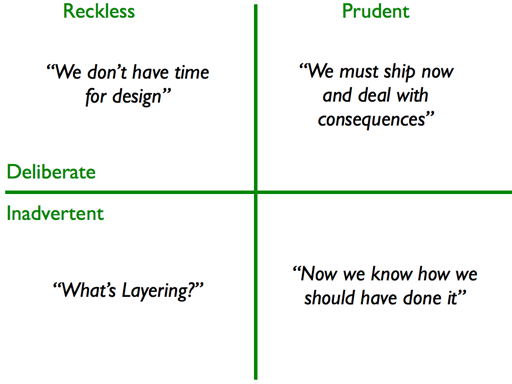
\includegraphics[width=80mm]{figures/chapter2/technicalDebtQuadrant}
	\caption{Technical Debt Quadrant}
	\label{fig:technical_debt_quadrant}
\end{figure}

\subsection{Other Insights on the Technical Debt Metaphor}

The technical debt metaphor has found favor with software developers who need to convey to project stakeholders uninitiated in programming terminology similar debts and patchwork repairs that ``kick the can down the road," temporarily delaying payment of outstanding money owed and putting off the effort of isolating a solution viable in the long term. Concepts falling under this umbrella include test and people debt, architectural and requirement debt and documentation and generalized software debt \cite{sterling2010managing}.

Broadening the metaphor to cover too many varieties of debt, however, might ultimately lessen its effectiveness, as Kruchten et al. point out \cite{Kruchten_td_IEEE}.  Unimplemented requirements, functions, or features do not qualify as requirement debts, just as putting off developing them does not qualify as a planning debt. Heavy reliance on tools alone to detect technical debt is one pitfall that the study highlights, in many cases leading to non-negligible underestimation of the actual technical debt load, since the majority of technical debt accumulates because of structural choices and technological gaps rather than code quality.

Further corroborating the overextension of the metaphor, Spinola et al. \cite{spinola2013investigating} compiled statements on technical debt that software developers made both online and in published work and selected 14 of them to use as items in two surveys measuring the level of agreement of 37 participants with software development backgrounds. On the whole, most participants strongly agreed that poorly managed technical debt drives up maintenance costs until they outpace consumer value and disagreed that all technical debt is accrued with a developer's full knowledge.

In the same study, the authors speculate that the technical debt metaphor's comprehensibility is what fuels its generalization to phenomena outside the realm of technical debt in the truest sense. This in turn blurs the boundaries between technical debt and other costs or coding flaws and leads to persistent conflation among non-technical project contributors and, all too often, industry specialists, who adopt the metaphor as an all-purpose catchall \cite{spinola2013investigating}.

Alves et al.\cite{alves2014towards} have introduced a specialized vocabulary intended to disambiguate the subtleties that a cover term such as "technical debt" overlooks, by sorting concepts extracted from a systematic literature mapping that combed 100 studies published between 2010 and 2014. Their undertaking identified 15 categories of technical debt but remained flexible enough to account for instantiations of technical debt that belonged in multiple categories: design debt, documentation debt, code debt, requirements debt, people debt, process debt, service debt, versioning debt, usability debt, build debt, test automation debt, infrastructure debt, defect debt, test debt, and architecture debt. The work of Alves et al. and others, who have monitored trends in the application of the technical debt metaphor and devised schemata relaying its latest interpretations, have allowed developers and their stakeholders to make sense of the dynamic interplay between holdover solutions and deferred expense.

\section{Technical Debt Indicators and Ramifications}


\subsection{Leveraging Source Code and Static Analysis Tools}

Lately, there has been a lot of incentive to engineer better strategies for detecting and managing technical debt. All too often technical debt gets out of hand and reaches unsustainable levels because a developer neglects to take stock as it accumulates. For all their limitations, static analysis tools do efficiently pinpoint source code anomalies and object-oriented violations outside the pre-specified ranges quantifying code quality. Such outliers constitute ``bad smells," which fall under the category of design debt.\\

In a study probing the effects of god classes (another manifestation of design debt) on project maintainability, Zazworka et al. \cite{zazworka2011investigating} examined two commercial applications released by a development company and concluded that god classes are more liable to be defective and thus higher-maintenance than non-god classes. For this reason, it is worthwhile for developers to monitor and, where appropriate, rein in the toll that technical debt takes on product quality, at all stages in the process.\\

God classes and other bad smells, namely, data class and duplicate code, were extracted from open source systems and scrutinized by Fontana et al.~\cite{fontana2013code} in an effort to prioritize handling different types of design debt. Their approach ranks bad smells in descending order with respect to negative impact on software quality and encourages developers to rectify higher-priority design debts first.\\

Zazworka et al. \cite{zazworka2011investigating} elicited an enumeration of technical debt items stored in project artifacts from multiple developers and compared the results with what three static analysis tools identified as fitting the relevant criteria. As different teams reported different technical debt items, consensus engenders underestimation of the actual technical debt load and aggregation proves to be the better method. Similarly, static analysis tools  will yield underestimations, some varieties of technical debt going undetected, unless supplemented with human mediation.

\subsection{Leveraging Source Code Comments (Self-Admitted Technical Debt)}

While strides have been made in locating sources of technical debt and preventing unsustainable accumulation, such as integrating tool- and developer-flagged code, new improvements are constantly proposed, debated, and adopted for use alongside older "tried and tested" methodologies. One such improvement, from Potdar and Shihab \cite{ICSM_PotdarS14} , enlists source code comments in isolating technical debt, the benefit of which is that the program developer \emph{confesses} the debt. At best, analysis tools can only \emph{suppose} debt on the basis of semi-arbitrary cutoffs and thresholds and stop short of guaranteeing that an implementation is less than optimal, i.e., \emph{self-admitted technical debt}.\\

In their pioneer study capturing the state-of-the-art in self-admitted technical debt identification, Potdar and Shihab \cite{ICSM_PotdarS14} extracted source code comments from five open source projects and conducted manual inspections. The authors read and analyzed more than 100,000 comments and in the end isolated 62 different comment patterns that serve as reliable indicators of self-admitted technical debt, most consisting of simple phrases along the lines of "fixme," "workaround," and "this can be a mess." It was found that (i) between 2.4 and 31.0\% of the files analyzed contained these keywords, (ii) the bulk of the self-admitted technical debt was introduced by more experienced developers and (iii) there is no correlation between time pressures or code complexity and the amount of self-admitted technical debt.\\

Building on the groundbreaking work of Potdar and Shihab \cite{ICSM_PotdarS14}, Bavota and Russo \cite{bavota2016large} considered the growth and evolution of self-admitted technical debt across 159 projects and the effects this has had on software quality, and extracted upwards of 600,000 commits and 2 billion source code comments. They found that (i) self-admitted technical debt is diffused, averaging 51 occurrences per system, (ii) it accumulates over time as new occurrences pile up on top of ones which have not yet been corrected and (iii) the occurrences that are corrected have a mean lifespan of 1,000 commits in the system.


\subsection{Research Leveraging Source Code Comments}


A number of studies examined the usefulness/quality of comments and showed that comments are valuable for program understanding and software maintenance \cite{TakangGM96,tan07icomment,lawrie2006leveraged}. For example, Storey \emph{et al.}~\cite{Storey:2008} explored how task annotations in source code help developers manage personal and team tasks. Takang {\em et al.} \cite{TakangGM96} empirically investigated the role of comments and identifiers on source code understanding. Their main finding showed that commented programs are more understandable than non-commented programs. Khamis {\em et al.} \cite{Khamis:2010} assessed the quality of source code documentation based on an analysis of the quality of language and consistency between source code and its comments. Tan {\em et al.} proposed several approaches to identify inconsistencies between code and comments. The first, called @iComment, detects lock- and call-related inconsistencies \cite{tan07icomment}. The second approach, @aComment, detects synchronization inconsistencies related to interrupt context \cite{acomment}. A third approach, @tComment, automatically infers properties from Javadoc related to null values and exceptions; it performs test case generation by considering violations of the inferred properties \cite{tcomment}.

Other studies have examined the co-evolution and reasons for comment updates. Fluri {\em et al.} \cite{fluri2007code} studied the co-evolution of source code and associated comments and found that 97\% of the comment changes are consistently co-changed. Malik {\em et al.}  \cite{malik2008understanding} performed a large empirical study to understand the rationale for updating comments along three dimensions: characteristics of the modified function, characteristics of the change, as well as the time and code ownership. Their findings showed that the most relevant attributes associated with comment updates are the percentage of changed call dependencies and control statements, the age of the modified function and the number of co-changed functions which depend on it. De Lucia {\em et al.} \cite{DeLucia2011} proposed an approach to help developers maintain source code identifiers and consistent comments with high-level artifacts. The main results of their study, based on controlled experiments, confirm the conjecture that providing  developers with similarity between source code and high-level software artifacts helps to enhance the quality of comments and identifiers.



Most relevant to our research is the recent work undertaken by Potdar and Shihab \cite{ICSM_PotdarS14}, which uses source code comments to detect self-admitted technical debt. Using the identified technical debt, they studied  how much SATD exists, the rationale for SATD, as well as the likelihood of its removal after introduction. Another relevant contribution to our study is Maldonado and Shihab's \cite{MTD15p9}, as their work has also leveraged source code comments to detect and quantify different types of SATD. They classified SATD into five types:  design debt, defect debt, documentation debt, requirement debt and test debt. Ultimately, they concluded that  the  most common type is design debt, accounting for anywhere between 42\% and 84\% of a total of 33K classified comments.

Our study builds on the prior work in~\cite{ICSM_PotdarS14,MTD15p9} since we use the comment patterns they produced to detect SATD. However, in a departure from their studies, we examine the relationship between SATD and software quality.


\subsection{Technical Debt}

Other work has focused on the identification and examination of technical debt. It is important to note that the technical debt discussed here is \emph{not} SATD: rather it is technical debt that is detected through source code analysis tools. For example,  Zazworka {\em et al.} \cite{Zazworka:2013} attempted to identify technical debt automatically and then compared their automated identification with human elicitation. The results of their study outline potential benefits of developing tools and heuristics for the detection of technical debt. Also, Zazworka {\em et al.} \cite{zazworka2011investigating} investigated how design debt, in the form of god classes, affects software maintainability and correctness of software products. Their study involved two industrial applications and showed that god classes are changed more often than non-god classes and, moreover, that they contain more defects. Their findings suggest that technical debt may negatively influence software quality. Guo {\em et al.}~\cite{GuoSGCTSSS11} analyzed how and to what extent technical debt affects software projects by tracking a single delayed task in a software project throughout its lifecycle. As discussed earlier, the work by Potdar and Shihab \cite{ICSM_PotdarS14} is also related to our work, which differs from precedent primarily in that it focuses on SATD.


Our work differs from foregoing research by Zazworka {\em et al.}~\cite{zazworka2011investigating,Zazworka:2013} since we focus on the relationship between SATD (and not technical debt related to god files) and software quality. However, we believe that our study complements prior studies since it sheds light on the overall impact of SATD and, in particular, its ramifications for software quality.



\subsection{Software Quality}

A plethora of prior work has proposed techniques to improve software quality, the majority of this work having concerned itself with understanding and predicting software quality issues (e.g.~\cite{Zimmerman2008Springer}). Several studies have examined the metrics that best indicate software defects, including design and code~\cite{Jiang-promise-2008}, code churn~\cite{Nagappan-icse-2005}, and process metrics~\cite{Moser-icse-2008,Rahman-icse-2013}.

Other studies have opted to focus on change-level prediction of defects. Sliwerski  \emph{et al.} suggested a technique known as SZZ to automatically locate fix-inducing changes by linking a version archive to a bug database \cite{Sliwerski-fse-2005}.   Kim \emph{et al.} \cite{Kim-tse-2008} used identifiers in added and deleted source code and the words in change logs to identify changes as defect-prone or not. Similarly,  Kamei \cite{Kamei-tse-2013} proposed a  ``Just-In-Time Quality Assurance''  approach to identify risky software changes in real time.  The findings of their study reveal that process metrics outperform product metrics in terms of identifying risky changes.

Our study leverages the SZZ algorithm and some of the techniques presented in the aforementioned change-level work to study the defect-proneness of SATD-related commits. Moreover, our study complements existing work by taking up the hypothetical correlation between SATD and software defects.


\chapter{Examining the Impact of Self-Admitted Technical Debt on Software Quality}
\label{chapter3}
% -*- root: cuthesis_masters.tex -*-

\section{Introduction}
\label{chap3:sec:introduction}
Software companies and organizations have a common goal when developing software projects: both aim to deliver high-quality, useful software in a timely manner. However, in most practical settings, developers and development companies are saddled with deadlines, giving them every incentive to release earlier than the ideal date, were product quality alone taken into account. Such situations are all too common and in many cases force developers to take shortcuts \cite{kruchten2013technical} \cite{seaman2015technical}. Recently, the term \emph{technical debt} was coined to denote the phenomenon of ``doing something that is beneficial in the short term but will incur a cost later on''~\cite{cunningham1993wycash}. Prior work has shown that practitioners cite numerous reasons for assuming technical debt, among them: rushing to compensate for delays and still deliver on time or to make deadlines for incorporating with a partner product before release, alleviating time-to-market pressure and meeting customer demands in a time-sensitive industry~\cite{lim2012balancing}.


% People studied different aspects of TD
More recently, a study by Potdar and Shihab \cite{ICSM_PotdarS14} introduced a novel method of identifying technical debt reported by developers. This so-called ``self-admitted technical debt," abbreviated SATD, is declared in developer source code comments. Prior work \cite{MTD15p9} has demonstrated that accrual of SATD is commonplace in software projects, where reviewing source code comments can identify different types of technical debt (e.g. design, defect and requirement debt).

Intuition and general belief concur that inducing a technical debt, which many developers resort to in a time crunch, negatively impacts software maintenance and overall quality~\cite{zazworka2011investigating,spinola2013investigating,GuoSGCTSSS11,seaman2015technical,kruchten2013technical}. However, to the best of our knowledge, there is no empirical study that examines the impact of SATD on software quality. Such a study is critical since it will help us to confirm or refute entrenched preconceptions regarding the technique and better understand how to manage SATD.


Therefore, in this chapter, we investigate the empirical relation between SATD and software quality in five open-source projects. In particular, we examine whether (i) files with SATD have more defects compared to files without SATD, (ii) whether SATD changes introduce more future defects and (iii) whether SATD-related changes tend to be more difficult. We measured the difficulty of a change in terms of the amount of churn, number of files, number of modified modules, and change entropy. Our findings show that: i) while it is true that SATD files have more bug-fixing changes in a number of the studied projects, in other projects, files without SATD have more defects, thus there is no clear relationship between defects and SATD; ii) SATD changes are associated with less future defects than non-SATD changes and iii) SATD changes (i.e., changes touching SATD files) are more difficult to perform. Our study indicates that although technical debt has negative effects, its impact is not related to defects, but rather to making the system more difficult to change in the future.


\section{Related Work}
\label{chap3:sec:related_work}
Our work focuses on \SATD, which analyzes comments to detect technical debt, we discuss the work related to three main topics: (i) source code comments, (ii) technical debt, and (iii) software quality.

\subsection{Source Code Comments}
The well-attested utility of source code comments rests on facilitation of personal and team task management as well as the greater understandability of commented programs relative to uncommented programs \cite{lawrie2006leveraged, Storey:2008, TakangGM96,tan07icomment}. Source code comment quality, meanwhile, depends in large part on code-comment consistency, which developers optimize when they revise comments and code in tandem. Three techniques that Tan \textit{et al.} advocate for detection of code-comment inconsistencies are @iComment, @aComment and @tComment---specialized to detect lock- and call-related, interrupt context synchronization and inferred property violation inconsistencies, respectively \cite{tan07icomment, acomment, tcomment}. Nonetheless, a study by Fluri \textit{et al.} put the co-change (code-comment consistency) rate at 97\%

As for the impetuses that compel developers to revise source code comments in the first place, the work of Malik \textit{et al.}~\cite{malik2008understanding} points to the share of changed call dependencies and control statements, the age of the modified function and the number of co-changed dependent functions. In another study, De Lucia \textit{et al.}~\cite{DeLucia2011} offered proof that correspondence between source code and high-level software artifacts is beneficial both in terms of comment quality and reliability of source code identifiers.

Another factor contributing to the utility of source code comments is how amenable they are to the identification of \SATD, which Potdar and Shihab~\cite{ICSM_PotdarS14} took advantage of in determining how widespread the phenomenon of SATD is, why developers resort to it and at what rate it is removed once introduced. In addition, Maldonado and Shihab~\cite{MTD15p9} employed source code comments to categorize \SATD and determine the relative incidence of each variety: 13,800 to 27,800 of the 33,000 comments inspected turned out to be attributable to design debt---the most common SATD category.

\subsection{Technical Debt}
Other types of technical debt, i.e. technical debt identified by source code analysis tools, has attracted its own research. Comparing automated and manual detection methods, Zazworka \textit{et al.}~\cite{Zazworka:2013} concluded that it would behoove the software development community to build additional tools and innovate heuristics for the express purpose of detecting technical debt. In another study, Zazworka \textit{et al.}~\cite{zazworka2011investigating} assessed the effect of god class design debt on long-term software maintenance and found that god classes are more change-prone and defective than non-god classes, suggesting that technical debt adversely impacts software quality. Zooming in on the lifecycle of one delayed task, Guo \textit{et al.}~\cite{GuoSGCTSSS11} figured out in what ways these adverse effects manifest themselves in individual software projects.

\subsection{Software Quality}
Much foregoing work has sought to improve software quality by enumerating and forecasting software quality issues and threats, e.g.~\cite{Zimmerman2008Springer}. Other work has honed in on defect indicator metrics, among them: design and code~\cite{Jiang-promise-2008}, code churn~\cite{Nagappan-icse-2005} and process metrics~\cite{Moser-icse-2008,Rahman-icse-2013}.

Yet change-level defect prediction has been steadily gaining ground, with Sliwerski \textit{et al.}'s SZZ algorithm, which locates fix-inducing changes by linking a version archive to a bug database~\cite{Sliwerski-fse-2005}, and Kim \textit{et al.}'s~\cite{Kim-tse-2008} modified source code and change log identifiers of defect-proneness. Additionally, the ``Just-In-Time Quality Assurance" approach developed by Kamei~\cite{Kamei-tse-2013} flags risky software changes. It was found that process metrics are better at identifying risky changes than product metrics.

\section{Approach}
\label{chap3:sec:approach}

The objective of our study is to investigate the relationship between SATD and software quality. We measure software quality in two ways. First, we employ the traditional measure of counting the defects in a file and defect-inducing changes, which is in line with most prior studies ~\cite{Kamei-tse-2013,Kim-tse-2008,sliwerski-msr-2005}. In particular, we measure the number of defects in SATD-related files and the percentage of SATD-related changes that introduce future defects. Second, since technical debt is meant to represent the phenomenon of taking a short-term benefit at the cost of paying a higher price later on, we employ as another measure the difficulty of the changes related to SATD. Specifically, we use amount of churn, number of files, number of directories and change entropy to quantify difficulty. We formalize our study with the following three research questions:


\begin{itemize}
	\vspace{0.2cm}
	\item {\bf RQ1:} Do files containing SATD have more defects than files without SATD? Do the SATD files have more defects after the introduction of SATD?\\
	%\vspace{0.2cm}
	\item {\bf RQ2:} Do SATD-related changes introduce future defects?\\
	%\vspace{0.2cm}
	\item {\bf RQ3:} Are SATD-related changes more difficult than non-SATD changes?
	%\vspace{0.2cm}
\end{itemize}


To address our research questions, we followed the general procedure enumerated in Figure \ref{fig:Process_overview}, which consists of the following steps. First, we mined the source code repositories of the studied projects (step 1). Then, we extracted  source code files at the level of each analyzed project (step 2). Next, we parse the source code and extract comments from the source code of the analyzed systems (step 3). At this point, we apply the comment patterns proposed by Potdar and Shihab~\cite{ICSM_PotdarS14} to identify SATD (step 4). Finally, we analyze the changes to quantify defects in files and use the SZZ algorithm to determine defect-inducing changes (step 5).

%and then linking them to the issue-tracker systems (steps 6). Finally, we generated the results and discussed them in detail (step 7).

\begin{figure}[t]
	\centering
	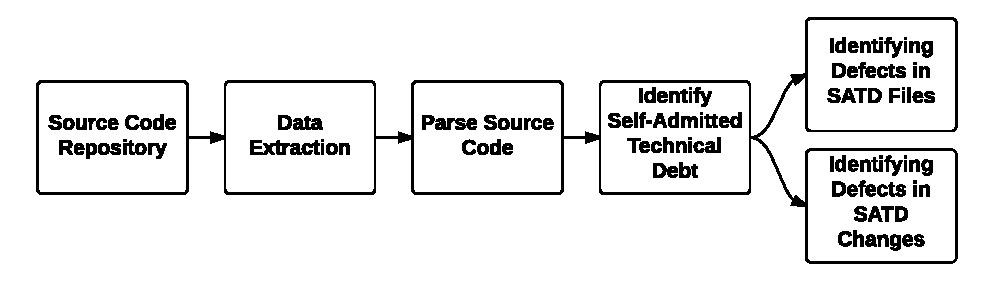
\includegraphics[width=150mm]{figures/chapter3/approach}
	\caption{Approach overview.}
	\label{fig:Process_overview}
\end{figure}


\subsection{Data Extraction}
Our study analyzes five large open-source software systems---namely Chromium, Hadoop, Spark, Cassandra and Tomcat. We chose these projects because they represent different domains and programming languages (\ie{}, Java, C, C++,  Scala, Python and Javascript) and have a large number of contributors. More importantly, these projects are well-commented (since our approach for the detection of SATD is based on source code comments). Moreover, they are all available to the research community as well as industry practitioners and have considerable development history.

Our analysis requires the source code as input. We downloaded the latest publicly available releases of the systems under consideration, \ie{}, Chromium, Hadoop, Spark, Cassandra and Tomcat. Then, we filtered the data to extract the source code at the level of each project release. Files not consisting of source code (\eg{} CSS, XML, JSON) were excluded from our analysis as they do not contain the comments our analysis relies on.\\

Table~\ref{table:projects_statistics} summarizes the main characteristics of these projects. It reports for each: (i) the relevant project release, (ii) the date of the release, (iii) the number of lines of code, (iv)  the number of comment lines, (v)  the number of source code files, (vi)  the number of committers and (vii) the number of commits.

%\begin{landscape}
	
\begin{table*}[t]

		%\def\arraystretch{1.5}%

		\centering
		\caption{Characteristics of the studied projects.}
				\begin{adjustbox}{width=1.0\textwidth}
		\begin{tabular}{l|ll|ccccc}
			\hline
			\textbf{Project}  & \textbf{Release} & \textbf{ Release Date}  & \textbf{\# Lines of Code} & \textbf{\# Comment Lines} & \textbf{\# Files} & \textbf{\# Committers} & \textbf{\# Commits} \\ \hline
			\textbf{Chromium} &   45    & Jul 10, 2015 &  9,388,872   &    1,760,520    & 60,476 &    4,062    & 283,351  \\ \hline
			\textbf{Hadoop} &   2.7.1    & Jul 6, 2015 &  1,895,873   &    378,698    & 7,530 &    155    & 11,937  \\ \hline
			\textbf{Spark} &   2.3    & Sep 1, 2015 &  338,741   &    140,962    & 2,822 &    1,056    & 13,286  \\ \hline
			\textbf{Cassandra} &   2.2.2    & Oct 5, 2015 &  328,022   &    72,672    & 1,882 &    219    & 18,707  \\ \hline
			\textbf{Tomcat} &   8.0.27    & Oct 1, 2015 &  379,196   &    165,442    & 2,747 &    34    & 15,914  \\ \hline
		\end{tabular}
		\label{table:projects_statistics}
	\end{adjustbox}
\end{table*}

%\end{landscape}

\subsection{Scanning Code and Extracting Comments}
After obtaining the source code of the five software projects, we extracted the comments from their source code files. To this end, we developed a Python-based tool that identifies comments based on the use of regular expressions. This tool also indicates comment type (\ie{}, single-line or block comments), the name of the file where the comment appears and the line number of the comment. To ensure our tool's accuracy, we employ the Count Lines of Code (CLOC) tool~\cite{cloc}. As long as the total number of lines of comments is the same according to both tools, then the tool we developed can be considered independently reliable.

In total, we found 879,142 comments for Chromium; 71,609 for Hadoop; 31,796 for Spark; 20,310 for Cassandra and 39,024 for Tomcat. Of these, SATD comments numbered 18,435 for Chromium; 2,442 for Hadoop; 1,205 for Spark; 550 for Cassandra and 1,543 for Tomcat. To enable easy processing, we store all of our processed data in a PostgreSQL database, which we query to answer our RQs.


\subsection{Identifying Self-Admitted Technical Debt}
\label{td}
To perform our analysis, we need to identify \SATD at two levels: (i) the file level and (ii) the change level.



\noindent\textbf{SATD files:} To identify SATD, we followed the methodology outlined in Potdar and Shihab~\cite{ICSM_PotdarS14}, who generated a list of 62 different patterns that indicate SATD. Therefore, in our approach, we determine which comments identify SATD by locating those that match any of the 62 patterns associated with SATD. These patterns are extracted from several projects and some appear more often than others. Examples of these patterns include: ``\textit{hack, fixme, is problematic, this isn't very solid, probably a bug, hope everything will work, fix this crap}." The complete list of the patterns considered in this study is available online\footnote{http://users.encs.concordia.ca/\textasciitilde eshihab/data/ICSME2014/data.zip}.

Once we identify the comment patterns, we then abstract up to determine the SATD files. Files containing at least one of the SATD comments are then labeled as {\em SATD files}, while files that do not contain any of these SATD comments are referred to as {\em non-SATD files}. We use these SATD files to answer RQ1.

\noindent\textbf{SATD changes:}
To study the impact of SATD at the change level, we need to identify SATD changes on the basis of the SATD files just identified. We analyze the changes and determine all the files that were touched by each change. If at least one of the files touched by the change is an SATD file, then we label that particular change as an SATD change. If the change does not touch any SATD files, then we label it as a non-SATD change. Table~\ref{table:satd_analyzed_projects} displays the percentage of SATD comments and files for each of the studied systems. From the table, we see that SATD comments exhaust less than 4\% of the total comments, and between 10.17\% and 20.14\% of the files are SATD files.

\begin{table}[tbh]
	\setlength{\tabcolsep}{.7\tabcolsep}
	\centering
	\caption{Percentage of SATD of the analyzed projects.}
	\begin{tabular}{l|c|c}
		\hline
		\textbf{Project}   & \textbf{SATD Comments (\%)} & \textbf{SATD files (\%)} \\ \hline
		\textbf{Chromium}  & 2.09             & 10.43                             \\ \hline
		\textbf{Hadoop}    & 3.41             & 18.59                             \\ \hline
		\textbf{Spark}     & 3.79             & 20.14                             \\ \hline
		\textbf{Cassandra} & 2.70             & 16.01                             \\ \hline
		\textbf{Tomcat}    & 3.95             & 10.17                             \\ \hline
	\end{tabular}
	\label{table:satd_analyzed_projects}
	\vspace{-0.2cm}
\end{table}
%\latifa {Did we apply SZZ, if yes we need a section on that as well - It is not clear whether it has been used or not}


\subsection{Identifying Defects in SATD Files and SATD Changes}
\label{bugs}
To determine whether a change fixes a defect, we search for co-occurrences of defect identifiers in change logs from the Git Version control system using regular expressions like ``\textit{fixed issue \#ID, bug ID, fix, defect, patch, crash,  freeze, breaks, wrong, glitch, properly, proper}."
Sliwersky \textit{et al.}~\cite{sliwerski-msr-2005} showed that the use of such keywords in the change logs usually indicates the correction of a mistake or failure.
A similar  approach  was applied  to  identify  fault-fixing  and
fault-inducing  changes in  prior work~\cite{Kamei-tse-2013,Kim-tse-2008, sliwerski-msr-2005}. Once this step is performed, we identify, for each defect ID, the corresponding defect report from
the corresponding issue tracking system, \ie{}, Bugzilla\footnote{https://www.bugzilla.org} or JIRA\footnote{https://www.atlassian.com/software/jira}, and extract the relevant information from each report.

After grouping the SATD files and SATD changes, we proceed to identify the defects each contains. To do so, we follow the protocol previous research has adhered to in determining the number of defects in a file and locating defect-inducing changes~\cite{Kamei-tse-2013,Kim-tse-2008, sliwerski-msr-2005}.

\noindent\textbf{Defects in files:} Comparing the defectiveness of SATD and non-SATD files hinges on having the number of file defects at our disposal. To ensure this, we extract all the changes that have touched a file throughout the system's entire history. Then, we search for keywords in the change logs that indicate defect-fixing, as demonstrated in Figure~\ref{fig:indicating-a-bug-fixing-change}. A subset of the keywords we entered contains: ``\textit{fixed issue \#ID, bug ID, fix, defect, patch, crash, freeze, breaks, wrong, glitch, proper}." In cases where a defect identification is specified, we extract the defect report to verify that the defect corresponds to the system (\ie{}, product).

Second, we establish whether the issue IDs identified in the change logs are true positives. Once we determine the defect-fixing changes, we use these changes as an indication of the defect fixes that occur in a file, i.e., we count the number of defects in a file as the number of defect-fixing changes.


\noindent\textbf{Defect-inducing changes:} Similar to the process above, we first determine whether a change fixes a defect. To do so, we use regular expressions and specific keywords referencing a fix to search the change logs (i.e., commit messages) from the source code control versioning system. In particular, we search for the following keywords: ``\textit{fixed issue \#ID, bug ID, fix, defect,  patch, crash, freeze, breaks, wrong, glitch, proper}." We also search for the existence of defect identification numbers in order to determine which defects, if specified, the changes actually fix.

Once we identify the defect-fixing changes, we map back (using the \texttt{blame} command) to determine all the changes that altered the fixed code in the past. We take the defect-inducing change to be the change that is closest to but still before the defect report date. In essence, this tells us that this was the last change before a defect showed up in the code. If no defect report is specified in the fixing change, then following the precedent of prior work~\cite{Kamei-tse-2013}, we assume that the last change before the fixing change was the change that introduced the defect. This approach is often referred to as the SZZ~\cite{sliwerski-msr-2005} or approximate (ASZZ) algorithm~\cite{Kamei-tse-2013} and is to date the state of the art in identifying defect-inducing changes.


\begin{figure}[h]
	\centering
	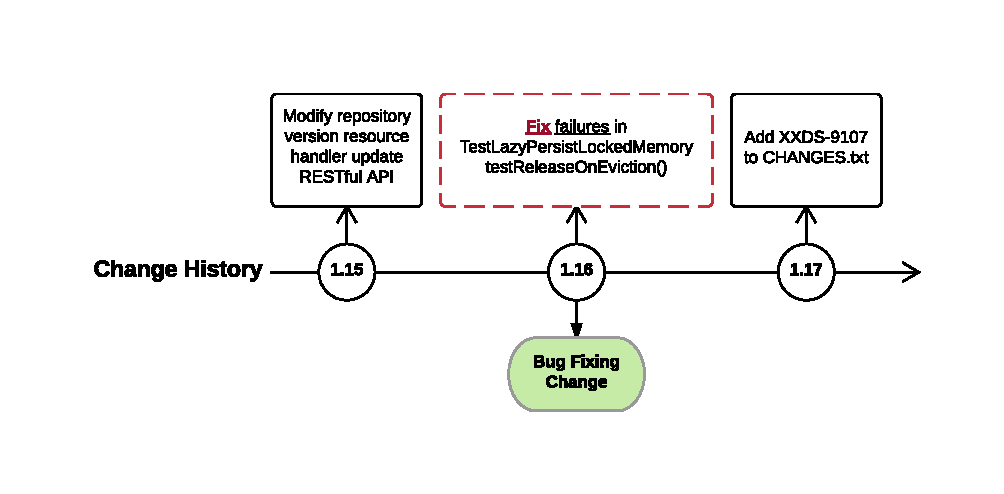
\includegraphics[width=150mm]{figures/chapter3/bug-fixing-change}
	\caption{Indicating a bug-fixing change.}
	\label{fig:indicating-a-bug-fixing-change}
\end{figure}



\section{Mann-Whitney-Wilcoxon Rank Sum Test}
The Mann-Whitney-Wilcoxon Rank Sum Test is used to analyze the differences between two groups of the same attribute for a data set~\cite{mann1947test}. This statistical test makes use of median values for its comparison rather than mean values, allowing it to characterize populations that do not follow a normal curve distribution. The main result of the test is the \textit{p}-value it generates, which quantifies the probability of the null hypothesis being true, with the null hypothesis in this case being that both groups have the same central tendency. In our study we use this test to determine if the distinction between SATD and non-SATD files results in a difference in relevant statistical properties. If it does, then whatever caused a noticeable distinction between the file categories is meaningful to the statistical property. 




\section{Case Study Results}
\label{chap3:sec:results}

\begin{figure}[tb]
	\centering
	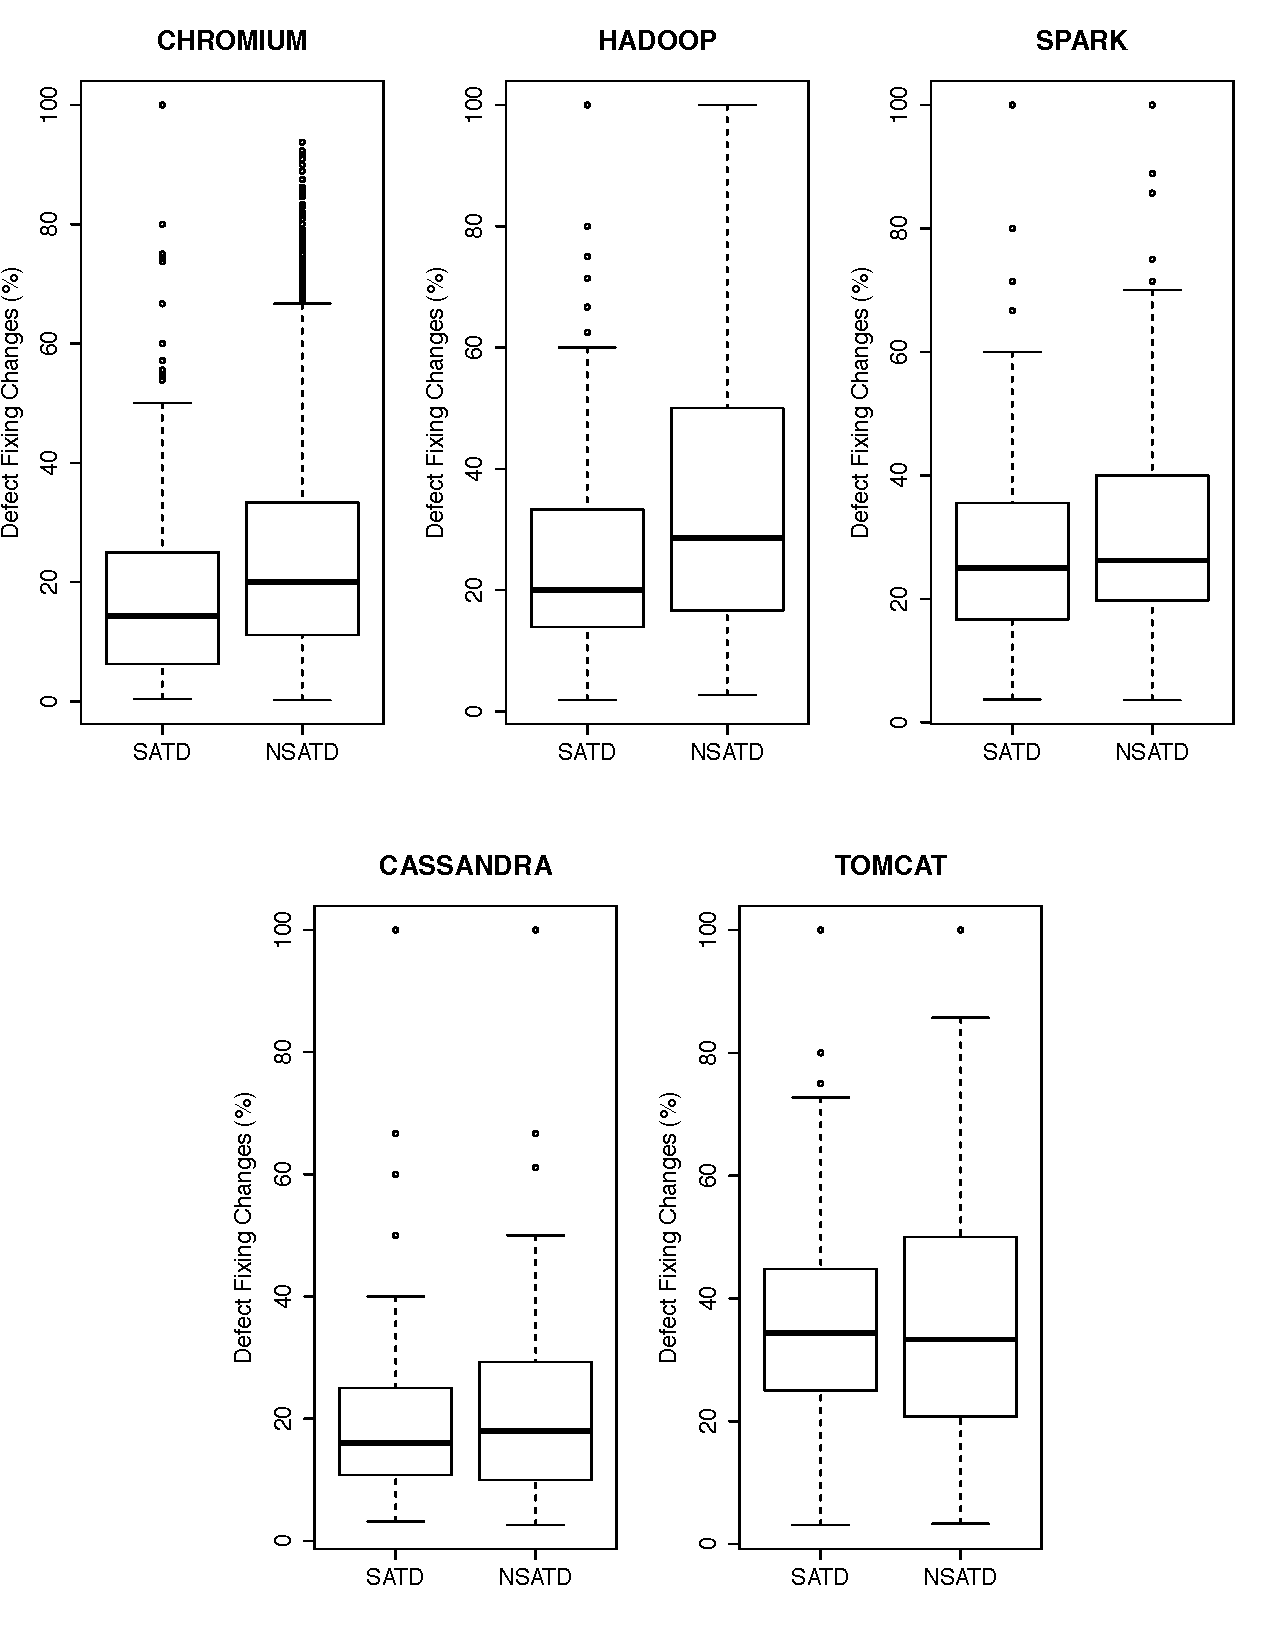
\includegraphics[width=90mm]{figures/chapter3/rq1_correction}
	\caption{Percentage of defect-fixing changes for SATD and NSATD files.}
	\label{figure:number_of_fixing_changes_TD_vs_NTD}
\end{figure}

This section reports the results of our empirical study examining the relationship between self-admitted technical debt and software quality. 

For each project, we provide the descriptive statistics and statistical results, as well as a comparison with the other projects. 



In what follows, we present for each RQ its motivation, the approach we took to address it and our findings.


\subsection*{RQ1: Do files containing SATD have more defects than files without SATD? Do the SATD files have more defects after the introduction of SATD?}

\noindent{\textbf{Motivation:}} Intuitively, technical debt has a negative impact on software quality. Researchers have studied technical debt and shown that it negatively impacts software quality~\cite{zazworka2011investigating}. However, this research has neglected SATD, which is prevalent in software projects according to past research \cite{ICSM_PotdarS14}.

Empirically examining the impact of SATD on software quality provides researchers and practitioners with a better global understanding of the phenomenon, warns them of its future risks and raises awareness of the obstacles or challenges it can pose.

In addition to comparing the defect-proneness of SATD and non-SATD files, we compare the defect-proneness of SATD files before (pre-SATD) and after SATD (post-SATD). This analysis provides us with a different view of the defect-proneness of SATD files and, in essence, tells us whether the introduction of SATD is at all related to the defects we observe.



\begin{figure}[tb]
	\centering
	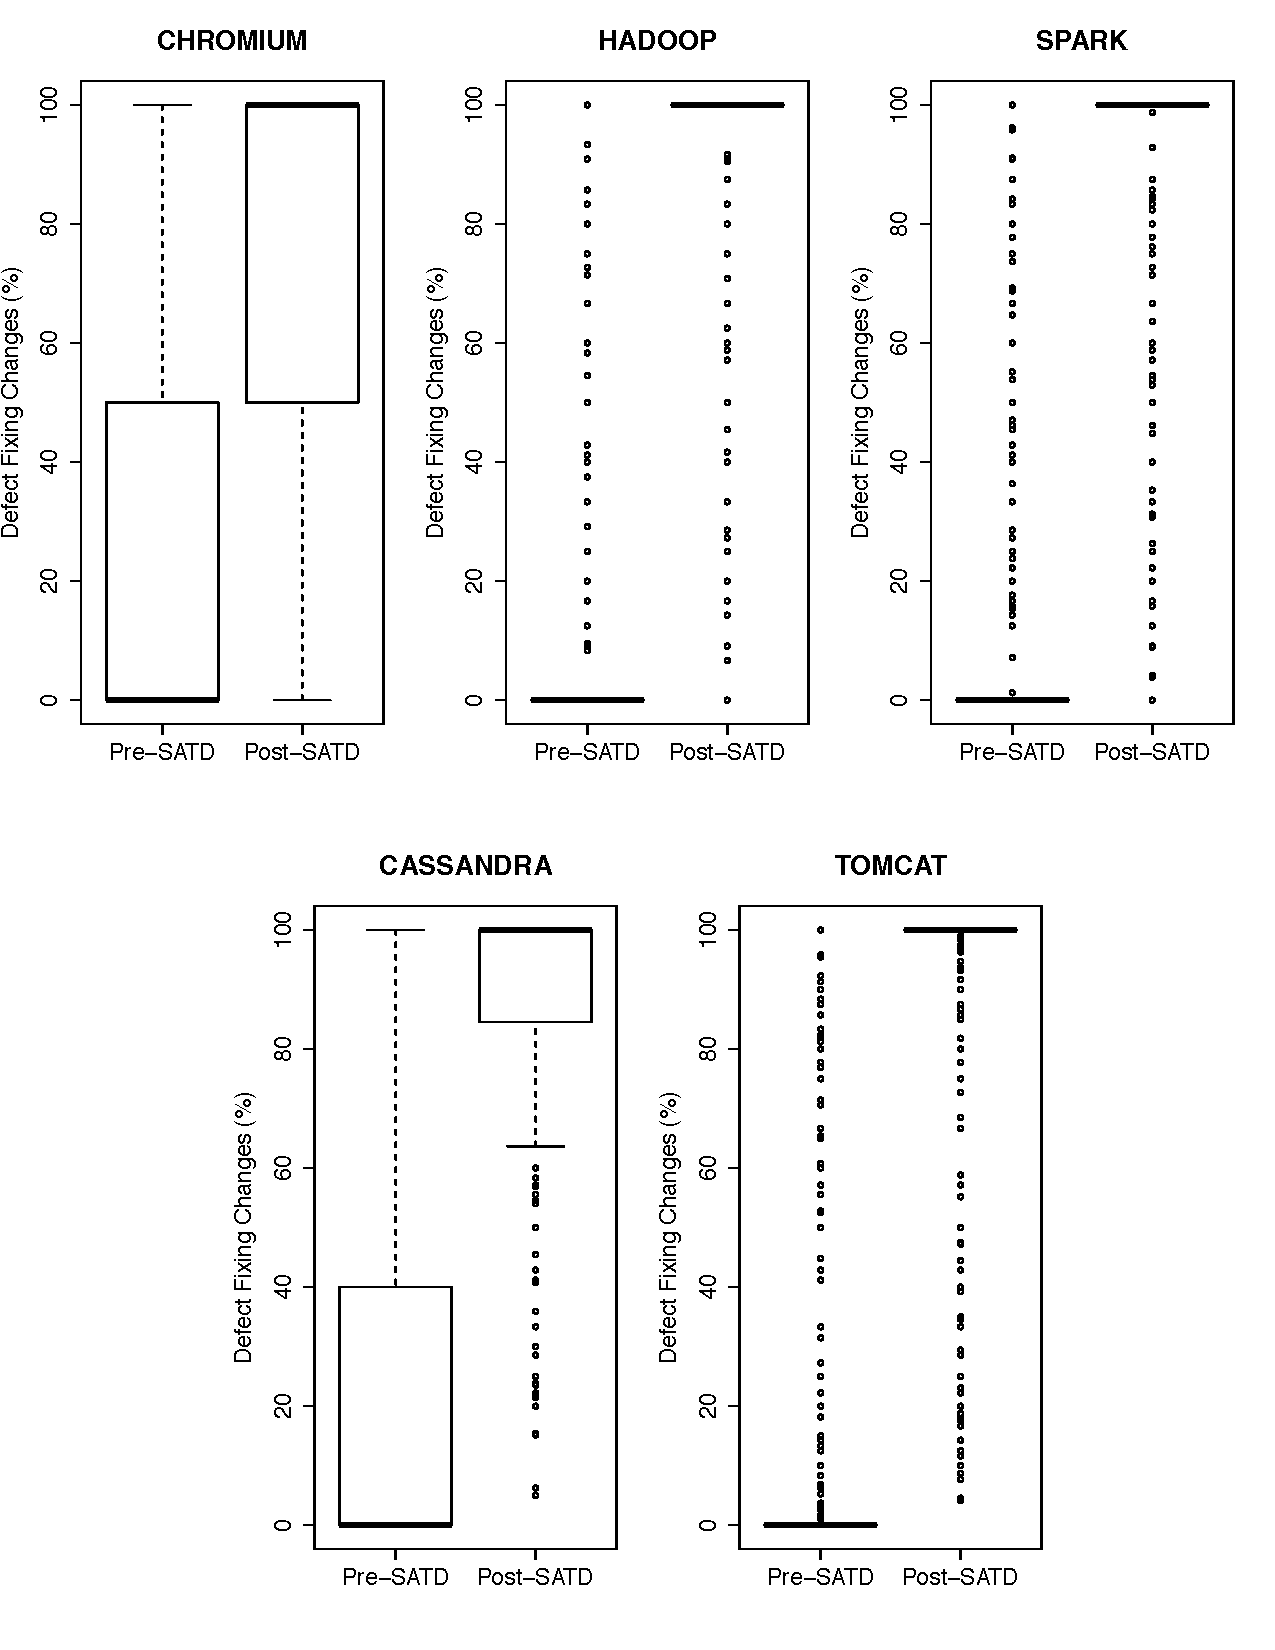
\includegraphics[width=90mm]{figures/chapter3/rq1-2_correction}
	\caption{Percentage of defect fixing changes for  pre-SATD and post SATD.}
	\label{figure:preVpost}
\end{figure}

\noindent{\textbf{Approach:}} To address RQ1, we perform two types of analyses. First, we compare the defect-proneness of files that do and do not contain SATD. Second, for the SATD files only, we compare defect-proneness before and after the introduction of SATD.

\noindent\textbf{Comparing SATD and non-SATD files.} To perform this analysis, we follow the procedure for identifying SATD files summarized earlier in section~\ref{td}. In a nutshell, we determine which files contain at least one SATD comment and label them as SATD files. Files that do not contain any SATD are labeled as non-SATD files. Once we sort the files, we determine the percentage of defect-fixing changes in each file category (SATD and non-SATD). We opt for percentages over raw numbers so as to normalize our data, since files can have different amounts of changes. To answer the first part of RQ1, we plot the distribution of defects by file category and perform statistical tests to compare the differences.

We perform the Mann-Whitney~\cite{mann1947test} test to determine if a statistical difference exists between the categories and Cliff's delta~\cite{Cliff:2005} to compute the effect size. We use the Mann-Whitney test instead of other statistical difference tests because it is a non-parametric test that accommodates non-normal distribution (and as we will see later, our data is not normally distributed). We consider the results of the Mann-Whitney test to be statistically significant if the \textit{p}-value is such that $p <= 0.05$. In addition, we compute the effect size of the difference using the Cliff's delta ($d$) non-parametric effect size measure, which measures how often values in one distribution are larger than the values in another. Cliff's $d$ ranges in  the interval $[-1,1]$ and is considered small for $0.148 \le d < 0.33$, medium for $0.33 \le d < 0.474$ and large for $d \ge 0.474$.




\noindent\textbf{Comparing files pre- and post-SATD.} To compare SATD files pre- and post-SATD, we first determine all the changes that touched a file and then identify the change that introduced the SATD. Next, we measure the percentage of defects (i.e., $\frac{\#~of~fixing~changes}{total~\#~changes}$) in the file before and after the introduction of the SATD. We compare percentage of defects instead of raw numbers since SATD could be introduced at different times, i.e., we may not have the same total number of changes before and after the SATD-inducing change. Once we determine the percentage of defects in a file pre- and post-SATD, we perform the same statistical test and effect size measure, \ie{}, Mann-Whitney and Cliff's delta.


\noindent{\textbf{Results - Defects in SATD and non-SATD files:}} Figure \ref{figure:number_of_fixing_changes_TD_vs_NTD} shows the percentage of defect-fixing changes in SATD and non-SATD files for the five projects. We observe that in four out of five cases, the non-SATD (NSATD) files have a slightly higher percentage of defect-fixing changes---in Chromium, Hadoop, Spark and Cassandra. However, in Tomcat, SATD files have a slightly higher percentage of defects. For all projects, the $p$-values were such that $p < 0.05$, indicating that the difference is statistically significant. However, when we closely examine the Cliff's delta values in Table~\ref{table:cliff_deltas_RQ1}, we see a different trend for Chromium. In Chromium and Tomcat, SATD files often have higher defect percentages than non-SATD files and the effect size is medium for Chromium and small for Tomcat. On the other hand, in Hadoop, Cassandra and Spark, SATD files have lower defect percentages than non-SATD files and this effect is large for Hadoop, medium for Cassandra and small for Spark.

Our findings here underscore that there is no clear trend when it comes to the percentage of defects in SATD versus non-SATD files. In some projects, SATD files have more bug-fixing changes, while in others, it is the non-SATD files that have a higher percentage of defects.

\begin{table}[tb]
	\setlength{\tabcolsep}{.7\tabcolsep}
	\centering
	\caption{Cliff's Delta for SATD versus NSATD and POST versus PRE fixing changes.}
	\begin{tabular}{l|c|c}
		\hline
		\textbf{Project}   & {\bf SATD vs. NSATD} & {\bf Post- SATD vs. Pre- SATD} \\ \hline
		\textbf{Chromium}  & 0.407          & 0.704        \\ \hline
		\textbf{Hadoop}    & -0.562         & 0.137        \\ \hline
		\textbf{Spark}     & -0.221         & 0.463        \\ \hline
		\textbf{Cassandra} & -0.400         & 0.283        \\ \hline
		\textbf{Tomcat}    & 0.094          & 0.763        \\ \hline
	\end{tabular}
	\label{table:cliff_deltas_RQ1}
\end{table}

\noindent{\textbf{Results - Defects in SATD files, pre- and post-SATD:}} Figure~\ref{figure:preVpost} shows boxplots for the percentage of defect-fixing changes in SATD files, pre- and post-SATD. Unsurprisingly, the post-SATD percentage of defect-fixing changes is higher for all projects. In Table~\ref{table:cliff_deltas_RQ1}, the effect size Cliff's delta values corroborate our visual observations in that there is again more defect-fixing in the SATD files post-SATD than pre-SATD. For all projects except Hadoop and Cassandra, where effect size is small, the Cliff's delta is large.
%\latifa {any clues from the data or previous experience why this could be the case?}.


These findings contend that although it is not always clear whether SATD or non-SATD files will have a higher percentage of defects, there is a consistently higher percentage of defect-fixing once SATD has been introduced.



\begin{figure}[tb!]
	\centering
	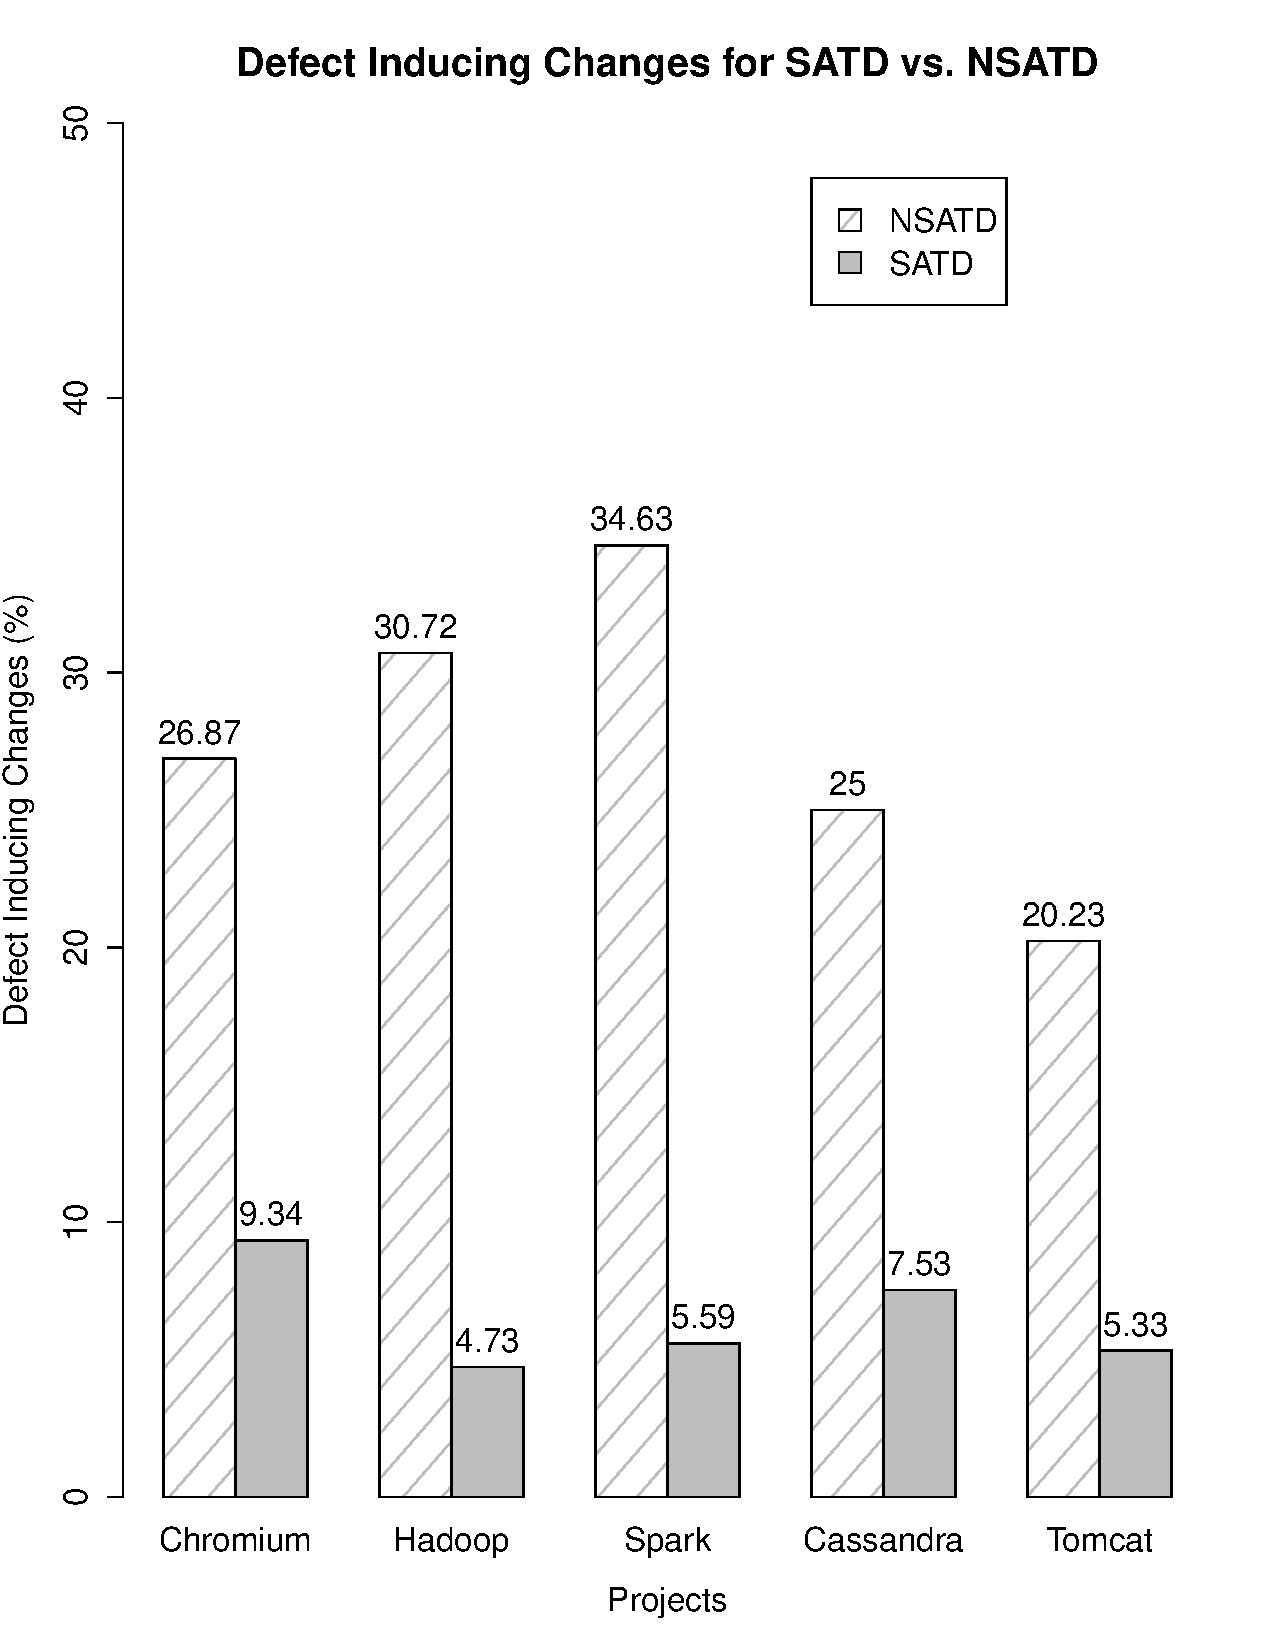
\includegraphics[width=90mm]{figures/chapter3/bug_inducing_changes}
	\caption{Percentage of defect inducing changes with SATD and NSATD.}
	\label{figure:bug_inducing_changes}
\end{figure}

\subsection*{RQ2: Do SATD-related changes introduce future defects?}

\noindent{\textbf{Motivation:}} After investigating the relationship between SATD and non-SATD at the file level, we would like to conclude whether SATD changes are more likely to introduce future defects. Whereas the file-level analysis looked at files as a whole, our analysis here is more fine-grained and tailored to assess individual changes.

Studying the propensity of SATD changes to introduce future defects is important, as it informs us as to how SATD and non-SATD changes compare in terms of future introduction of defects and how quickly the impact of \SATD on quality can be felt. For example, if SATD changes introduce defects in the very next change, then this tells us that there is essentially no latent stage and the impact of SATD is felt almost immediately. Our conjecture is that SATD changes tend to be more complex and lead to the introduction of defects.


\noindent{\textbf{Approach:}}
To address RQ2, we applied the SZZ algorithm~\cite{sliwerski-msr-2005} in order to detect defect-inducing changes. Then, we sorted the results into two categories: SATD and non-SATD defect-inducing changes.




\noindent{\textbf{Results:}}
Figure \ref{figure:bug_inducing_changes} demonstrates that non-SATD changes have a higher incidence of defect-inducing changes relative to SATD changes.  In Chromium, for example, roughly 10\% of the SATD changes induce future defects, compared to about 27\% of the non-SATD changes. Our findings here show that contrary to our conjecture, SATD changes actually have a lower chance of inducing future defects.




\begin{table}[tb!]
	\setlength{\tabcolsep}{.7\tabcolsep}
	\centering
	\caption{Cliff's Delta for the change difficulty measures across the projects.}
	\begin{tabular}{l|C{1.5in}|c|c|C{2in}}
		\hline
		\textbf{Project}   & {\bf \# Modified Files}    & {\bf Entropy} & {\bf Churn} & {\bf\# Modified Directories}    \\ \hline
		\textbf{Chromium}  & 0.418 & 0.418   & 0.386 & 0.353 \\ \hline
		\textbf{Hadoop}    & 0.602 & 0.501   & 0.768 & 0.572 \\ \hline
		\textbf{Spark}     & 0.663 & 0.645   & 0.825 & 0.668 \\ \hline
		\textbf{Cassandra} & 0.796 & 0.764   & 0.898 & 0.827 \\ \hline
		\textbf{Tomcat}    & 0.456 & 0.419   & 0.750 & 0.390 \\ \hline
	\end{tabular}
	\label{table:cliff_deltas_RQ3}
\end{table}

\subsection*{RQ3: Are SATD-related changes more difficult than non-SATD changes?}

\noindent{\textbf{Motivation:}} Thus far, our analysis has confined itself to the relationship between SATD and software defects. However, by definition, technical debt entails some sort of tradeoff where a short-term benefit ends up costing more in the future. Therefore, it remains to be decided to what extent this tradeoff makes effecting changes more difficult after the introduction of technical debt.

Answering this question will help us understand the impact of SATD on future changes and provide us with a different view on how SATD impacts a software project.


\noindent{\textbf{Approach:}}  To answer this question, we classify the changes into two groups, \ie{}, SATD and non-SATD changes. Then, we compare the difficulty of performing the two types of changes. We quantify the difficulty of a change using four different metrics: the total number of modified lines in the change (churn), the number of modified directories, the number of modified files and change entropy. The first three are motivated by earlier work in which Eick \emph{et al.}~\cite{eick2001decay} measure software decay. The change entropy metric is motivated by the work of Hassan~\cite{hassan2009predicting}, in which it measures change complexity.



To measure the change churn, number of files and number of directories, we use data from the change log directly. The churn is given for each file touched by the change, so we simply aggregate the churn of the individual files to determine the overall churn of the change. The list of files is extracted from the change log to determine the number of files and directories touched by the change. When measuring the number of modified  directories and files, we refer to a directory as \textbf{ND} and  a file as \textbf{NF}. Hence, if a change involves the modification of a file having the path ``net/base/registry\_controlled\_domains/effective\_tld\_names.cc," then the directory is \textit{base/registry\_controlled\_domains} and the file is \textit{effective\_tld\_names.cc}.



\begin{figure}[h]
	\centering
	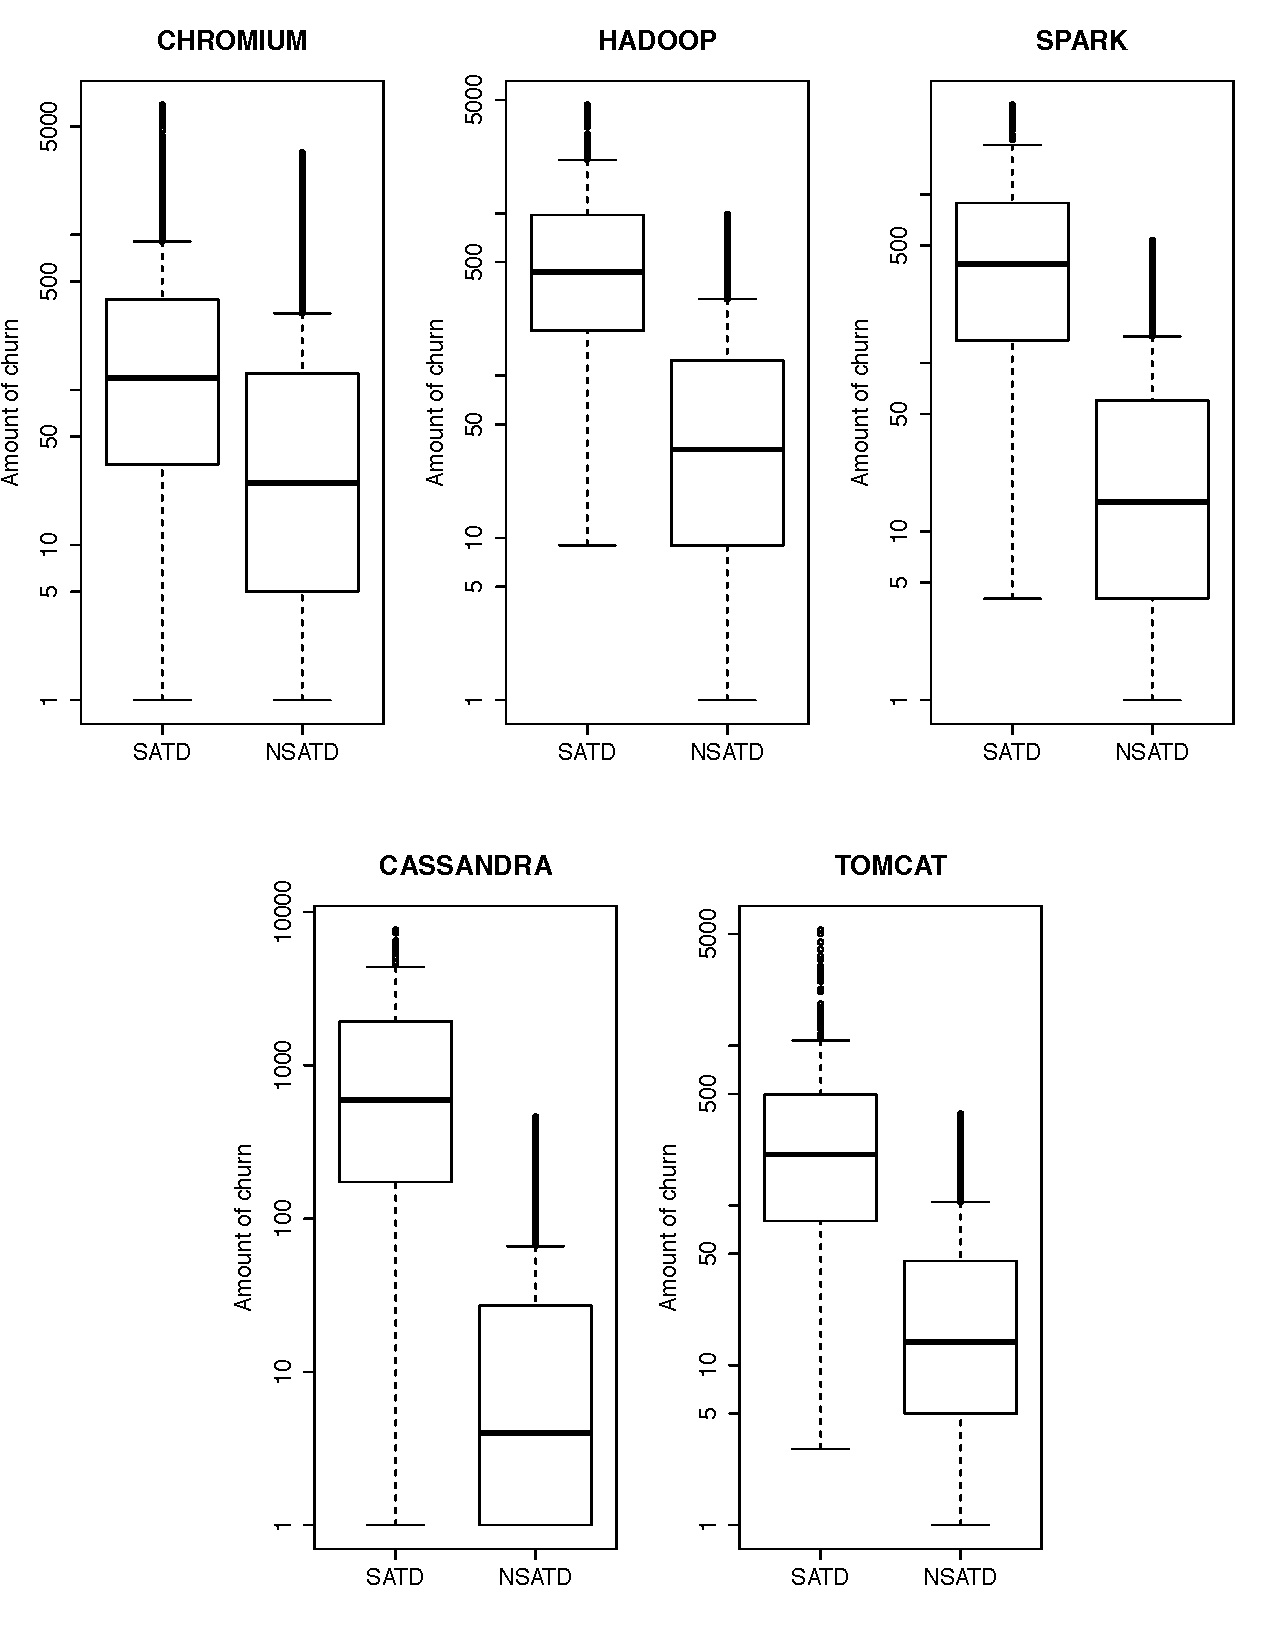
\includegraphics[width=90mm]{figures/chapter3/churn_for_all_projects}
	\caption{Total number of lines modified per change (SATD vs. NSATD).}
	\label{figure:tlcpc}
\end{figure}




\begin{figure}[h]
	\centering
	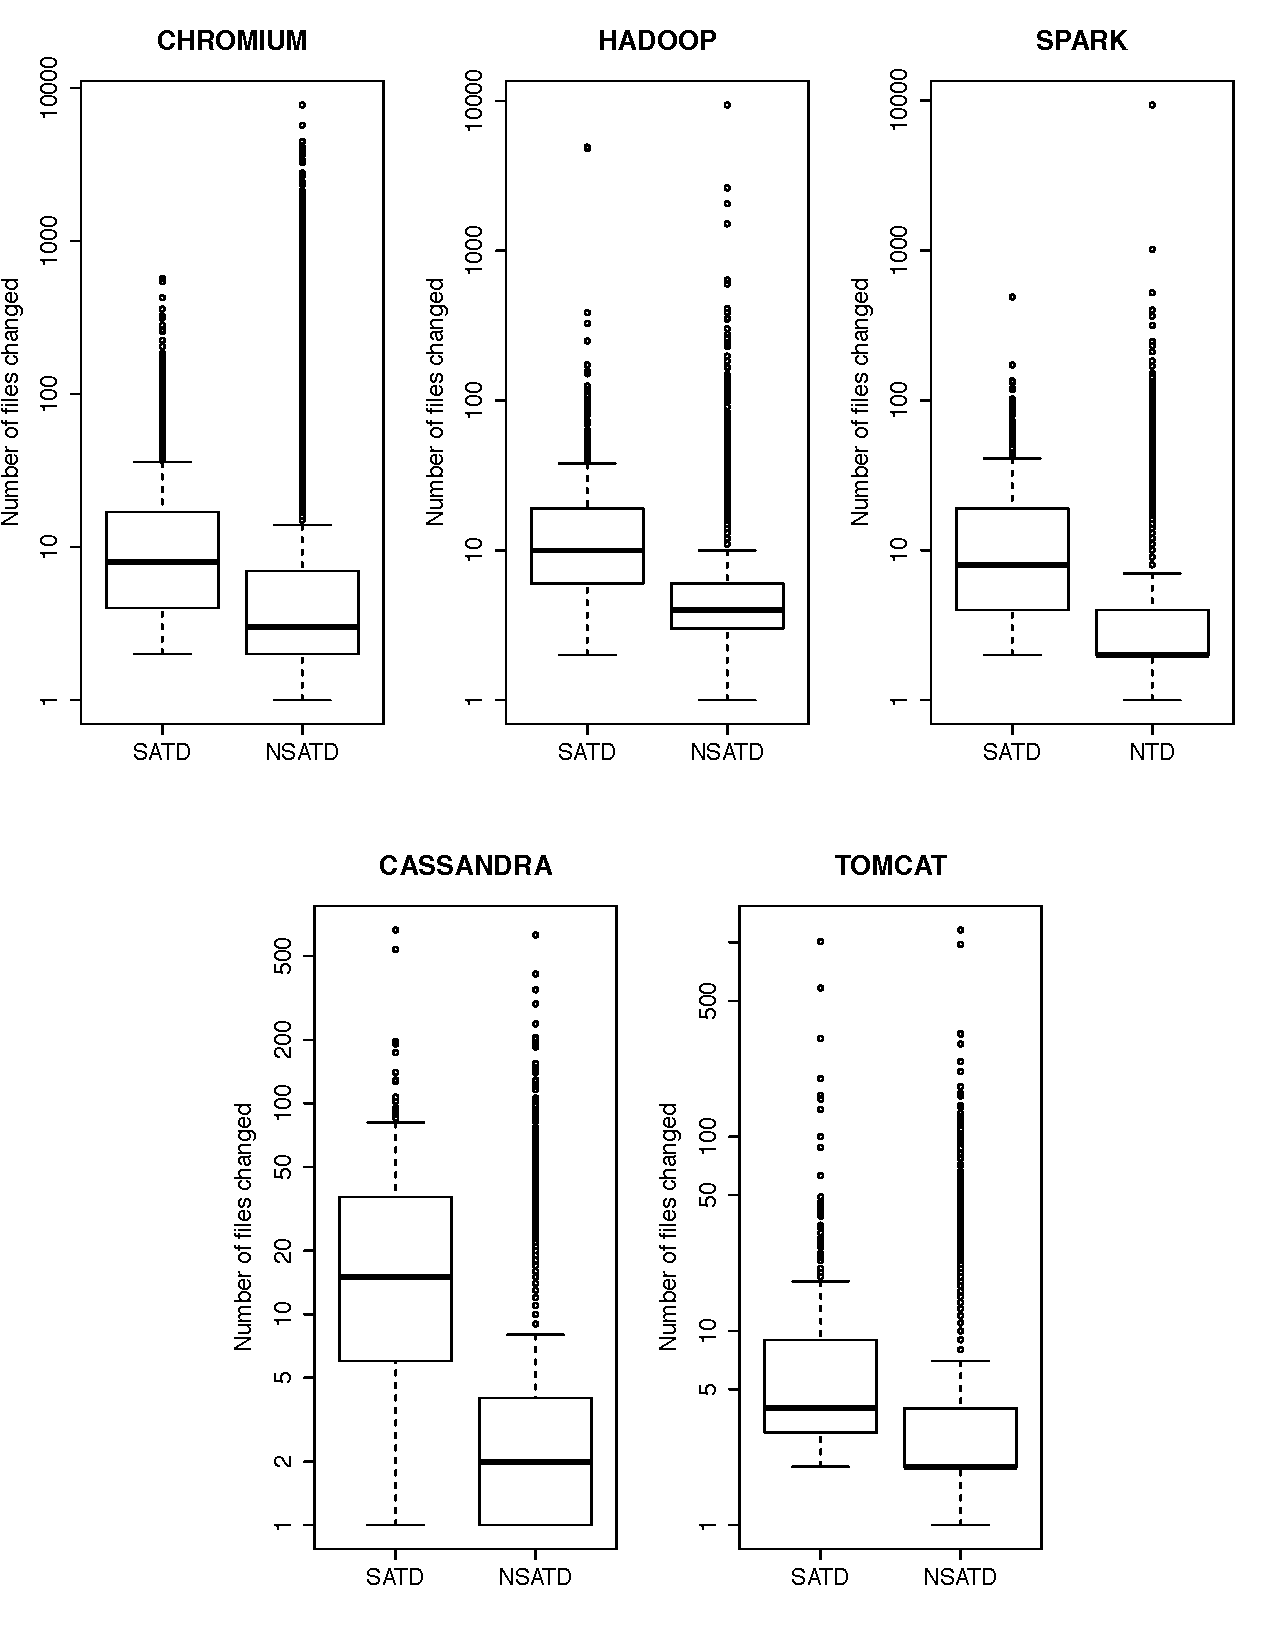
\includegraphics[width=90mm]{figures/chapter3/number_of_files_changed_all_projects}
	\caption{Total number of files modified per change (SATD vs. NSATD).}
	\label{figure:tfcpc}
\end{figure}

\begin{figure}[h]
	\centering
	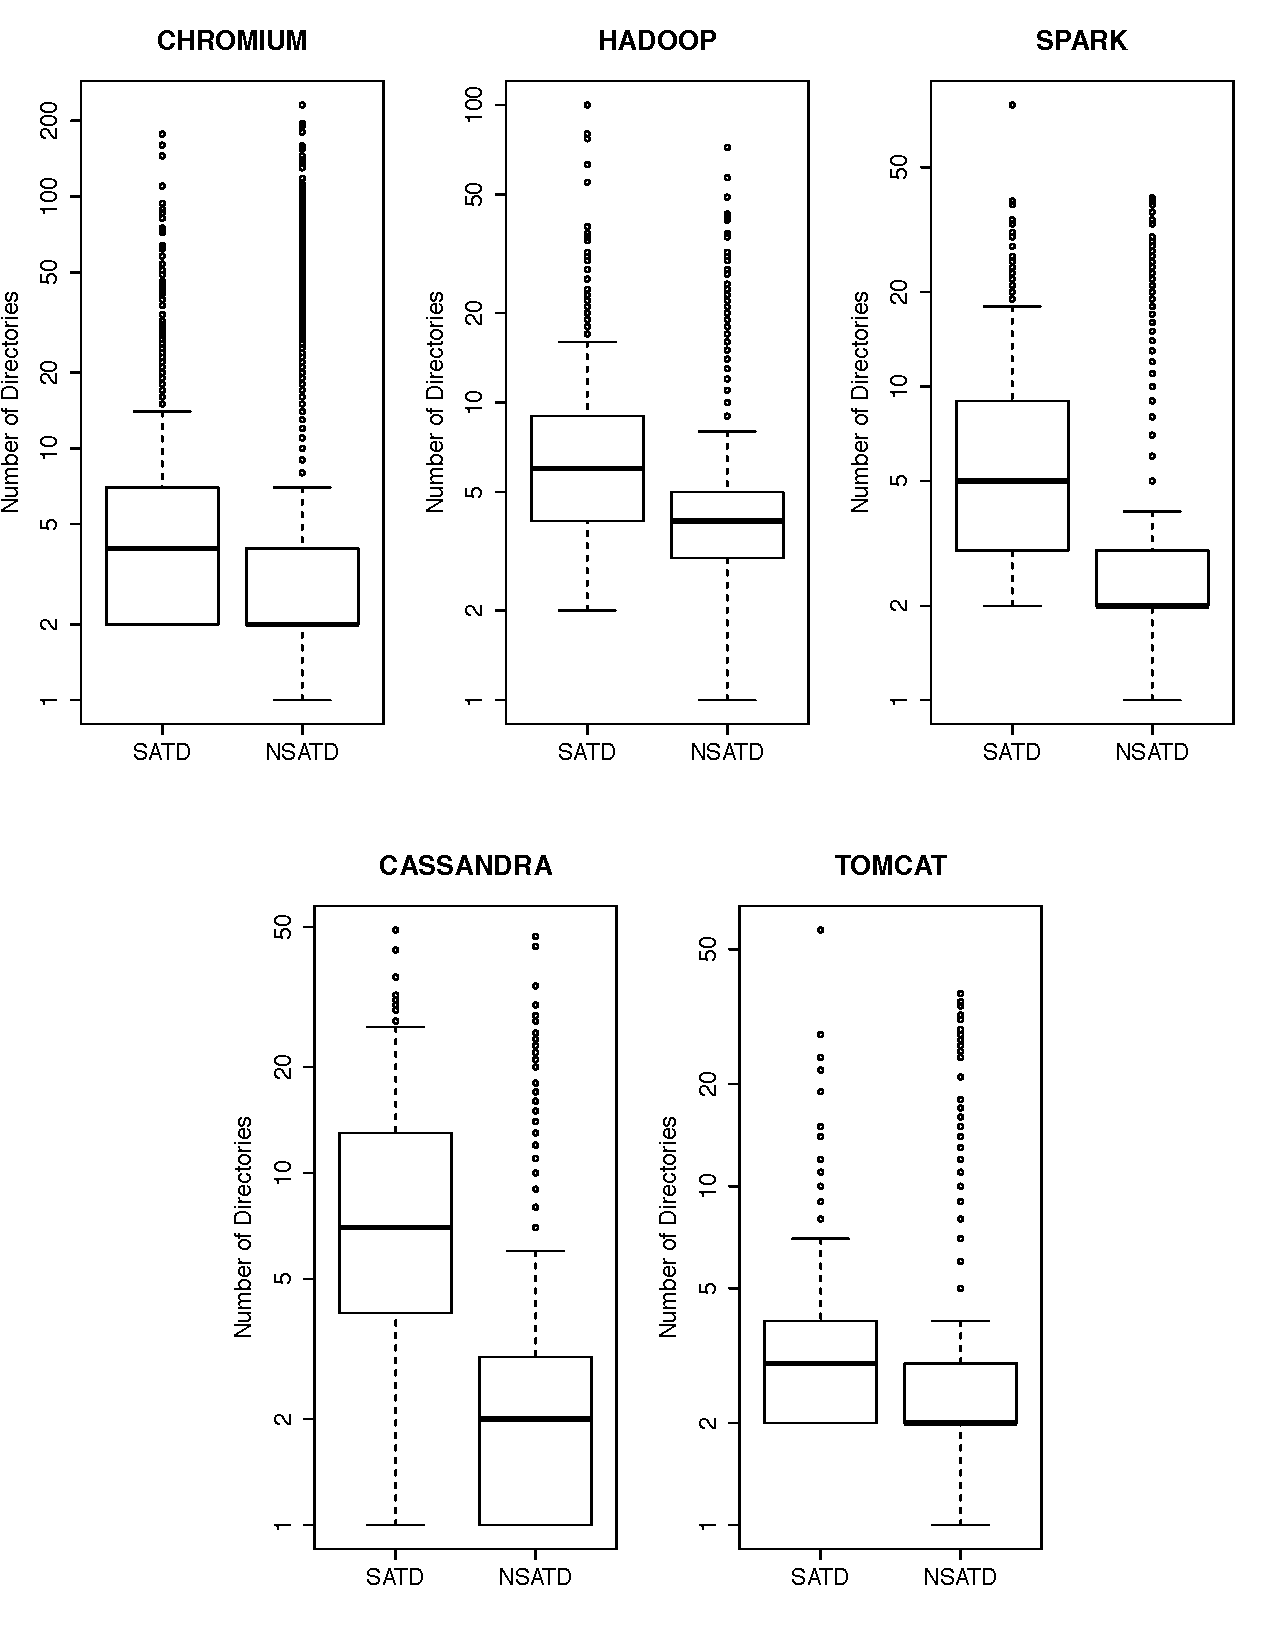
\includegraphics[width=90mm]{figures/chapter3/number_of_directories}
	\caption{Total number of modified directories per SATD and NSATD change.}
	\label{figure:number_of_directories}
\end{figure}


\begin{figure}[h]
	\centering
	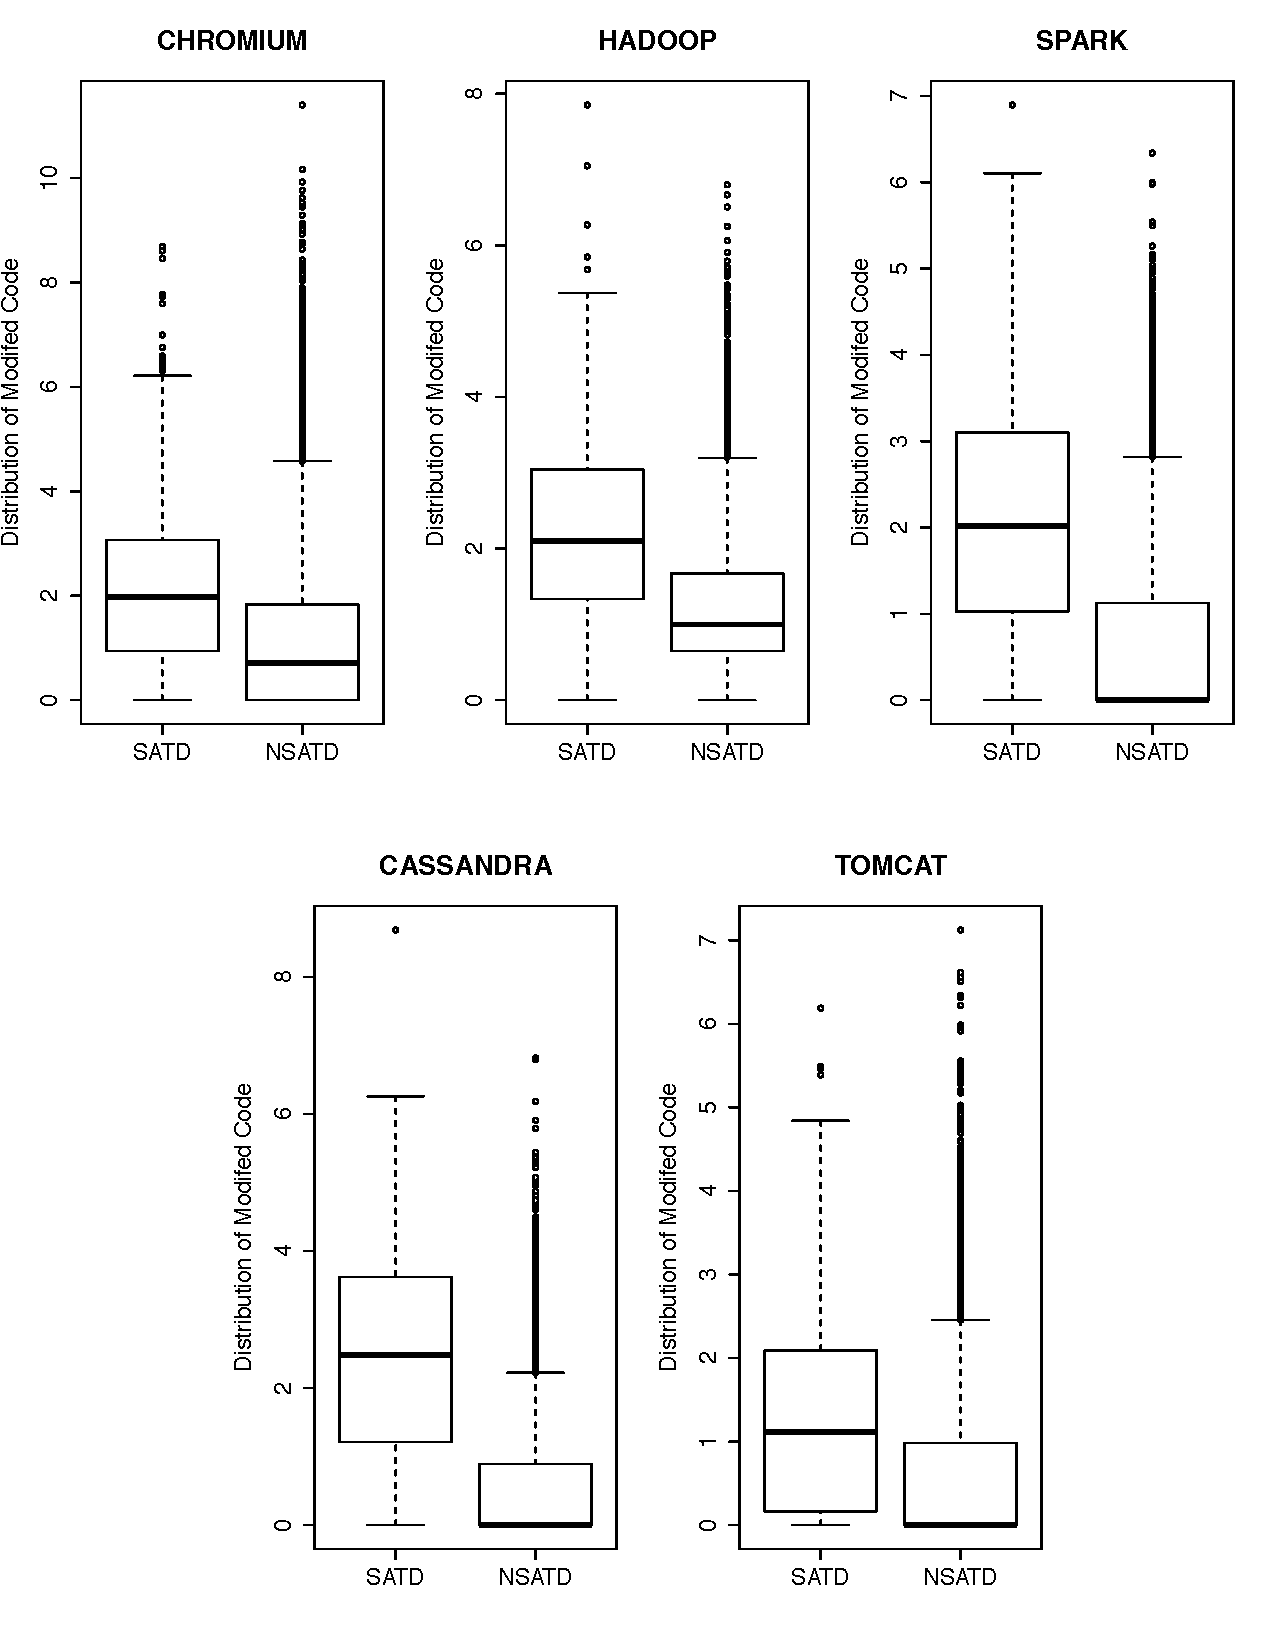
\includegraphics[width=90mm]{figures/chapter3/entropy_for_all_projects}
	\caption{Distribution of the change across the SATD and NSATD files.}
	\label{figure:mtdocatdf}
\end{figure}


To measure the entropy of a change, we use the change complexity measure proposed by Hassan~\cite{hassan2009predicting}. Entropy is defined as: $H(P)=-\sum _{k=1}^{n}\textrm ({p}_{k}*{log}_{2} {p}_{k})$, where $k$ is the proportion file$_{k}$ is modified in a change and $n$ is the number of files in the change. Entropy measures the distribution of a change across different files. Let us consider a change that involves the modification of three different files named \textit{A, B} and \textit{C} and let us suppose that the number of modified lines in files\textit{ A, B} and \textit{C} is 30, 20 and 10 lines, respectively. The entropy is equal to:
$(1.46=-\frac{30}{60}\log_{2}\frac{30}{60}-\frac{20}{60}\log_{2}\frac{20}{60}-\frac{10}{60}\log_{2}\frac{10}{60})$.

As in Hassan \cite{hassan2009predicting}, the above entropy formula has been normalized by the maximum entropy $log_{2}n$ to account for differences in the number of files per change. The higher the normalized entropy, the more difficult the change.




\noindent{\textbf{Results:}} Figures~\ref{figure:tlcpc},~\ref{figure:tfcpc},~\ref{figure:number_of_directories},~\ref{figure:mtdocatdf} reveal that for all difficulty measures, SATD changes have a higher value than non-SATD changes. We also find that the difference between the SATD and non-SATD changes is statistically significant, with a \textit{p}-value such that $p < 0.05$. Table~\ref{table:cliff_deltas_RQ3} shows the Cliff's delta effect size values for all projects studied. We observe that for all projects and all measures of difficulty, the effect size is either medium or large (Cf. Table~\ref{table:cliff_deltas_RQ3}), which indicates that SATD changes are more difficult than non-SATD changes.

In summary, we conclude that SATD changes are more difficult than non-SATD changes, provided that difficulty is measured using churn, the number of modified files, the number of modified directories and change entropy.







\section{Threats to Validity}
\label{chap3:sec:threats_to_validity}

Threats  to {\bf  internal validity}  concern any factors that could have confounded our study results. To identify \SATD, we use source code comments. In some cases, though, developers may not add comments when they introduce technical debt. The opposite poses another threat, namely, that developers might introduce technical debt and subsequently remove it without removing the related comment. In both cases the code and comment change inconsistently. However, Potdar and Shihab~\cite{ICSM_PotdarS14} examined this phenomenon in Eclipse and found that in 97\% of cases code and comments change in tandem. As a means of locating SATD, we use the comments compiled by Potdar and Shihab~\cite{ICSM_PotdarS14}, yet there is a possibility that these patterns do not detect all SATD. Additionally, given that comments are written in natural language, Potdar and Shihab had to manually read and analyze them to determine those that would indicate SATD. Manual analysis is prone to subjectivity and errors and therefore we cannot guarantee that all considered patterns will be perceived as SATD indicators by other developers. To mitigate this threat, we manually examined each comment that we detected and verified that it contained one of the 62 patterns in \cite{ICSM_PotdarS14}. We performed this step, independently, for each of the five projects studied. We identify a change as an SATD change if it contains at least one SATD file. Alternatively, we could have defined SATD changes as only those for which all files have SATD. We elected to do it the former way because sometimes SATD in just one file can impact the rest of the change, e.g. it may cause many other files to be changed. When measuring the percentage of file defects after the introduction of SATD, it is difficult to distinguish the differences due to SATD from those attributed to natural evaluation of the files.



Threats  to {\bf external validity} concern the possibility that our results may not generalize. To optimize generalizability, we analyzed five large open-source systems and drew our data from the well-established, mature codebase of open-source software projects with well-commented source code. These projects belong to different domains and they are written in different programming languages.


Furthermore, we focused on SATD only, which means that we do not cover all technical debt---there could well be other technical debt that is not self-admitted. Studying all technical debt is beyond the scope of this thesis.





\section{Conclusion and Future Work}
\label{chap3:sec:conclusion}



Technical debt is intuitively recognized as bad practice by software companies and organizations. However, there is very little empirical evidence on the extent to which technical debt can impact software quality. Therefore, in this thesis we perform an empirical study, using five large open-source projects, to determine precisely how technical debt relates to software quality. We focus on self-admitted technical debt, which refers to  errors that might be introduced as part of intentional and temporary quick fixes. As in  \cite{ICSM_PotdarS14}, we leverage source code comments to identify such debt on the basis of recurring indicator patterns.


We examined the relationship between self-admitted technical debt and software quality by investigating: (i) whether files with SATD have more defects compared to files without SATD, (ii) whether SATD changes introduce future defects and (iii) whether SATD-related changes tend to be more difficult. We measured the difficulty of a change in terms of amount of churn, number of files and modified modules and change entropy.




Our findings suggest that there is no reliable trend when it comes to defects and self-admitted technical debt. In some of the projects, self-admitted technical debt files had more bug-fixing changes, while in others, files without it had more defects. We also found that SATD changes are less correlated with future defects than non-SATD changes, but more difficult to perform. 
%\sultan{Our study demonstrates that although defects are not among the negative effects of technical debt, it can make the system more difficult to change in the future.}
Our study demonstrates that although technical debt may have negative effects, its impact does not extend to defects, but rather to making the system more difficult to change in the future.

We enlist empirical evidence in showcasing some of the drawbacks of technical debt that plague the software development process, in particular increases in system complexity. As a takeaway, practitioners would do well to keep technical debt in check and avoid its unwanted consequences. In the future, we intend to expound upon this research by studying the nature of defective SATD files more closely.


\chapter{Comparing the Impact of Comment- Versus Metric-Based Technical Debt}
\label{chapter4}
% -*- root: cuthesis_masters.tex -*-
\section{Introduction}
\label{chap4:sec:introduction}
\setlength\parindent{24pt} 

In the previous chapter, we studied the relationship between \SATD and software quality and found that the presence of SATD complicates future changes. Supplementing these comment-based indicators with the metric-based indicators used in earlier work \cite{zazworka2011investigating} (God Classes), we replicate the study conducted in chapter 3 on a larger scale in order to compare the relationship between both comment- and metric-based technical debt and quality. Of the foregoing studies that have covered how metric-based technical debt affects software quality, few have done so on large datasets. We remedy this on the one hand by integrating both comment- and metric-based approaches, as mentioned, and on the other by introducing a more granular analysis on the file and change levels. Empirically examining how both approaches relate to software quality and comparing any differences between them will provide researchers and practitioners with a more global understanding of technical debt, warn them of its future risks and raise awareness of the challenges it can pose.

Predictably, as technical debt has become a more popular strategy at developers' disposal, numerous advances have been made in detecting it, some metric-based and others comment-based. The former includes Marinescu's \cite{marinescu2004detection} methodology, which detects \textit{God Class} code smells according to sets of rules and thresholds defined on various object-oriented metrics. The latter, advocated by Potdar and Shihab's \cite{ICSM_PotdarS14} methodology in recent work, flags recurring source code comment patterns that correlate with incidence of \textit{self-admitted technical debt} (SATD). Moreover, the nature of the comments that developers leave has allowed occurrences of SATD to be sub-categorized and analyzed accordingly.

Without access to research that treats technical debt from all angles, developers will be misinformed as to the costs and benefits of technical debt and unequipped to decide responsibly whether it should be assumed in a given scenario---not to mention lacking effective strategies for keeping it in check once assumed. Our work closes this gap as we study 40 open-source projects that bring into focus the empirical links between both \SATD and god classes and software quality. If our results are true for a larger number of projects, then they are even more likely to generalize to others. 

Our inquiry pursues: (i) whether god class and SATD files have more defects than files free of god classes and SATD, (ii) whether god- and SATD-related changes introduce future defects, (iii) whether god- and SATD-related changes are associated with greater difficulty and (iv) to what extent the comment- and metric-based approaches identify the same instances of technical debt. As in the previous chapter, amount of churn, quantity of affected files and modified modules and change entropy all factor into the change difficulty calculations. In the end we observed that: (i) no straightforward correlation exists between incidence of SATD or god files and incidence of defects, (ii) more future defects surfaced after performing god and SATD changes than non-god and non-SATD changes and (iii) god and SATD changes are more difficult to perform than non-god and non-SATD changes. Preliminarily, (i)-(iii) concede that the downsides of god classes and \SATD are increases in future defect density and change difficulty. Yet the two approaches were found to reinforce each other in that (iv) between 11\% and 34\% of technical debt sources were identified by both the comment- and metric-based approaches.


%\section{Related Work}
%\label{chap4:sec:related_work}
%\todo{only mention the new studies, what have they found, talk about your study \& how it differs}
%Our work uses code comments and object-oriented metrics  to identify technical debt. Therefore, we divide the related work into four categories: source code comments, technical debt, software quality, and identifying and detecting code smells.
%\subsection{Source Code Comments}
%Developers have tapped into the many advantages of source code comments in prioritizing, delegating and finalizing personal and team tasks~\cite{Storey:2008}. Another benefit has to do with how comments contribute to a greater understanding of the programs with which they are affiliated~\cite{TakangGM96}; without them, pinpointing program defects quickly becomes a ``needle in a haystack" kind of scenario. In order to avoid such situations, developers must monitor code-comment consistency, ensuring that changes in the code are updated in the comments and vice versa, and to this end, Tan \textit{et al.} recommend @iComment for detecting lock- and call-related inconsistencies~\cite{tan07icomment}, @aComment for interrupt context synchronization inconsistencies~\cite{acomment} and @tComment for inconsistencies emanating from exceptions to inferred Javadoc properties~\cite{tcomment}. Even so, code-comment inconsistencies are not as prevalent as one might expect, Fluri \textit{et al.}~\cite{fluri2007code} having determined the rate of co-changed code and comments to be 97\%.

%Malik \textit{et al.}~\cite{malik2008understanding} identify the rate of changed call dependencies and control statements, modified function age and the amount of co-changed dependent functions as the foremost attributes leading to source code comment updates. Given the importance of keeping comments consistent with high-level artifacts and stabilizing source code identifiers, De Lucia \textit{et al.}~\cite{DeLucia2011} conducted a study that verified---through a series of controlled experiments---that a resemblance between source code and high-level software artifacts does improve comment and identifier quality.

%Source code comments are also salient in the arena of \SATD detection, as Potdar and Shihab~\cite{ICSM_PotdarS14} demonstrated in researching to what extent and for what reasons SATD is introduced and how often it is subsequently removed. In fact, comments served as the basis of Maldonado and Shihab's~\cite{MTD15p9} SATD classification system and allowed them to quantify the incidence of the five types they identified. At a rate of 42\% to 84\% of 33,000 classified comments, design debt was easily the most common.

%\subsection{Technical Debt}

%Several major studies have centered on technical debt besides SATD---technical debt that source code analysis tools are deployed to detect. Zazworka \textit{et al.}~\cite{Zazworka:2013}, weighing the merits of automated and manual detection strategies, concur that the returns on engineering more tools and heuristics capable of detecting technical debt would greatly advance the field as it now stands. Looking at how god classes influence maintainability later in the development process, Zazworka \textit{et al.}~\cite{zazworka2011investigating} established that god classes are changed more frequently and harbor more defects than their non-god counterparts and thus that the undesirable ramifications of technical debt might extend to software quality. Guo \textit{et al.}~\cite{GuoSGCTSSS11} monitored the lifecycle of one delayed task and specified how some of the consequences of technical debt surface in real time.

%\subsection{Software Quality}
%Studies in the same vein as~\cite{Zimmerman2008Springer} have been devoted to outlining the factors that either do detract or could detract from software quality and raising awareness among project contributors. However, metrics, too, have been used to isolate defects, including: design and code~\cite{Jiang-promise-2008}, code churn~\cite{Nagappan-icse-2005} and process metrics~\cite{Moser-icse-2008,Rahman-icse-2013}.

%The likes of the SZZ algorithm originated by Sliwerski \textit{et al.}~\cite{Sliwerski-fse-2005} and Kim \textit{et al.}'s~\cite{Kim-tse-2008} defect-proneness identifiers excerpted from change logs and added or deleted source code mark a shift in defect prediction towards the change level. The former links a version archive to a bug database in order to isolate fix-inducing changes~\cite{Sliwerski-fse-2005}, whereas Kamei's~\cite{Kamei-tse-2013} ``Just-In-Time Quality Assurance" approach exemplifies how process metrics outdo product metrics in identifying risky software changes.

%\subsection{Identifying and Detecting Code Smells}
%Fowler and Beck \cite{fowler1999refactoring} originated the term \textit{code smell} to designate various indicators of object-oriented design flaws which can undermine software maintenance. Code smells respond to the internal and external properties of the system elements they monitor. Though manual code smell detection warns developers of potential vulnerabilities, Marinescu \cite{Marinescu_ICETOOLS} observes that it is time-consuming, non-repeatable and non-scalable. Apart from this, the more familiar the software system is to a developer, the higher the risk of a subjective appraisal of its efficiencies and shortcomings, according to Mäntylä \cite{mantyla2003taxonomy, mantyla2004bad}, and one important corollary of this is that a developer's chances of overlooking design flaws increase. In order to surmount these drawbacks, Marinescu recommends enlisting code metrics to detect system volatilities, and in this spirit, several implementations of this departure from manual detection have been devised \cite{lanza2007object, marinescu2004detection, Marinescu_PhD, Marinescu_IBM_JRD}.

\section{Approach}
\label{chap4:sec:approach}
As we continue to study the interplay between \SATD and metric-based debt (God Classes) and software quality, measures must be established in order to quantify software quality \cite{Kamei-tse-2013,Kim-tse-2008,sliwerski-msr-2005}. The precedent in accomplishing this task has been to count the defects in SATD files and calculate the rate of future defect introduction among SATD changes, expressed as a percentage. Deferring to the technical debt metaphor and its concept of accruing ``interest" to be paid in the long run, we also measure software quality in terms of SATD change difficulty, which we calculate as stipulated earlier. With these metrics standardized, we entertain the research questions that follow:

\begin{itemize}
	\vspace{0.1cm}
	\item {\bf RQ1:} Do god and SATD files have more defects than non-god and non-SATD files?
	%\vspace{0.1cm}
	\item {\bf RQ2:} Do god- and SATD-related changes introduce future defects?
	%\vspace{0.2cm}
	\item {\bf RQ3:} Are god- and SATD-related changes more difficult than non-god and non-SATD changes?
	%\vspace{0.2cm}
	\item {\bf RQ4:} Is there an overlap between comment- and metric-based technical debt? 
\end{itemize}

We devised a suitable methodology, visualized in Figure \ref{fig:CH4_Process_overview}, to guide our inquiry into these questions. We initiate the process by mining the source code repositories and pulling source code files on a project-by-project basis (steps 1-2). Afterwards the source code files are parsed and comments extracted (step 3). We then identify all instances of \SATD, count defects file-wide and isolate defect-inducing changes by means of the SZZ algorithm (steps 4-5).

\begin{figure}[h]
	\centering
	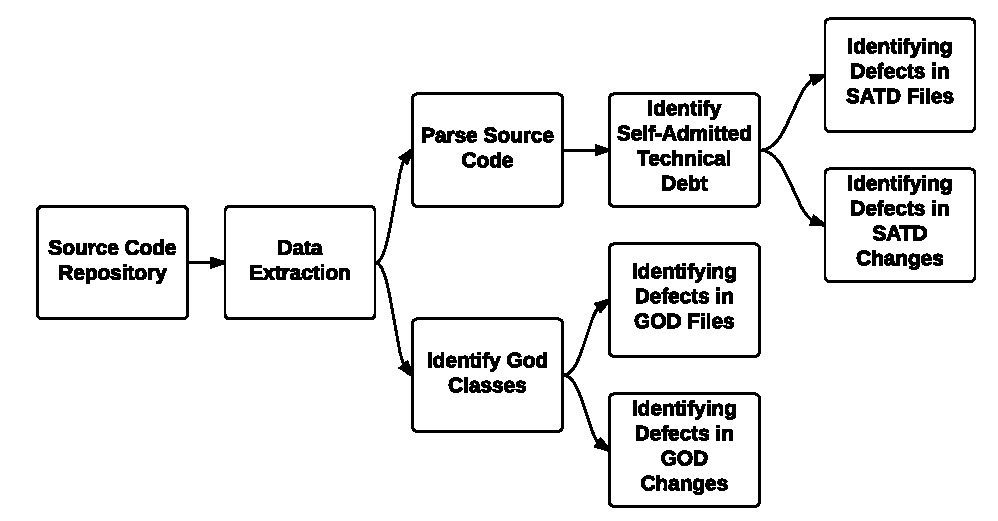
\includegraphics[width=150mm]{figures/chapter4/approach}
	\caption{Metric-based (God Classes) approach overview.}
	\label{fig:CH4_Process_overview}
\end{figure}


\subsection{Data Extraction}

To generalize the scope of this study, we relied on certain criteria in selecting the 40 open-source software projects: (i) well-commented source code, (ii) varying numbers of lines of code (LOC), (iii) different numbers of contributors, (iv) different development domains, (v) mature development history and (vi) issue tracking system capability. The first criterion is a prerequisite for Potdar and Shihab's SATD detection technique; the last is essential to accurately study the introduction of future defects.

Given the extent to which our approach to locating \SATD relies on source code comments, we downloaded the most recent versions of the relevant systems, filtered this input to generate source code and excluded all files lacking source code comments (\eg{} CSS, XML, JSON). As for comments suspected of indicating no SATD, e.g. license comments, commented source code, Javadoc comments, etc., four filtering heuristics were deployed to remove them from the results.

Tables \ref{table:ch4_projects_statistics} and \ref{table:ch4_projects_statistics_2} showcase some key identifiers and statistics for each project, including: (i) which release was downloaded, (ii) the number of lines of code it contains, (iii) the number of comment lines, (iv) a source code file count, (v) the number of committers in the project's development history and (vi) its commit count.

\begin{landscape}


\begin{table}[htbp]
	\small
	\centering
	\caption{Characteristics of the studied projects (part 1).}
	\begin{adjustbox}{width=1.3\textwidth}


		\begin{tabular}{l|l|c|c|c|c|c}
			\hline
			\textbf{Project}           & \textbf{Release} & \textbf{\# Lines of Code} & \textbf{\# Comment Lines} & \textbf{\# Files} & \textbf{\# Committers} & \textbf{\# Commits} \\ \hline
			\textbf{Apache OpenNLP}    & 1.7.1            &          163,114           &           30,581           &        861        &           11           &        1,339         \\ \hline
			\textbf{Apache Camel}      & 2.18.0           &          1,626,040          &          430,818           &       17,046       &          333           &        25,461        \\ \hline
			\textbf{Apache Habse}      & ‎1.2.4           &          1,310,985          &          251,409           &       3,243        &          166           &        12,531        \\ \hline
			\textbf{Apache Groovy}     & 2.4.2            &          286,920           &           85,885           &       1,517        &          262           &        13,422        \\ \hline
			\textbf{Apache Oltu}       & 1.0.2            &           267,88           &           7,386            &        300        &           14            &         842         \\ \hline
			\textbf{Apache Maven}      & 3.3.9            &          150,724           &           34,830           &       1,540        &           81           &        10,370        \\ \hline
			\textbf{Apache Karaf}      & 5.4.0            &          155,675           &           32,906           &       1,467        &           86           &        5,666         \\ \hline
			\textbf{Apache Hama}       & 0.6.4            &           855,64           &           22,545           &        499        &           22           &        1,592         \\ \hline
			\textbf{Apache Tomee}      & 1.7.4            &          854,611           &          212,542           &       6,297        &           35           &        10,257        \\ \hline
			\textbf{Apache Deltaspike} & 1.7.2            &          149,871           &           45,722           &       1,842        &           48           &        2,044         \\ \hline
			\textbf{Apache Curator}    & 2.10.0           &          124,077           &           18,458           &        525        &           66           &        1,813         \\ \hline
			\textbf{Apache Calcite}    & 1.10.0           &          448,820           &          110,410           &       1,702        &          102           &        2,180         \\ \hline
			\textbf{Apache Poi}        & 3.15             &          644,284           &          182,823           &       3,298        &           39           &        7,963         \\ \hline
			\textbf{Apache Zeppelin}   & 0.6.2            &          124,865           &           15,314           &        552        &          201           &        2,642         \\ \hline
			\textbf{Apache Ant}        & 1.9.7            &          343,010           &          109,150           &       1,927        &           62           &        13,425        \\ \hline
			\textbf{Apache Stanbol}    & 1.0.0            &          339,699           &          107,208           &       2,044        &           25           &        3,398         \\ \hline
			\textbf{Apache Kafka}      & 0.10.1           &          152,685           &           33,368           &       1,002        &          300           &        2,734         \\ \hline
			\textbf{Apache Tika}       & 1.13             &          142,786           &           38,984           &        992        &           54           &        3,209         \\ \hline
			\textbf{Apache Felix}      & ‎5.4.0           &          837,955           &          211,404           &       5,039        &           51           &        13,240        \\ \hline
			\textbf{Apache Phoenix}    & 4.9.0            &          396,054           &           69,326           &       1,620        &           59           &        1,748         \\ \hline
		\end{tabular}
		\label{table:ch4_projects_statistics}

\end{adjustbox}

\end{table}

\end{landscape}



\begin{landscape}

	
	
	\begin{table}[htbp]
		\small
		\centering
		\caption{Characteristics of the studied projects (part 2).}
		\begin{adjustbox}{width=1.3\textwidth}
			
			
			\begin{tabular}{l|l|c|c|c|c|c}
				\hline
				\textbf{Project}           & \textbf{Release} & \textbf{\# Lines of Code} & \textbf{\# Comment Lines} & \textbf{\# Files} & \textbf{\# Committers} & \textbf{\# Commits} \\ \hline
				\textbf{Apache Wicket}     & 7.5.9            & 548,923                    &          191,279           &       4,830        &           80           &        19,574        \\ \hline
				\textbf{Apache Aurora}     & 0.16.0           & 317,551                    &           70,774           &       1,284        &          105           &        3,639         \\ \hline
				\textbf{Apache Ignite}     & 1.6              & 1,498,260                   &          443,157           &       7,361        &          117           &        17,933        \\ \hline
				\textbf{Apache Helix}      & 0.7.1            & 141,632                    &           34,430           &        900        &           32           &        2,266         \\ \hline
				\textbf{Apache Archiva}    & 2.2.1            & 191,743                    &           33,641           &       1,172        &           41           &        7,742         \\ \hline
				\textbf{Apache Struts}     & 2.5              & 316,495                    &           83,911           &       2,307        &           65           &        4,634         \\ \hline
				\textbf{Apache Derby}      & 10.13.1.1        & 1,271,629                   &          386,703           &       3,023        &           37           &        8,127         \\ \hline
				\textbf{Apache Ambari}     & ‎2.4.2           & 2,220,418                   &          421,937           &       10,223       &          119           &        18,025        \\ \hline
				\textbf{Apache Nifi}       & 1.0.0            & 576,512                    &          118,806           &       3,493        &          120           &        2,826         \\ \hline
				\textbf{Apache Tiles}      & 3.0.7            & 51,487                     &           20,173           &        599        &           16           &        1,455         \\ \hline
				\textbf{Apache Shiro}      & ‎1.3.2           & 81,131                     &           36,854           &        727        &           22           &        1,641         \\ \hline
				\textbf{Apache Usergrid}   & 2.1.0            & 605,286                    &          114,999           &       2,619        &          110           &        10,621        \\ \hline
				\textbf{Apache Nutch}      & 2.3              & 104,214                    &           27,478           &        843        &           37           &        2,217         \\ \hline
				\textbf{Apache Zookeeper}  & 3.4.9            & 196,008                    &           38,867           &        814        &           21           &        1,468         \\ \hline
				\textbf{Apache Mina}       & 2.0.16           & 45,588                     &           14,336           &        340        &           29           &        2,400         \\ \hline
				\textbf{Apache Cxf}        & 3.1.8            & 988,585                    &          196,520           &       8,806        &           81           &        12,302        \\ \hline
				\textbf{Apache CloudStack} & 4.9.0            & 1,423,346                   &          207,036           &       6,424        &          412           &        29,931        \\ \hline
				\textbf{Apache Oozie}      & 4.3.0RC0         & 256,423                    &           49,510           &       1,239        &           22           &        1,772         \\ \hline
				\textbf{Apache Kylin}      & 1.5.4.1          & 217,645                    &           45,320           &       1,227        &           89           &        5,121         \\ \hline
				\textbf{Apache Flink}      & 1.1.2            & 791,670                    &          195,738           &       4,154        &          325           &        9,513         \\ \hline
			\end{tabular}
			\label{table:ch4_projects_statistics_2}
			
		\end{adjustbox}
		
	\end{table}
	
\end{landscape}


\subsection{Scanning Code and Extracting Comments}

Now source code comments must be extracted from the projects under investigation, for which we implement a Python-based tool. The rest of the extraction process is the same as for subsection \ref{ch3_scanningCodeAndExtracting}. 

%Having isolated the source code from all of the projects under investigation, we implemented a Python-based tool to extract the source code comments. Beyond this, the tool reveals each comment's type (i.e., single-line or block comments), the name of its host file and its line number. The Count Lines of Code (CLOC) tool ~\cite{cloc} double checks the Python-based tool, and provided that there is no discrepancy between the total number of lines of comments both yield, we have confidence in the accuracy of the tool we developed.

\subsection{Filter Comments}


Source code comments left by developers might situate the project within the circumstances of its development, communicate their recommendations for revising the code at a later date, acknowledge who wrote which pieces or who made which fixes or confess that self-admitted technical debt has been assumed. Efforts should be made to decrease the volume of comments, especially when sifting through them in search of \SATD confessions. For this reason, we make use of several filtering heuristics proposed by Moldonado \textit{et al.} \cite{Maldonado_TSE2017} to focus our search query.\par

A Python-based tool reads data retrieved from parsed source code, initiates the filtering heuristics and stores the results in the database. The retrieved data specify each class or comment's starting and ending line numbers as well as Java syntax comment type (i.e., single-line, block or Javadoc). Once this information is acquired, the filtering heuristics are processed. \par

Self-admitted technical debt is seldom indicated in comments left prior to class declaration, e.g. license comments, among others, so we benefit from any mechanism that identifies and omits such distractors without also omitting comments that incorporate Java IDE task annotations (i.e., ``TODO:", ``FIXME:" or ``XXX:"). If a comment features any of these keywords, tasks related to the comment will be added to an IDE-generated list for ease of access. As for separating pre- and post-class declaration comments, the number of the line in which the class is declared marks the crucial cutoff in that any preceding comments are targeted for removal.\par

Comment type matters insofar as cumbersome comments stitched together from single-line comment components (and not block comments) impede message interpretation for comments read one by one. A heuristic that pinpoints and collapses sequences of adjacent single-line comments into block comments overcomes the comment type issue.\par



Commented source code does not indicate \SATD in our experience, but rather either code not used at all or code used exclusively for debugging. To eliminate this distractor, we use a regular expression to remove typical Java code structures, i.e., public, private, for, exception, etc.\par


Most IDEs auto-generate comments when creating a method, constructor, try catch, etc. Due to the nature of the auto-generation of these comments, there is no SATD content. The majority of Javadoc comments also fail to mention SATD, and those that do are annotated with at least one task (i.e., ``TODO:", ``FIXME:", ``XXX:"). This criterion allows our heuristic to determine which Javadoc comments should be salvaged versus ignored, while no distinction is necessary for auto-generated comments. We designed a regular expression to apply the criterion by checking for task annotations before omitting the comment.\par




The procedure was conceived with the intention of factoring out the contribution of noise, which ultimately improves the quality of the comment dataset by reducing cases of SATD false positives and prioritizing the most applicable comments.\par



\subsection{Identifying Self-Admitted Technical Debt}
\label{ch4_td}


Our analysis hinges on locating \SATD at two levels: (i) the file level and (ii) the change level.

\noindent\textbf{SATD files:}
We emulated Potdar and Shihab \cite{ICSM_PotdarS14} in identifying \SATD on the basis of 62 different patterns recurring in multiple projects at various frequencies. The specifics of these patterns can be found in subsection \ref{ch3_td}.


\noindent\textbf{SATD changes:}
At the change level, all the files touched by the same change are checked for evidence of \SATD. If any one of them is determined to be an SATD file, the whole change is classified as an SATD change. Alternatively, if none of the files touched by a change is an SATD file, the whole change falls into the non-SATD change category. In general, the more SATD files a system contains, the more likely it is to have a higher number of SATD changes. SATD comments are shown to account for less than 6.10\% and SATD files for somewhere between 1.37\% and 25.03\% of the respective totals for all systems in Tables~\ref{table:projects_satd_god_percentage} and \ref{table:projects_satd_god_percentage2}, where each system's percentages are listed separately for comparison.

\begin{landscape}
	
	
	\begin{table}[htbp]
		\small
		\centering
		\caption{Percentage of SATD and God of the analyzed projects (part 1).}
		\begin{adjustbox}{width=1.0\textwidth}
			
			
			\begin{tabular}{l|c|c|c}
				\hline
				\textbf{Project}  & \textbf{SATD Comments (\%)}  & \textbf{SATD Files (\%)} & \textbf{God Files (\%)} \\ \hline
				\textbf{Apache OpenNLP} &  2.66 & 19.02 & 14.77   \\ \hline
				\textbf{Apache Camel} &  0.95 & 3.53 & 12.95    \\ \hline
				\textbf{Apache Habse} & 1.69 &  18.29 & 15.05    \\ \hline
				\textbf{Apache Groovy} &  3.41 & 13.67 & 14.52    \\ \hline
				\textbf{Apache Oltu} &  1.91 & 5.67 & 14.27    \\ \hline
				\textbf{Apache Maven} &  3.76 & 10.65 & 13.92    \\ \hline
				\textbf{Apache Karaf} &  2.40 & 7.44 & 14.58   \\ \hline
				\textbf{Apache Hama} &  1.44 & 11.24 & 14.48    \\ \hline
				\textbf{Apache Tomee} &  1.94 & 7.16 & 14.33   \\ \hline
				\textbf{Apache Deltaspike} &  3.95 & 9.28 & 9.26    \\ \hline
				\textbf{Apache Curator} &  0.99 & 5.34 & 15.32    \\ \hline
				\textbf{Apache Calcite} &  1.67 & 12.97 & 14.54    \\ \hline
				\textbf{Apache Poi} &  2.11 & 16.79 & 14.43    \\ \hline
				\textbf{Apache Zeppelin} &  1.62 & 9.37 & 14.87    \\ \hline
				\textbf{Apache Ant} &  2.23 & 20.56 & 14.60   \\ \hline
				\textbf{Apache Stanbol} &  4.03 & 25.03 & 14.06   \\ \hline
				\textbf{Apache Kafka} &  1.56 & 7.73 & 11.71    \\ \hline
				\textbf{Apache Tika} &  3.29 & 19.28 & 14.40    \\ \hline
				\textbf{Apache Felix} & 1.88 & 9.72 & 13.59   \\ \hline
				\textbf{Apache Phoenix} &  3.34 & 13.81 & 13.47    \\ \hline
				
			\end{tabular}
			\label{table:projects_satd_god_percentage}
			
		\end{adjustbox}
		
	\end{table}
	
\end{landscape}



\begin{landscape}
	
	
	
	\begin{table}[htbp]
		\small
		\centering
		\caption{Percentage of SATD and God of the analyzed projects  (part 2).}
		\begin{adjustbox}{width=1.0\textwidth}
			
			
			\begin{tabular}{l|c|c|c}
				\hline
				\textbf{Project}  & \textbf{SATD Comments (\%)}  & \textbf{SATD Files (\%)} & \textbf{God Files (\%)} \\ \hline
				\textbf{Apache Wicket} &  0.89 & 5.29 & 11.52    \\ \hline
				\textbf{Apache Aurora} &  3.97 & 14.27 & 14.91    \\ \hline
				\textbf{Apache Ignite} &  0.26 & 3.12 & 13.50   \\ \hline
				\textbf{Apache Helix} &  4.02 & 18.09 & 15.62    \\ \hline
				\textbf{Apache Archiva} &  6.05 & 17.71 & 12.61    \\ \hline
				\textbf{Apache Struts} &  1.85 & 8.07 & 12.39    \\ \hline
				\textbf{Apache Derby} &  1.20 & 22.66 & 14.37    \\ \hline
				\textbf{Apache Ambari} &  2.29 & 8.76 & 13.31   \\ \hline
				\textbf{Apache Nifi} &  0.87 & 4.62 & 13.29    \\ \hline
				\textbf{Apache Tiles} &  0.17 & 1.37 & 10.90    \\ \hline
				\textbf{Apache Shiro} &  2.67 & 15.86 & 12.85    \\ \hline
				\textbf{Apache Usergrid} &  2.20 & 11.20 & 12.33    \\ \hline
				\textbf{Apache Nutch} &  2.17 & 12.25 & 15.60    \\ \hline
				\textbf{Apache Zookeeper} &  1.71 & 10.31 & 13.82   \\ \hline
				\textbf{Apache Mina} &  1.12 & 5.99 & 14.71   \\ \hline
				\textbf{Apache Cxf} &  2.78 & 6.87 & 14.04   \\ \hline
				\textbf{Apache CloudStack} &  1.98 & 10.42 & 14.04   \\ \hline
				\textbf{Apache Oozie} &  1.63 & 9.73 & 15.81   \\ \hline
				\textbf{Apache Kylin} &  1.64 & 8.06 & 15.38   \\ \hline
				\textbf{Apache Flink} &  0.57 & 3.72 & 14.84   \\ \hline
				
			\end{tabular}
			\label{table:projects_satd_god_percentage2}
			
		\end{adjustbox}
		
	\end{table}
	
\end{landscape}


\subsection{God Classes}
God classes are classes that combine trivial class workloads and generally avoid assigning tasks to other classes. They are distinguishable on account of their high complexity, low inner-class cohesion and frequent foreign class data access \cite{lanza2007object}. Object-oriented design advocates a one-to-one correspondence between classes and responsibilities, which god classes violate by definition \cite{lanza2007object}. Due to their size and the extent to which they are tied to other classes, god classes can make it more difficult to understand the system \cite{fowler1999refactoring} and are expected to be more susceptible to defects during system maintenance. The higher the incidence of defects, the more often changes will have to be performed and the bigger those changes will be, compounding maintenance over time \cite{fowler1999refactoring, lanza2007object}.

\subsection{Identifying God Classes}
\label{ch4_god}

To perform our analysis, we need to identify god classes at the same two levels as \SATD: (i) the file level and (ii) the change level.

\noindent\textbf{God files:} To identify god classes, we followed the methodology outlined by Marinescu \cite{marinescu2004detection}, who proposed an approach to specify and detect
code smells, specifically \textit{God Classes}. Their technique leverages metric-based heuristics that identify god classes according to sets of rules and thresholds defined on various object-oriented metrics. The formula provided below in Figure \ref{equation:1} operates on three metrics---namely, weighted method count (WMC), tight class cohesion (TCC) and access to foreign data (ATFD)---and generates one of two outputs. If the output is 1, then the class to which the formula is applied is a god class; if 0, it is a non-god class.

\noindent\textbf{God changes:}
To study the relationship between god classes and quality at the change level, we must first identify which classes are god classes and which are non-god classes. By analogy with the technique used to identify SATD and non-SATD changes, we consider any change containing at least one god file to be a god change and those containing no god files to be non-god changes. 


\begin{figure}[h]
\[GodClass(C) = \left\{\begin{matrix}
1& (AFTD(C), HigherThan(1))  \wedge ((WMC(C), TopValues(25\%)) \vee \\ 
 & (TCC, BottomValues(25\%)))\\ 
0& else
\end{matrix}\right.\]
\captionsetup[figure]{list=no}
\caption{God Class Detection Equation}
\label{equation:1}
\end{figure}

The equation in Figure~\ref{equation:1} above describes how we detect a god class, where:


\begin{itemize}
\item[$\bullet$] \textbf{Weighted Method Count (WMC)} is the sum of the statistical complexity of all methods in a class \cite{Chidamber_Kemerer_94}. McCabe's cyclomatic complexity \cite{McCabe_1976} is used as a complexity measure for all class methods.
\item[$\bullet$] \textbf{Tight Class Cohesion (TCC)} is the number of directly connected public methods in a class \cite{Bieman:1995:CRO:223427.211856}.
\item[$\bullet$] \textbf{Access to Foreign Data (ATFD)} is the number of external classes whose attributes are accessed either directly or indirectly (by accessor methods) \cite{Marinescu_PhD}.
\end{itemize}

\subsection{Identifying Defects in God Files and God Changes}
\label{ch4_bugs_td}

According to Sliwersky \textit{et al.} \cite{sliwerski-msr-2005}, expressions denoting defect identifiers, e.g. ``\textit{fixed issue, bug ID, fix, defect, patch, crash, freeze, breaks, wrong, glitch, properly, proper}," ordinarily certify that an earlier mistake has been corrected when recorded in control system change logs. Other work has proposed comparable methodologies for tracking fault-inducing changes until repaired \cite{Kamei-tse-2013, Kim-tse-2008, sliwerski-msr-2005}. Next we pull each defect report from its corresponding issue tracking system, i.e., Bugzilla~\footnote{https://www.bugzilla.org} or JIRA~\footnote{https://www.atlassian.com/software/jira}, and comb for all pertinent details. Once the god files and god changes have been separated, we go about determining the number of file defects and identifying any defect-inducing changes in the same way foregoing research has ~\cite{Kamei-tse-2013, Kim-tse-2008, sliwerski-msr-2005}.

\noindent\textbf{Defects in files:}
A file defect count is a prerequisite to any defectiveness comparison between god and non-god files. With this in mind, we first view a file's history and extract all the changes that have touched it. The list this produces is then shortened as change log searches return only results consistent with keywords indicating corrective changes.
Examples of these keywords can be found in subsection \ref{ch3_bugs}, along with the steps we take to rule out false positives.


\noindent \textbf{Defect-inducing changes:}
Along the same lines, we search the commit messages using regular expressions that convey defect fixes as a means of establishing whether a given change is corrective. The keywords used to identify corrective changes are given in subsection \ref{ch3_bugs}, where the procedure for identifying defect-inducing changes is presented.

\section{Case Study Results}
\label{chap4:sec:case_study_results}

In this section, we present the empirical outcomes of our inquiry into the correlation between both self-admitted technical debt and god classes and software quality. Each of the three research questions is restated below, where we summarize its motivation, our approach in treating it and the conclusions we reached. Statistics and results are listed for all individual projects, accompanied by cross-project comparisons.

%\sultan{stopped here}
\subsection*{\chapterIVrqI}


\noindent{\textbf{Motivation:}}
Reluctance to resort to code smells and technical debt suggests that most developers believe these adversely affect software quality, and what research has been conducted supports this conviction~\cite{zazworka2011investigating}. %\sultan{I'm not sure how to incorporate god classes in this case since there has been a lot of work that studied their impact on software quality}
The potential drawbacks of SATD, meanwhile, have remained unexplored despite its research-affirmed ubiquity in software projects \cite{ICSM_PotdarS14}. Researchers and developers should be better equipped to negotiate the long-term risks of SATD and have empirical evidence in hand that identifies concrete issues its use can bring about, raising SATD literacy within the community at large.


\noindent{\textbf{Approach:}}
We compare god files versus non-god files and SATD files versus non-SATD files in terms of defect-proneness.


\noindent\textbf{Comparing god and non-god files:}
The God Class Detection Equation proposed by \cite{marinescu2004detection} provides a way to identify god classes using object-oriented metrics. Files are fed to the equation and are labeled either god or non-god files, depending on the output. We calculate the normalized value of defect-fixing changes for each file in both categories based on $\frac{ \#~of~fixing~changes}{SLOC}$. We normalize our data by dividing the number of defect-fixing changes by the number of source lines of code, since god files are inherently large, and apply a test designed to measure whether the differences between the categories are statistically significant.

In case this distribution is non-normal, we use the non-parametric Mann-Whitney~\cite{mann1947test} test because, unlike the parametric alternatives, it is capable of handling such distributions. A \textit{p}-value such that $p \le 0.05$ indicates that the difference between the samples is statistically significant.


\noindent\textbf{Comparing SATD and non-SATD files:}
We identify SATD files in accordance with the procedure detailed in section~\ref{ch3_td}, labeling files containing any number of SATD comments as SATD files and all others non-SATD files. These two file categories (SATD and non-SATD) undergo calculations yielding the percentage of defect-fixing changes, $\frac{ \#~of~fixing~changes}{SLOC}$ , which, unlike pure counts, standardizes the metric across files hosting different numbers of source lines of code. Afterwards the defect distribution is plotted for SATD and non-SATD files and a test is performed to uncover any statistical trends.

Again, we elected to conduct the non-parametric Mann-Whitney~\cite{mann1947test} test to decide whether a statistical difference exists between the SATD and non-SATD groups rather than a parametric substitute, which could not accommodate non-normal distribution. A statistically significant difference returns a \textit{p}-value of at most 0.05 ($p \le 0.05$).


\noindent{\textbf{Results - Defects in god files vs. non-god files and SATD files vs. non-SATD files:}}


\begin{figure}[h]
	\centering
	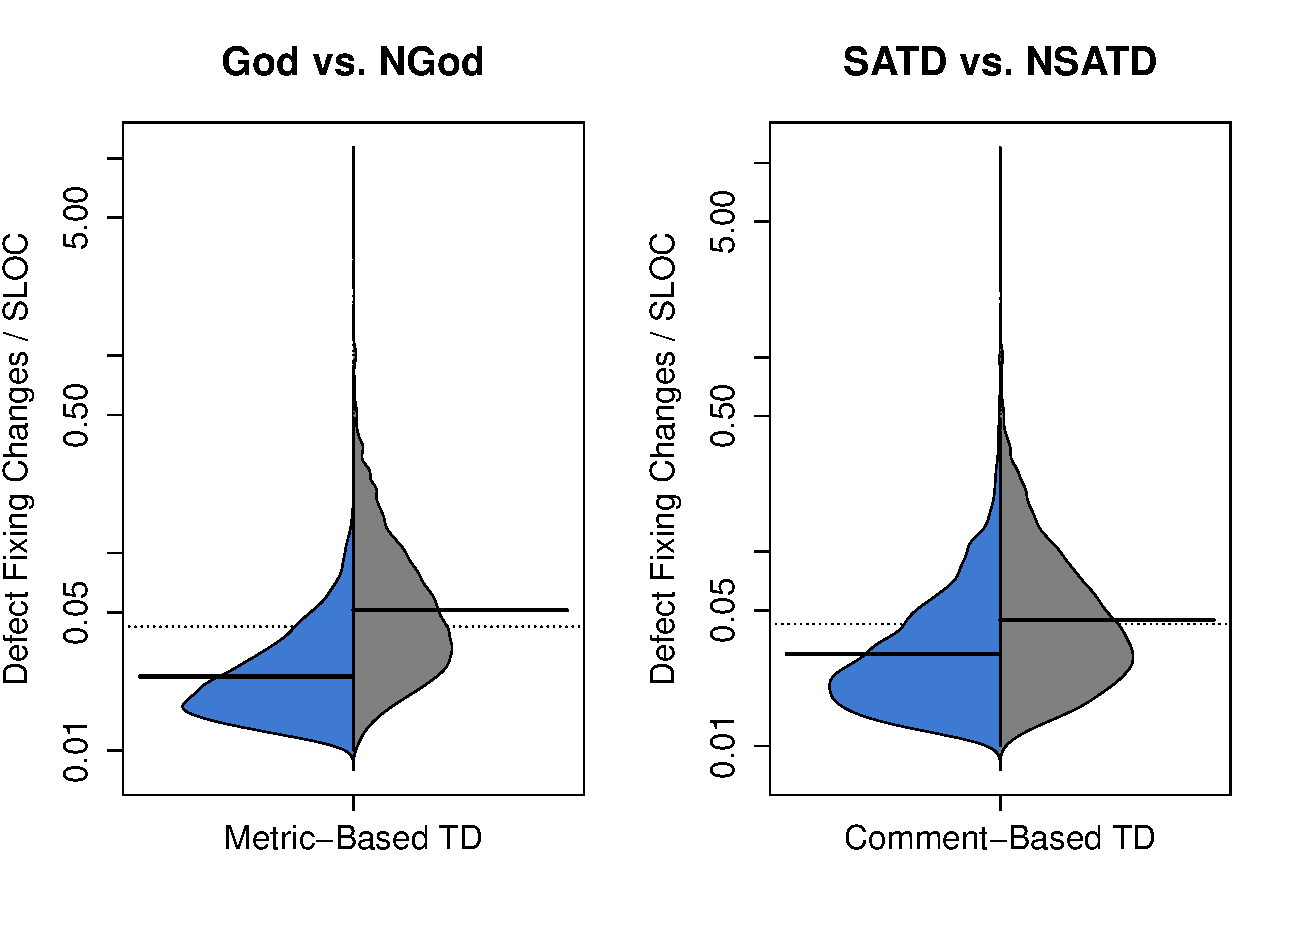
\includegraphics[width=140mm]{figures/chapter4/rq1_defectivness_distrubution_new2}
	\caption{Percentage of defect-fixing changes for (i) God vs. non-God files and (ii) SATD vs. NSATD files.}
	\label{figure:ch4_number_of_fixing_changes_TD_vs_NTD}
\end{figure}

Beanplots are a convenient way to present and compare univariate data for two groups. Those in Figure \ref{figure:ch4_number_of_fixing_changes_TD_vs_NTD} display the distribution of \textit{median corrective change rates}, based on $\frac{ \#~of~fixing~changes}{SLOC}$, for god files versus non-god files and SATD files versus non-SATD files \textit{in each project}. %These rates represent the number of bug-fixing changes over the number of total changes.
The dotted lines represent the overall mean taking data from both groups into account; for this reason, the dotted lines mark the same value on both sides of each beanplot. The solid lines, in contrast, mark the median value for each group and thus differ from one side to the other. A comparison of \textit{distribution medians} indicates that the defectiveness rates for god and SATD files are lower than the corresponding rates for non-god and non-SATD files.

\begin{myboxii}[RQ1 - Interim Summary]
	Neither god files nor \SATD files are associated with a higher percentage of defects.
\end{myboxii}

Figure~\ref{figure:percentage_of_defects_god_vs_ngod} (in the appendix) shows boxplots for the individual projects which compare the distribution of defectiveness rates for god and non-god files. We can see that the rate is higher for non-god files than god files within each project and that this difference is statistically significant such that $p \le 0.05$, which holds when all project medians are consolidated in the distribution in Figure \ref{figure:ch4_number_of_fixing_changes_TD_vs_NTD}.

Although Figure \ref{figure:ch4_number_of_fixing_changes_TD_vs_NTD} indicates that non-SATD files have a higher median defectiveness rate than SATD files, this trend is not borne out in every individual project. In Figure \ref{figure:percentage_of_defects_td_vs_ntd}, we observe that OpenNLP, Curator and Tiles constitute exceptions where the defectiveness rate is higher among SATD files.


\subsection*{\chapterIVrqII}


\noindent{\textbf{Motivation:}}
Having looked at how god and non-god and SATD and non-SATD compare at the file level, we turn our sights to the question of whether god and SATD changes introduce future defects at a higher rate than non-god and non-SATD changes. Before, entire files were the objects of our analysis; now we require an analysis tailored to assess individual changes.


To investigate how change category relates to introduction of future defects and the duration of the ``grace period" before software quality is affected, we should first determine to what extent god classes and SATD are predisposed to introduce future defects. Our conjecture is that god and SATD changes introduce future defects at a higher rate than non-god and non-SATD changes. Further, we expect that if a god or SATD change causes a defect to be introduced in the change right after, then the delay is minimal and the impact on quality cannot be put off for very long.


\noindent{\textbf{Approach:}}
We identify defect-inducing changes utilizing the SZZ algorithm~\cite{sliwerski-msr-2005} and subdivide the results it generates into four categories depending on whether the changes contain god classes or not (god versus non-god defect-inducing changes) and whether they contain SATD or not (SATD versus non-SATD defect-inducing changes). We then apply the Mann-Whitney test \cite{mann1947test} to evaluate the statistical significance of the difference between god versus non-god defect-inducing changes and SATD versus non-SATD defect-inducing changes (from the same respective data sets). If the resulting \textit{p}-value is such that $p \le 0.05$, then the difference is not attributable to chance but rather statistically significant, and generalizes to other data sets.


\noindent{\textbf{Results:} God and non-god distributions of defect-inducing change rates in each project share a common vertical axis in the first plot in Figure \ref{figure:ch4_bug_inducing_changes}, as do SATD and non-SATD defect-inducing change rate distributions in the second. We observe that the distribution median (i.e., the median of the individual project medians) is higher for the god and SATD changes than for the non-god and non-SATD changes. This indicates that god and SATD changes have more of a tendency to induce future defects than their non-god and non-SATD counterparts. We also find that the differences between god versus non-god and SATD versus non-SATD defect-inducing changes are both statistically significant with $p \le 0.05$.


\begin{myboxii}[RQ2 - Interim Summary]
	Both god changes and SATD changes tend to introduce a higher number of future defects.
\end{myboxii}

\begin{figure}[h]
	\centering
	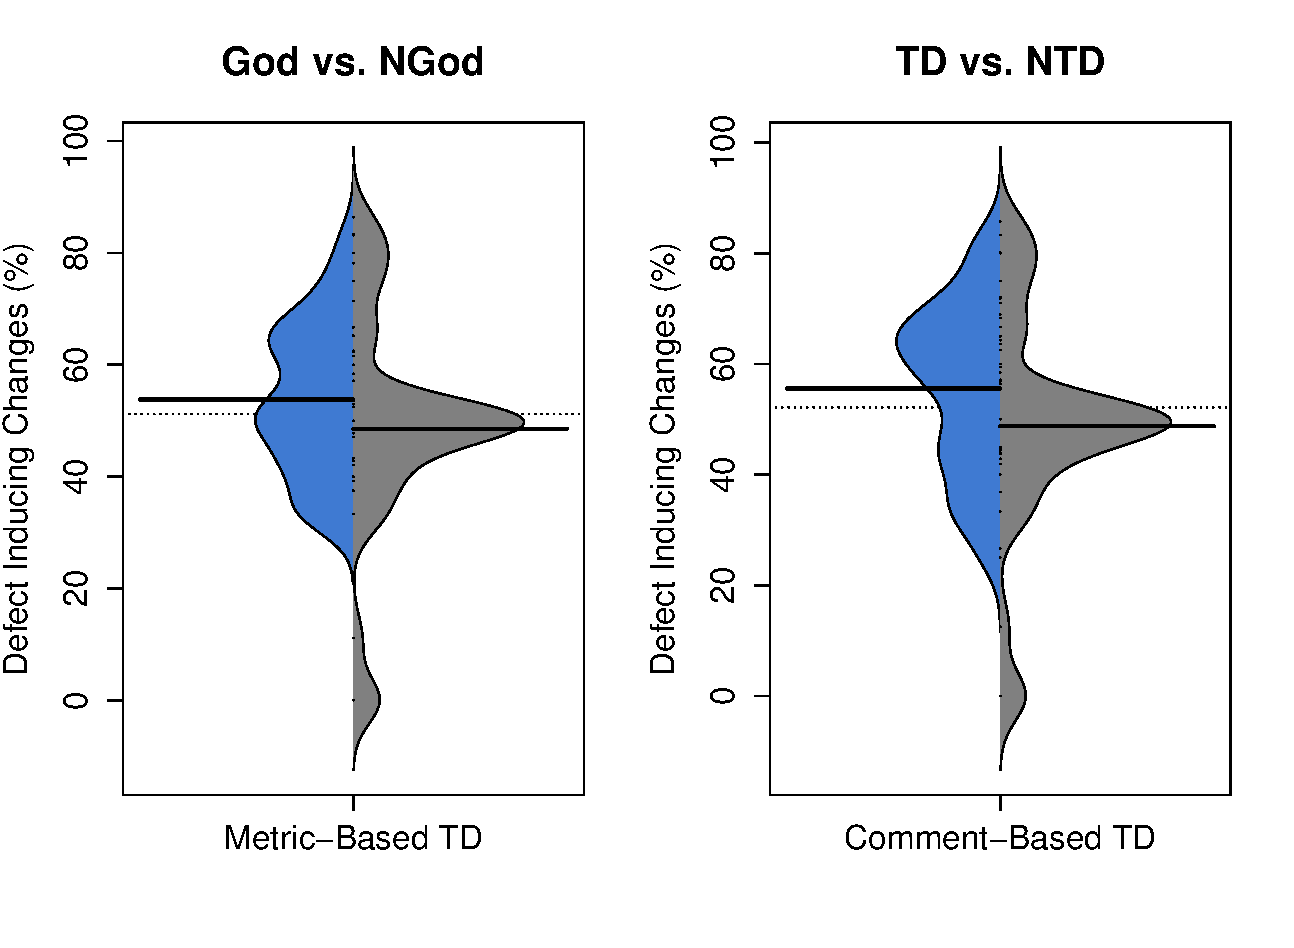
\includegraphics[width=140mm]{figures/chapter4/rq2_new}
	\caption{Percentage of defect-inducing changes for (i) God vs. non-God and (ii) SATD vs. NSATD.}
	\label{figure:ch4_bug_inducing_changes}
\end{figure}

As a general rule, what is true of the distribution medians is also true of individual project medians, though exceptions exist---among them Apache Hbase, Apache Kafka, Apache Mina, Apache Shiro, Apache Oozie, Apache Flink, Apache Deltaspike and Apache curator in Figures \ref{figure:percentage_of_bug_inducing_god_vs_ngod} and \ref{figure:percentage_of_bug_inducing_td_vs_ntd}. In these projects, the non-god and non-SATD changes appeared to induce more future defects than the god and SATD changes. These isolated counterexamples, while in conflict with the trend observed in Figure \ref{figure:ch4_bug_inducing_changes}, are compatible with our findings in chapter 3, where we report that SATD changes have less of a tendency to induce future defects.

\subsection*{\chapterIVrqIII}

\noindent{\textbf{Motivation:}}
Up to this point, we have been concentrating on the interplay between both god classes and SATD and defects lowering software quality. As we know from previous research \cite{marinescu2004detection}, god classes violate object-oriented design principles and have negative long-term implications for system maintainability. Likewise, if we recall the ramifications of the technical debt metaphor, we see that the short-term payoff should come at an increased cost later on in development. The deferred consequences of god classes and technical debt are measured in terms of increasing difficulty, which has yet to be fully examined after detecting god classes and introducing technical debt. Verifying that god classes and SATD do increase change difficulty will better portray their implications for future changes and software projects and in the end enable developers to see the full picture when deciding whether or not to refactor god classes or introduce \SATD. \\

\noindent{\textbf{Approach:}}
We recognize god, non-god, SATD and non-SATD change categories and compare the difficulty of executing changes from each category. We reuse the four metrics from chapter 3 to determine change difficulty: churn, the number of modified directories, the number of modified files and the entropy of the change. For a slightly different purpose, Eick \emph{et al.}~\cite{eick2001decay} chose the first three to measure decay; Hassan~\cite{hassan2009predicting} utilized the last metric to measure change complexity. As in RQ2, we use the Mann-Whitney test \cite{mann1947test} to determine whether the differences between god and non-god changes and between SATD and non-SATD changes are statistically significant and measure the effect size using Cliff's delta \cite{Cliff:2005}, this time with respect to the complexity metric categories. 


%To measure the change churn, number of files and number of directories, we extract these metrics from the change log. To calculate churn for a whole change, we add up the number of lines inserted and deleted in each individual file touched by the change. To count the files and directories touched by a change, we extract the list of files from the change log. We consider a directory to be \textbf{ND} and a file to be \textbf{NF} when measuring the number of modified directories and files. Thus, if a change involves the modification of a file having the path ``src/os/unix/ngx\_alloc.h," then the directory is \textit{src/os/unix} and the file is \textit{ngx\_alloc.h}.\\



\begin{figure}[!hp]
	\centering
	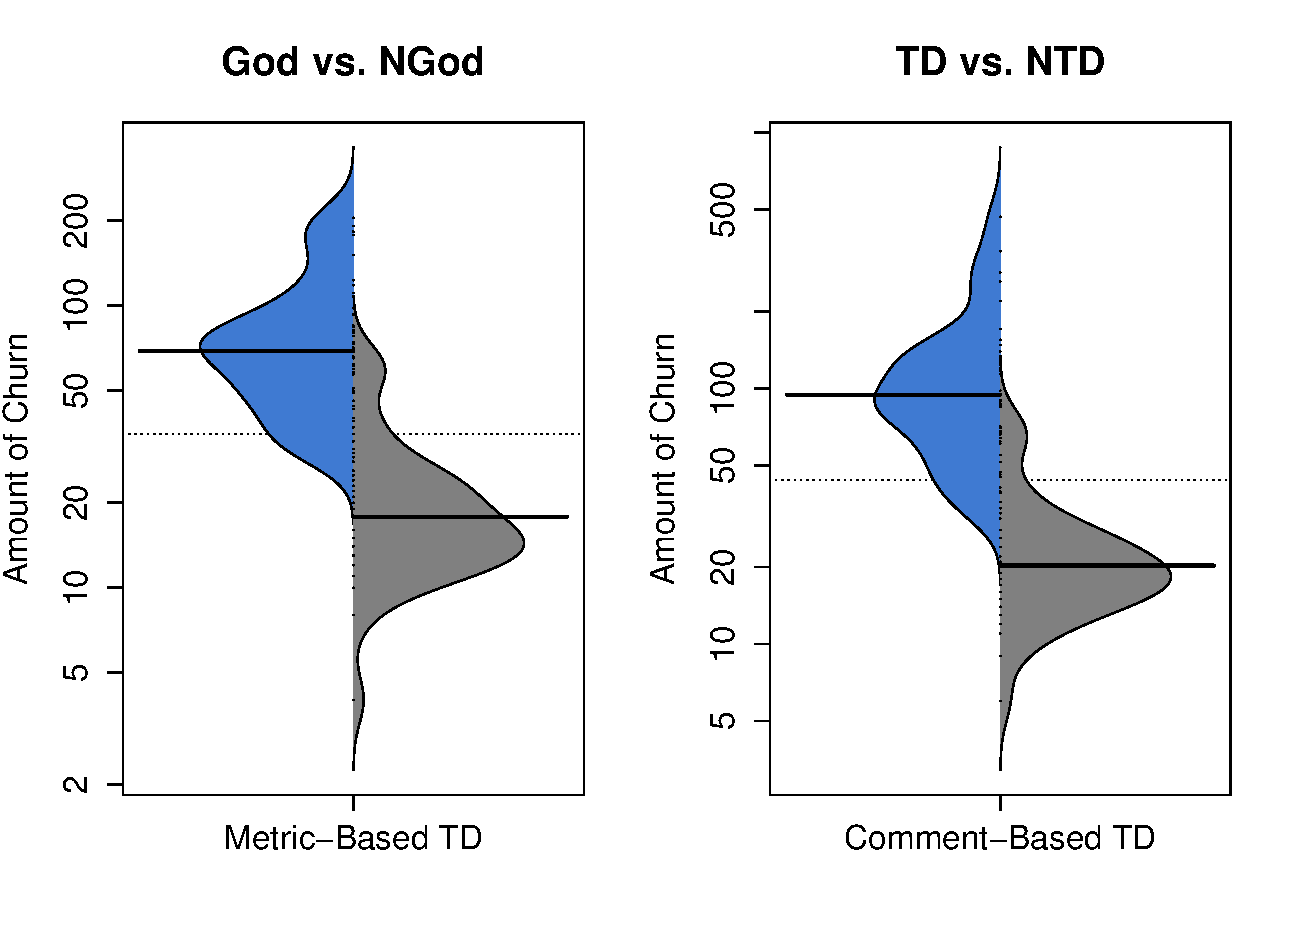
\includegraphics[width=120mm]{figures/chapter4/rq3_churn}
	\caption{Total number of lines modified per change for (i) God vs. non-God and (ii) SATD vs. NSATD.}
	\label{figure:ch4_tlcpc}
\end{figure}



\begin{figure}[!hp]
	\centering
	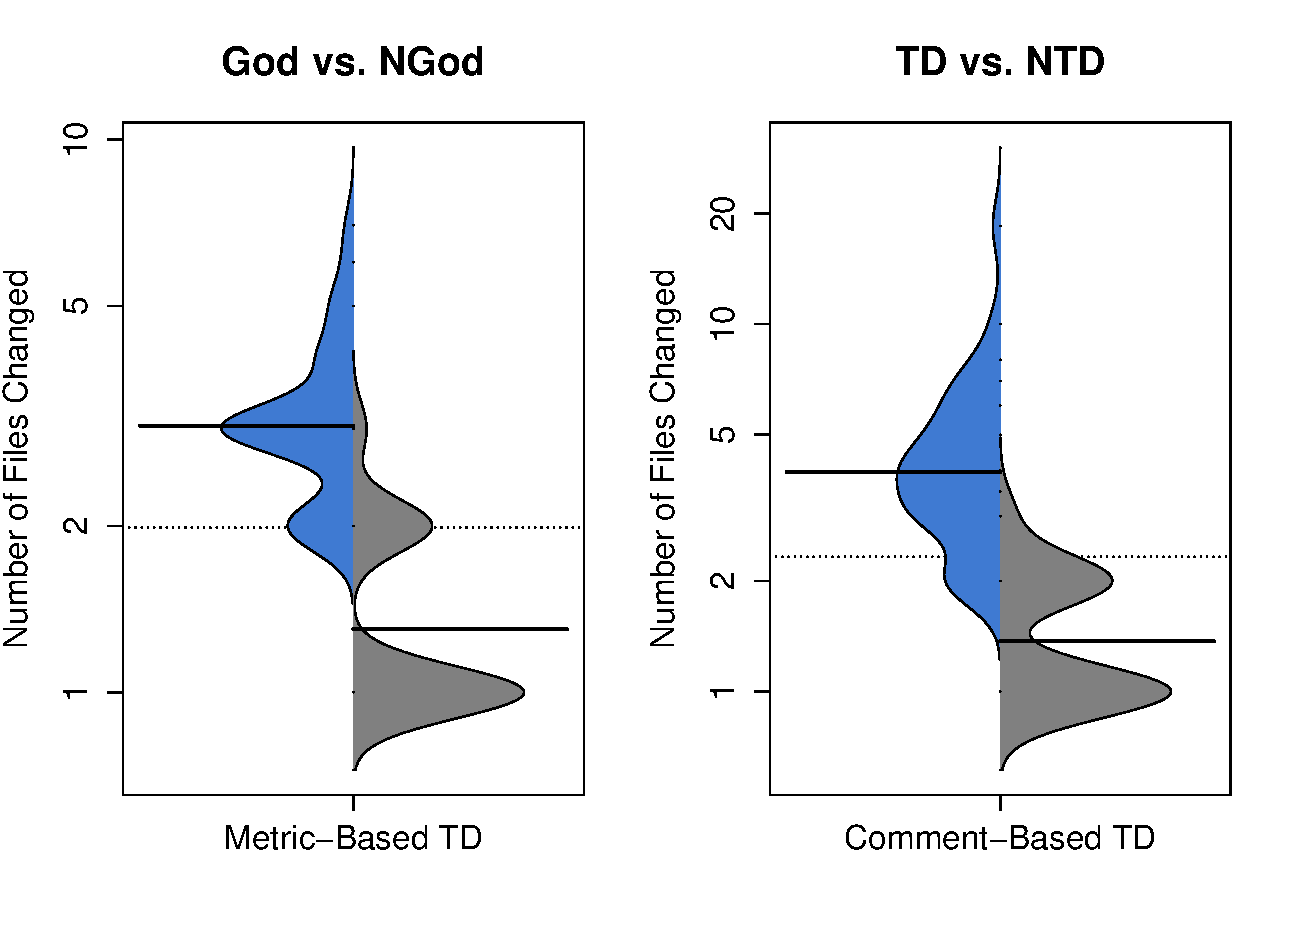
\includegraphics[width=120mm]{figures/chapter4/rq3_nf}
	\caption{Total number of files modified per change for (i) God vs. non-God and (ii) SATD vs. NSATD.}
	\label{figure:ch4_tfcpc}
\end{figure}

\begin{figure}[!hp]
	\centering
	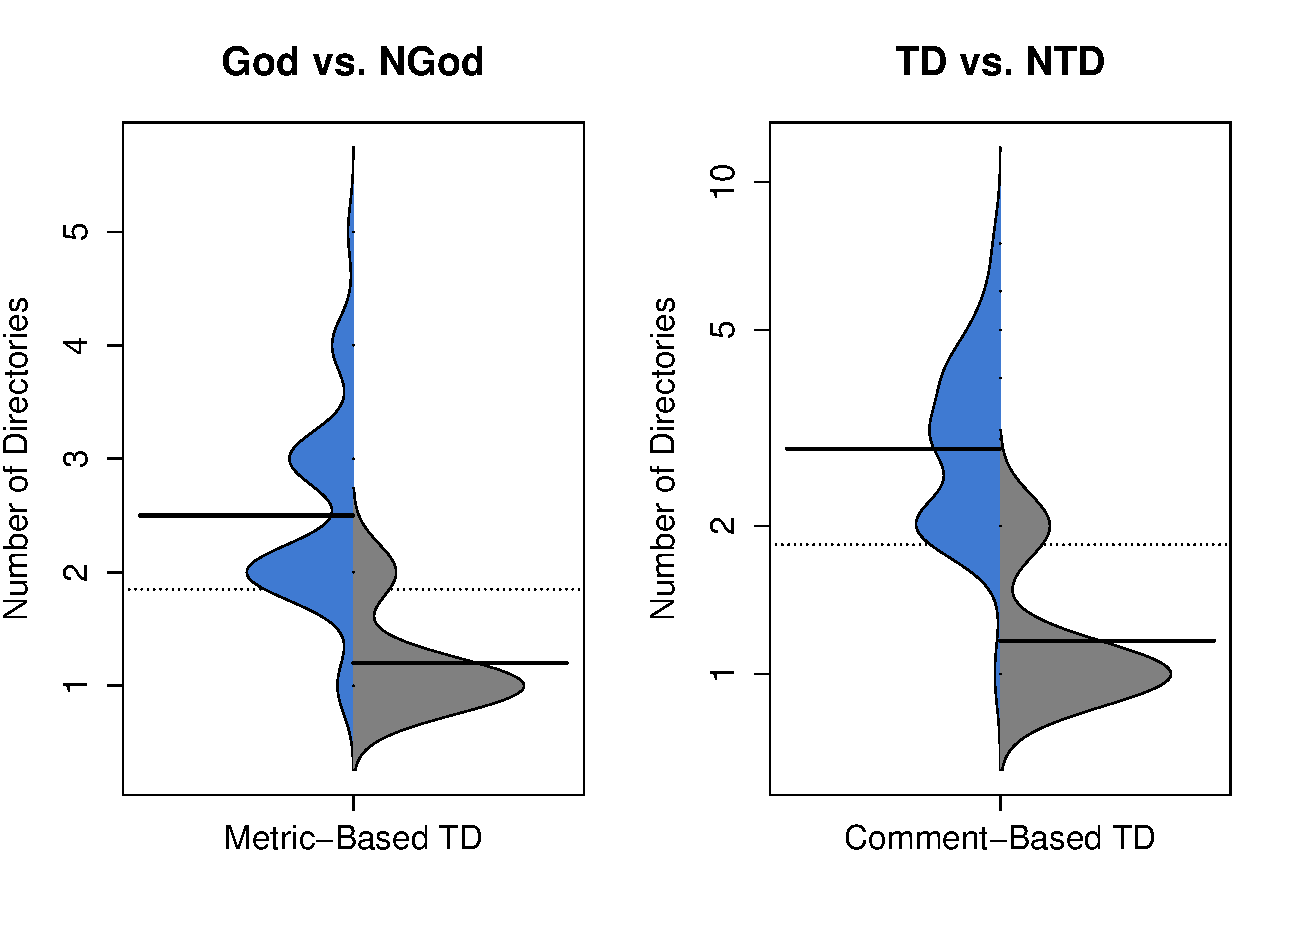
\includegraphics[width=120mm]{figures/chapter4/rq3_nd}
	\caption{Total number of modified directories per change for (i) God vs. non-God and (ii) SATD vs. NSATD.}
	\label{figure:ch4_number_of_directories}
\end{figure}



\begin{figure}[!hp]
	\centering
	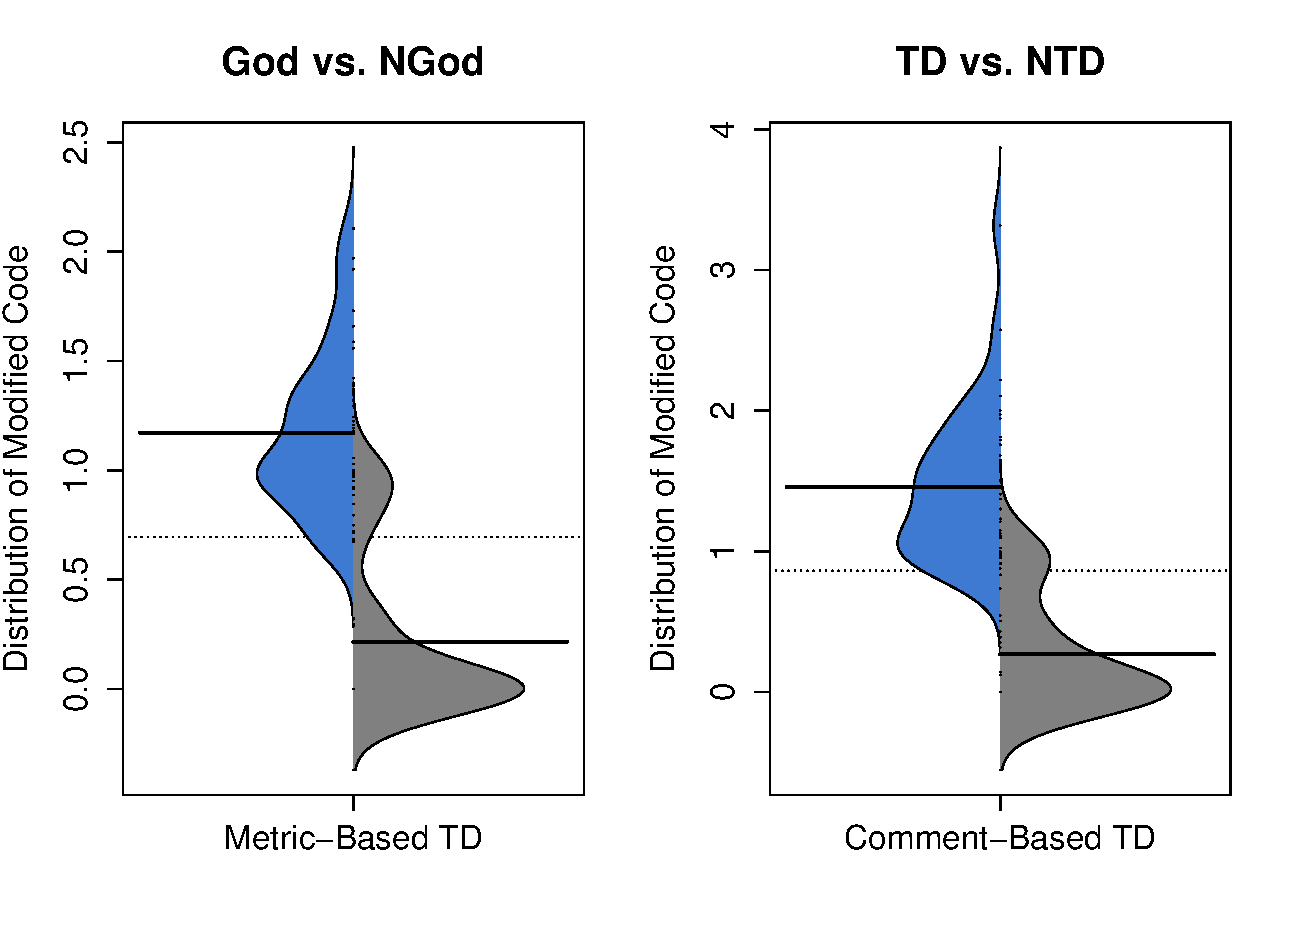
\includegraphics[width=120mm]{figures/chapter4/rq3_entropy}
	\caption{Distribution of the change across files for (i) God vs. non-God and (ii) SATD vs. NSATD.}
	\label{figure:ch4_mtdocatdf}
\end{figure}



%We adopt Hassan's change complexity measure~\cite{hassan2009predicting} to calculate change entropy, defined as $H(P)=-\sum _{k=1}^{n}\textrm ({p}_{k}*{log}_{2} {p}_{k})$, where $k$ is the proportion file$_{k}$ is modified in a change and $n$ is the number of files in the change. Entropy measures the distribution of a change across files. If we consider a change involving modification of three files \textit{A, B} and \textit{C}, for example, and take the number of lines modified to be 30, 1 and 1, respectively, the entropy equates to $0.40=-\frac{30}{32}\log_{2}\frac{30}{32}-\frac{1}{32}\log_{2}\frac{1}{32}-\frac{1}{32}\log_{2}\frac{1}{32}$.

%The maximum entropy $log_{2}n$ has normalized the entropy formula presented above following Hassan~\cite{hassan2009predicting} so that entropy can be compared for changes touching different numbers of files. The higher the normalized entropy, the more difficult it is to make the change.\\

\noindent{\textbf{Results:}}
In each one of Figures~\ref{figure:ch4_tlcpc},~\ref{figure:ch4_tfcpc},~\ref{figure:ch4_number_of_directories} and~\ref{figure:ch4_mtdocatdf}, a distribution is compiled for god and non-god and SATD and non-SATD changes by plotting the median values obtained from a different difficulty measure for each project. Juxtaposition of the \textit{distribution medians} demonstrates that regardless of the metric employed to quantify change difficulty, god and SATD changes are consistently more difficult to perform than non-god and non-SATD changes. Moreover, the Mann-Whitney test \cite{mann1947test} yields $p \le 0.05$, indicating that the differences are statistically significant. Tables~\ref{table:cliff_deltas_RQ4_God} and ~\ref{table:cliff_deltas_RQ4_TD} show the Cliff's delta ~\cite{Cliff:2005} effect size values for all projects studied for both god and SATD changes. We observe that for most projects and all measures of difficulty, the effect size is either medium or large, except for \textit{Hbase, Hama, Deltaspike, Calcite and Stanbol} for god changes and \textit{Hbase and Deltaspike} for SATD changes, which have a small effect size.\\

\begin{landscape}
	\begin{table}[!htbp]

	\small
	\centering


	
	\begin{tabular}{l|c|c|c|c}
		\hline
		\textbf{Project}   & {\bf NF}    & {\bf E} & {\bf C} & {\bf ND}    \\ \hline
\textbf{Apache openNLP} & 0.31 & 0.30 & 0.35 & 0.36\\ \hline
\textbf{Apache Camel} & 0.42 & 0.41 & 0.39 & 0.37\\ \hline
\textbf{Apache Hbase} & 0.23 & 0.24 & 0.29 & 0.22\\ \hline
\textbf{Apache Groovy} & 0.36 & 0.33 & 0.34 & 0.40\\ \hline
\textbf{Apache Oltu} & 0.49 & 0.47 & 0.43 & 0.48\\ \hline
\textbf{Apache Maven} & 0.35 & 0.34 & 0.33 & 0.33\\ \hline
\textbf{Apache Karaf} & 0.29 & 0.26 & 0.36 & 0.27\\ \hline
\textbf{Apache Hama} & 0.27 & 0.25 & 0.32 & 0.22\\ \hline
\textbf{Apache Tomee} & 0.36 & 0.34 & 0.36 & 0.35\\ \hline
\textbf{Apache Deltaspike} & 0.30 & 0.28 & 0.29 & 0.29\\ \hline
\textbf{Apache Curator} & 0.22 & 0.33 & 0.45 & 0.33\\ \hline
\textbf{Apache Calcite} & 0.22 & 0.24 & 0.23 & 0.27\\ \hline
\textbf{Apache Poi} & 0.44 & 0.42 & 0.36 & 0.49\\ \hline
\textbf{Apache Zeppelin} & 0.44 & 0.42 & 0.44 & 0.46\\ \hline
\textbf{Apache Ant} & 0.47 & 0.45 & 0.43 & 0.49\\ \hline
\textbf{Apache Stanbol} & 0.27 & 0.25 & 0.30 & 0.24\\ \hline
\textbf{Apache Kafka} & 0.35 & 0.34 & 0.33 & 0.35\\ \hline
\textbf{Apache Tika} & 0.35 & 0.33 & 0.33 & 0.36\\ \hline
\textbf{Apache Felix} & 0.37 & 0.35 & 0.34 & 0.30\\ \hline
\textbf{Apache Phoenix} & 0.50 & 0.45 & 0.47 & 0.54\\ \hline
\end{tabular}
\quad \quad \quad 
	\begin{tabular}{l|c|c|c|c}
	\hline
	\textbf{Project}   & {\bf NF}    & {\bf E} & {\bf C} & {\bf ND}    \\ \hline

\textbf{Apache Wicket} & 0.58 & 0.58 & 0.55 & 0.53\\ \hline
\textbf{Apache Aurora} & 0.50 & 0.49 & 0.45 & 0.57\\ \hline
\textbf{Apache Ignite} & 0.52 & 0.39 & 0.52 & 0.53\\ \hline
\textbf{Apache Helix} & 0.45 & 0.42 & 0.47 & 0.43\\ \hline
\textbf{Apache Archiva} & 0.39 & 0.39 & 0.38 & 0.30\\ \hline
\textbf{Apache Struts} & 0.40 & 0.48 & 0.43 & 0.43\\ \hline
\textbf{Apache Derby} & 0.54 & 0.53 & 0.52 & 0.52\\ \hline
\textbf{Apache Ambari} & 0.34 & 0.32 & 0.41 & 0.33\\ \hline
\textbf{Apache Nifi} & 0.40 & 0.37 & 0.43 & 0.44\\ \hline
\textbf{Apache Tiles} & 0.30 & 0.29 & 0.29 & 0.36\\ \hline
\textbf{Apache Shiro} & 0.36 & 0.34 & 0.38 & 0.39\\ \hline
\textbf{Apache Usergrid} & 0.50 & 0.43 & 0.46 & 0.52\\ \hline
\textbf{Apache Nutch} & 0.32 & 0.34 & 0.31 & 0.40\\ \hline
\textbf{Apache Zookeeper} & 0.31 & 0.26 & 0.27 & 0.45\\ \hline
\textbf{Apache Mina} & 0.42 & 0.39 & 0.40 & 0.43\\ \hline
\textbf{Apache Cxf} & 0.56 & 0.54 & 0.56 & 0.55\\ \hline
\textbf{Apache Cloudstack} & 0.37 & 0.34 & 0.36 & 0.44\\ \hline
\textbf{Apache Oozie} & 0.52 & 0.47 & 0.47 & 0.60\\ \hline
\textbf{Apache Kylin} & 0.36 & 0.30 & 0.35 & 0.38\\ \hline
\textbf{Apache Flink} & 0.53 & 0.51 & 0.57 & 0.59\\ \hline



	\end{tabular}
		\caption{Cliff's delta for the change difficulty measures across the projects for God Changes.}
		\label{table:cliff_deltas_RQ4_God}
\end{table}
\end{landscape}


\begin{landscape}
	\begin{table}[!htbp]
		
		\small
		\centering
		
		
		
		\begin{tabular}{l|c|c|c|c}
			\hline
			\textbf{Project}   & {\bf NF}    & {\bf E} & {\bf C} & {\bf ND}    \\ \hline
			\textbf{Apache openNLP} & 0.34 & 0.33 & 0.36 & 0.39\\ \hline
			\textbf{Apache Camel} & 0.44 & 0.42 & 0.38 & 0.40
\\ \hline
			\textbf{Apache Hbase} & 0.26 & 0.27 & 0.29 & 0.24
\\ \hline
			\textbf{Apache Groovy} & 0.35 & 0.32 & 0.33 & 0.39
\\ \hline
			\textbf{Apache Oltu} & 0.36 & 0.33 & 0.41 & 0.35\\ \hline
			\textbf{Apache Maven} & 0.40 & 0.39 & 0.37 & 0.38
\\ \hline
			\textbf{Apache Karaf} & 0.35 & 0.32 & 0.40 & 0.34
\\ \hline
			\textbf{Apache Hama} & 0.34 & 0.31 & 0.37 & 0.28
\\ \hline
			\textbf{Apache Tomee} & 0.35 & 0.33 & 0.34 & 0.34
\\ \hline
			\textbf{Apache Deltaspike} & 0.31 & 0.29 & 0.29 & 0.26
\\ \hline
			\textbf{Apache Curator} & 0.40 & 0.30 & 0.51 & 0.40
\\ \hline
			\textbf{Apache Calcite} & 0.30 & 0.31 & 0.29 & 0.35
\\ \hline
			\textbf{Apache Poi} & 0.48 & 0.47 & 0.37 & 0.51\\ \hline
			\textbf{Apache Zeppelin} & 0.59 & 0.57 & 0.56 & 0.59
\\ \hline
			\textbf{Apache Ant} & 0.41 & 0.49 & 0.47 & 0.49
\\ \hline
			\textbf{Apache Stanbol} & 0.33 & 0.30 & 0.34 & 0.39
\\ \hline
			\textbf{Apache Kafka} & 0.40 & 0.39 & 0.39 & 0.40
\\ \hline
			\textbf{Apache Tika} & 0.37 & 0.33 & 0.30 & 0.38\\ \hline
			\textbf{Apache Felix} & 0.30 & 0.38 & 0.36 & 0.33
\\ \hline
			\textbf{Apache Phoenix} & 0.52 & 0.47 & 0.44 & 0.56\\ \hline
		\end{tabular}
		\quad \quad \quad 
		\begin{tabular}{l|c|c|c|c}
			\hline
			\textbf{Project}   & {\bf NF}    & {\bf E} & {\bf C} & {\bf ND}    \\ \hline
			
			\textbf{Apache Wicket} & 0.47 & 0.47 & 0.40 & 0.43
\\ \hline
			\textbf{Apache Aurora} & 0.52 & 0.51 & 0.48 & 0.59
\\ \hline
			\textbf{Apache Ignite} & 0.53 & 0.60 & 0.53 & 0.56
\\ \hline
			\textbf{Apache Helix} & 0.53 & 0.51 & 0.50 & 0.49
\\ \hline
			\textbf{Apache Archiva} & 0.30 & 0.39 & 0.39 & 0.40
\\ \hline
			\textbf{Apache Struts} & 0.37 & 0.39 & 0.39 & 0.34
\\ \hline
			\textbf{Apache Derby} & 0.37 & 0.36 & 0.32 & 0.34
\\ \hline
			\textbf{Apache Ambari} & 0.38 & 0.36 & 0.44 & 0.38
\\ \hline
			\textbf{Apache Nifi} & 0.57 & 0.55 & 0.53 & 0.59
\\ \hline
			\textbf{Apache Tiles} & 0.57 & 0.56 & 0.43 & 0.52
\\ \hline
			\textbf{Apache Shiro} & 0.35 & 0.39 & 0.35 & 0.36
\\ \hline
			\textbf{Apache Usergrid} & 0.51 & 0.44 & 0.47 & 0.52
\\ \hline
			\textbf{Apache Nutch} & 0.49 & 0.51 & 0.43 & 0.54
\\ \hline
			\textbf{Apache Zookeeper} & 0.39 & 0.35 & 0.33 & 0.47
\\ \hline
			\textbf{Apache Mina} & 0.54 & 0.49 & 0.47 & 0.51
\\ \hline
			\textbf{Apache Cxf} & 0.36 & 0.34 & 0.31 & 0.35 \\ \hline
			\textbf{Apache Cloudstack} & 0.40 & 0.37 & 0.29 & 0.46
\\ \hline
			\textbf{Apache Oozie} & 0.53 & 0.50 & 0.45 & 0.57
\\ \hline
			\textbf{Apache Kylin} & 0.57 & 0.52 & 0.53 & 0.59
\\ \hline
			\textbf{Apache Flink} & 0.47 & 0.44 & 0.39 & 0.49 \\ \hline
			
			
			
		\end{tabular}
		\caption{Cliff's delta for the change difficulty measures across the projects for SATD Changes.}
		\label{table:cliff_deltas_RQ4_TD}
	\end{table}
\end{landscape}

\begin{myboxii}[RQ3 - Interim Summary]
	God class-related changes and SATD-related changes are more difficult to perform than non-god and non-SATD changes.
\end{myboxii}

Upon inspection of the boxplots in Figures~\ref{figure:total_number_of_lines_changed_god_vs_ngod},~\ref{figure:total_number_of_lines_changed_td_vs_ntd},~\ref{figure:total_nd_changed_god_vs_ngod},~\ref{figure:total_nd_changed_td_vs_ntd},~\ref{figure:total_files_god_vs_ngod},~\ref{figure:total_files_td_vs_ntd},~\ref{figure:total_entropy_god_vs_ngod} and~\ref{figure:total_entropy_td_vs_ntd} (in appendix), we find that the distribution median and distribution mean inequalities remain unchanged for all projects for all difficulty measures except for number of directories in OpenNLP, where non-god and non-SATD change medians are still not greater than those of god and SATD changes, but about equal. In summary, then, performing god and SATD changes is more difficult than performing non-god and non-SATD changes by all difficulty measures.


\subsection*{\chapterIVrqIV}

%\todo{finish this research question}


\noindent{\textbf{Motivation:}}
Thus far, we have compared how the technical debt identified by comment- and metric-based approaches relates to software quality. What remains outstanding now is the amount of overlap between the \SATD files that the comment-based approach labels and the god files that the metric-based approach detects. Specifically, our objective is to calculate the percentage of files that contain technical debt on both counts so that we can garner a better understanding of how comment-based technical debt complements metric-based technical debt.


\noindent{\textbf{Approach:}}
We take the list of \SATD files generated by the comment-based approach and the list of god files generated by the metric-based approach and isolate the files that made both lists. We count how many of these files meet the criteria for both approaches and then divide by the total number of files in both lists. The result represents the share of comment-based technical debt that complements metric-based technical debt (overlap), expressed as a percentage.


\noindent{\textbf{Results:}}

Table~\ref{ch4_amount_of_overlap} displays the percentage overlap by project. We see that the values range from 11\% to 34\%. Our findings confirm that the comment-based approach, which uses source code comment patterns to detect technical debt, complements the metric-based approach, which relies on thresholds of object-oriented metrics. In other work, Moldonado \textit{et al.} \cite{Maldonado_TSE2017} studied the overlap between \SATD and several types of code smells extracted by a static analysis tool for 10 open-source projects. For \SATD and god classes specifically, they found an average overlap of 44.2\%, which, though higher than the overlap we found, is based on a smaller sample size. Despite considerable overlap, each of the comment- and metric-based approaches identifies some additional sources of technical debt that the other fails to detect.

\begin{myboxii}[RQ4 - Interim Summary]
	The comment-based approach complements the metric-based approach with an overlap ranging from 11\% to 34\%. Nevertheless, practitioners should integrate both approaches in order to better detect technical debt.
\end{myboxii}

	\begin{table}[!htbp]
	\small
	\centering
	
	\begin{tabular}{l|c}
		\hline
		\textbf{Project}           & \textbf{Overlap (\%)} \\ \hline
		\textbf{Apache OpenNLP}    &    24.39     \\ \hline
		\textbf{Apache Camel}      &    16.57     \\ \hline
		\textbf{Apache Habse}      &    33.88     \\ \hline
		\textbf{Apache Groovy}     &    30.10     \\ \hline
		\textbf{Apache Oltu}       &    16.68     \\ \hline
		\textbf{Apache Maven}      &    26.08     \\ \hline
		\textbf{Apache Karaf}      &    23.65     \\ \hline
		\textbf{Apache Hama}       &    29.51     \\ \hline
		\textbf{Apache Tomee}      &    21.61     \\ \hline
		\textbf{Apache Deltaspike} &    20.46     \\ \hline
		\textbf{Apache Curator}    &    25.23     \\ \hline
		\textbf{Apache Calcite}    &    31.12     \\ \hline
		\textbf{Apache Poi}        &    31.36     \\ \hline
		\textbf{Apache Zeppelin}   &    23.37     \\ \hline
		\textbf{Apache Ant}        &    28.86     \\ \hline
		\textbf{Apache Stanbol}    &    32.95     \\ \hline
		\textbf{Apache Kafka}      &    20.64     \\ \hline
		\textbf{Apache Tika}       &    33.56     \\ \hline
		\textbf{Apache Felix}      &    26.00     \\ \hline
		\textbf{Apache Phoenix}    &    30.99     \\ \hline
	\end{tabular}
	\quad \quad \quad
	\begin{tabular}{l|c}
		\hline
		\textbf{Project}           & \textbf{Overlap (\%)} \\ \hline
		\textbf{Apache Wicket}     &    19.33     \\ \hline
		\textbf{Apache Aurora}     &    26.44     \\ \hline
		\textbf{Apache Ignite}     &    14.28     \\ \hline
		\textbf{Apache Helix}      &    25.45     \\ \hline
		\textbf{Apache Archiva}    &    30.33     \\ \hline
		\textbf{Apache Struts}     &    24.74     \\ \hline
		\textbf{Apache Derby}      &    32.56     \\ \hline
		\textbf{Apache Ambari}     &    25.59     \\ \hline
		\textbf{Apache Nifi}       &    18.92     \\ \hline
		\textbf{Apache Tiles}      &    11.37     \\ \hline
		\textbf{Apache Shiro}      &    31.03     \\ \hline
		\textbf{Apache Usergrid}   &    26.90     \\ \hline
		\textbf{Apache Nutch}      &    32.11     \\ \hline
		\textbf{Apache Zookeeper}  &    26.70     \\ \hline
		\textbf{Apache Mina}       &    16.78     \\ \hline
		\textbf{Apache Cxf}        &    22.25     \\ \hline
		\textbf{Apache CloudStack} &    27.91     \\ \hline
		\textbf{Apache Oozie}      &    21.88     \\ \hline
		\textbf{Apache Kylin}      &    22.54     \\ \hline
		\textbf{Apache Flink}      &    15.37     \\ \hline
	\end{tabular}
	\caption{Percentage of overlap between God and SATD files of the analyzed projects.}
	\label{ch4_amount_of_overlap}
\end{table}

\pagebreak



\section{Threats to Validity}
\label{chap4:sec:threats_to_validity}


Threats to \textbf{internal validity} concern any factors that could have confounded our study results. Since developers might not think to declare the introduction of a technical debt in the first place, or remove the corresponding comment after eliminating a technical debt, one candidate is the use of source code comments. Every time the code and comment do not undergo a change simultaneously, the source code comments become a less and less accurate record. Despite this, Potdar and Shihab~\cite{ICSM_PotdarS14} found that in Eclipse code and comments were updated in tandem between 70\% and 90\% of the time. Another threat derives from comments intended to indicate SATD that do not correspond to any of the patterns Potdar and Shihab~\cite{ICSM_PotdarS14} compiled, which, owing to the flexibility of natural language, had to be analyzed manually. This technique is error-prone and somewhat subjective, in that developers could conceivably disagree as to which comments indicate SATD consistently. To mitigate these effects, we conducted manual inspections of all identified comments for each project in turn to certify that each contained one of the 62 patterns in \cite{ICSM_PotdarS14}. While we chose to identify any change containing at least one SATD file as an SATD change, we could have reserved this label for changes containing only SATD files. In our view, it is better not to restrict SATD changes in this way because sometimes all it takes is one SATD file to change several other files touched by the same change.


Threats to \textbf{external validity} concern the generalizability of our results. In order to optimize this, we analyzed 40 large open-source systems. Nonetheless, other systems should be analyzed to support the conclusions of this chapter, for one thing, because all the projects studied were written in Java, which limits programming language representation. Additionally, the projects studied were all developed by Apache, so systems developed by other companies could potentially run counter to our findings. Drawing on open-source projects means we have no guarantee that our results hold for industrial systems. Moreover, we focused on the relationship between SATD and god classes only, which means that other, unadmitted technical debt or code smells might have been overlooked. Nonetheless, studying all technical debt is beyond the scope of this thesis.

Threats to \textbf{construct validity} concern the extent to which indirect metrics do not accurately measure what they are intended to. Code metrics and thresholds were used to detect god classes as Marinescu \cite{marinescu2004detection} proposes, and while these have proven effective when applied in other studies, it has not been evaluated whether such strategies are suitable to use in all contexts. If not, findings will depend heavily on the particular metrics and thresholds specified for detection and varying these will alter our findings.

%and drew our data from the well-established, mature codebase of open-source software projects with well-commented source code

%We  believe the number of the analyzed systems  is sufficient enough to generalize our results. However,  we cannot be sure  that our findings  will be valid for other domains, applications,  programming languages, or proprietary  projects.

%Furthermore, we focused on SATD and god classes relationship only, which means that we do not cover all technical debt and therefore there may be other technical debt that is not self-admitted or a code smell. Studying all technical debt is beyond the scope of this thesis.





\section{Conclusion}
\label{chap4:sec:conclusion}


The software development community stigmatizes technical debt, even though it still lacks adequate evidence to formalize its adverse effects on software quality. Accordingly, the empirical study we present in this chapter seeks to identify in what ways god classes and self-admitted technical debt detract from quality. God classes centralize the workload of trivial classes and perform tasks using their data in violation of the object-oriented design principle stipulating one task per class. Self-admitted technical debt encompasses bugs that develop over time as a result of resorting to quick fixes that ``do the job" for the deadline and defer associated costs which could jeopardize the code in the long run. We identify god classes by employing Marinescu's \cite{marinescu2004detection} object-oriented metric thresholds and \SATD by locating source code comments that match the SATD indicator patterns in \cite{ICSM_PotdarS14}.


Three correlations allowed us to dissect the relationship between god classes and software quality: (i) whether god files have more defects than non-god files, (ii) whether god changes introduce future defects and (iii) whether god changes are more difficult to perform. Likewise, we examine the relationship between \SATD and quality by determining (i) whether SATD files have more defects than non-SATD files, (ii) whether SATD changes introduce future defects and (iii) whether SATD-related changes are more difficult to perform. We measured change difficulty for both god classes and \SATD in terms of the amount of churn, numbers of files and modified modules in a change and entropy. After dealing with god and SATD files and changes separately, we assess (iv) to what extent the metric- and comment-based approaches overlap.


In the end, we found that (i) there is no dependable trend between god classes or \SATD and defects: three exceptional projects revealed more corrective changes in SATD files than in non-SATD files; (ii) a trend did surface, however, in that both god changes and SATD changes are more correlated with the introduction of future defects and (iii) more difficult to perform than non-god and non-SATD changes. As for the overlap between the two approaches, we learned that (iv) the metric- and comment-based approaches identify the same sources of technical debt in 11\% to 34\% of cases.

Our study imparts that although god classes and technical debt may have detrimental effects, these imply nothing with respect to defects \textit{per se}, but increase the number of defect-inducing changes and make the system more difficult to change in the future. We advise practitioners to integrate both the comment- and metric-based approach to improve technical debt detection.

\chapter{Summary, Contributions and Future Work}
\label{conclusion}
% -*- root: cuthesis_masters.tex -*-

\section{Summary of Addressed Topics}


Chapter 2 offers a synopsis of the latest research on technical debt, which has generated much interest in the software development community in recent years. Consequently, we find it to be an opportune time to pick up where this body of research left off and address some of the inquiries it has not yet delved into, whether not thoroughly enough or not at all. It should do much in the way of informing current debate in the field to determine whether the technical debt metaphor and developers' views of the practice hold up under further scrutiny.

Chapter 3 presents the impact of comment-based technical debt (\SATD) on software quality. In this chapter, we analyze the source code comments of five well-commented open-source projects representing various domains and programming languages that have a large number of contributors. We find that: (i) files with SATD have more defects than files without SATD, (ii) SATD changes are associated with less future defects than non-SATD changes and (iii) SATD changes are more difficult to execute.

Chapter 4 presents the effects of comment- versus metric-based technical debt on software quality. In this chapter, we analyze 40 open-source projects to understand how god classes and \SATD influence software quality. We observe that: (i) neither the incidence of god nor \SATD files is correlated with defects, (ii) future defects are introduced at a higher rate by god and SATD changes, (iii) the difficulty imposed on the system is greater for god and SATD changes and (iv) the comment- and metric-based approaches agree on 11\% to 34\% of identified sources of technical debt.

\section{Contributions}
The major contributions of this thesis are as follows:

\begin{itemize}
		\item A comprehensive review of the state of the art in the technical debt field, noting empirical gaps in the theory that enable interested researchers to focus on the main challenges in the field of technical debt.
		\item Enhance knowledge of the technical debt phenomenon by presenting a large-scale empirical study on comment- and metric-based approaches.
		\item Prevent uninformed assumption of technical debt by exposing the risks associated with the practice.
\end{itemize}
\section{Future Work}

We believe that this thesis advances the state of the art in measuring the impact of technical debt on software quality. Though our research clarifies the dynamics of this complex relationship, there are other dimensions of software quality that should be navigated in order to understand the full force of technical debt's impact.

\subsection{Automating Technical Debt Management}

Our findings lay the groundwork for creating a tool that would assist developers in understanding and mitigating the undesirable long-term consequences of incurring technical debt. We have every reason to believe that a tool of this kind would facilitate detection and management of different varieties of technical debt while enhancing design practices, which would optimize the overall quality of the system and dovetail formerly discrete stages in the development process.


\subsection{Diversifying Code Smell Representation}

The scope of this thesis was not conducive to studying the overlap between \SATD and all instantiations of code smells, yet developers would certainly benefit from further research that demonstrates how code smells besides god classes fit into the picture. The overlap between \SATD and lazy class, black sheep, shotgun surgery, etc. could indicate that comment-based approaches to detecting technical debt are more or less reliable than the respective metric-based approaches.

\subsection{Granularizing Technical Debt Classification}

We have focused our attention so far on the impact of technical debt on software quality at the file and change levels. Naturally, a logical progression would be to accommodate the method level, as it would provide more granular insights into the implications of technical debt for quality as a result of increasing confidence in the organization of files into SATD and non-SATD categories.



\begin{appendices}
	\label{appendix}
	\section{List of Figures}

\begin{figure}[tb]
	\centering
	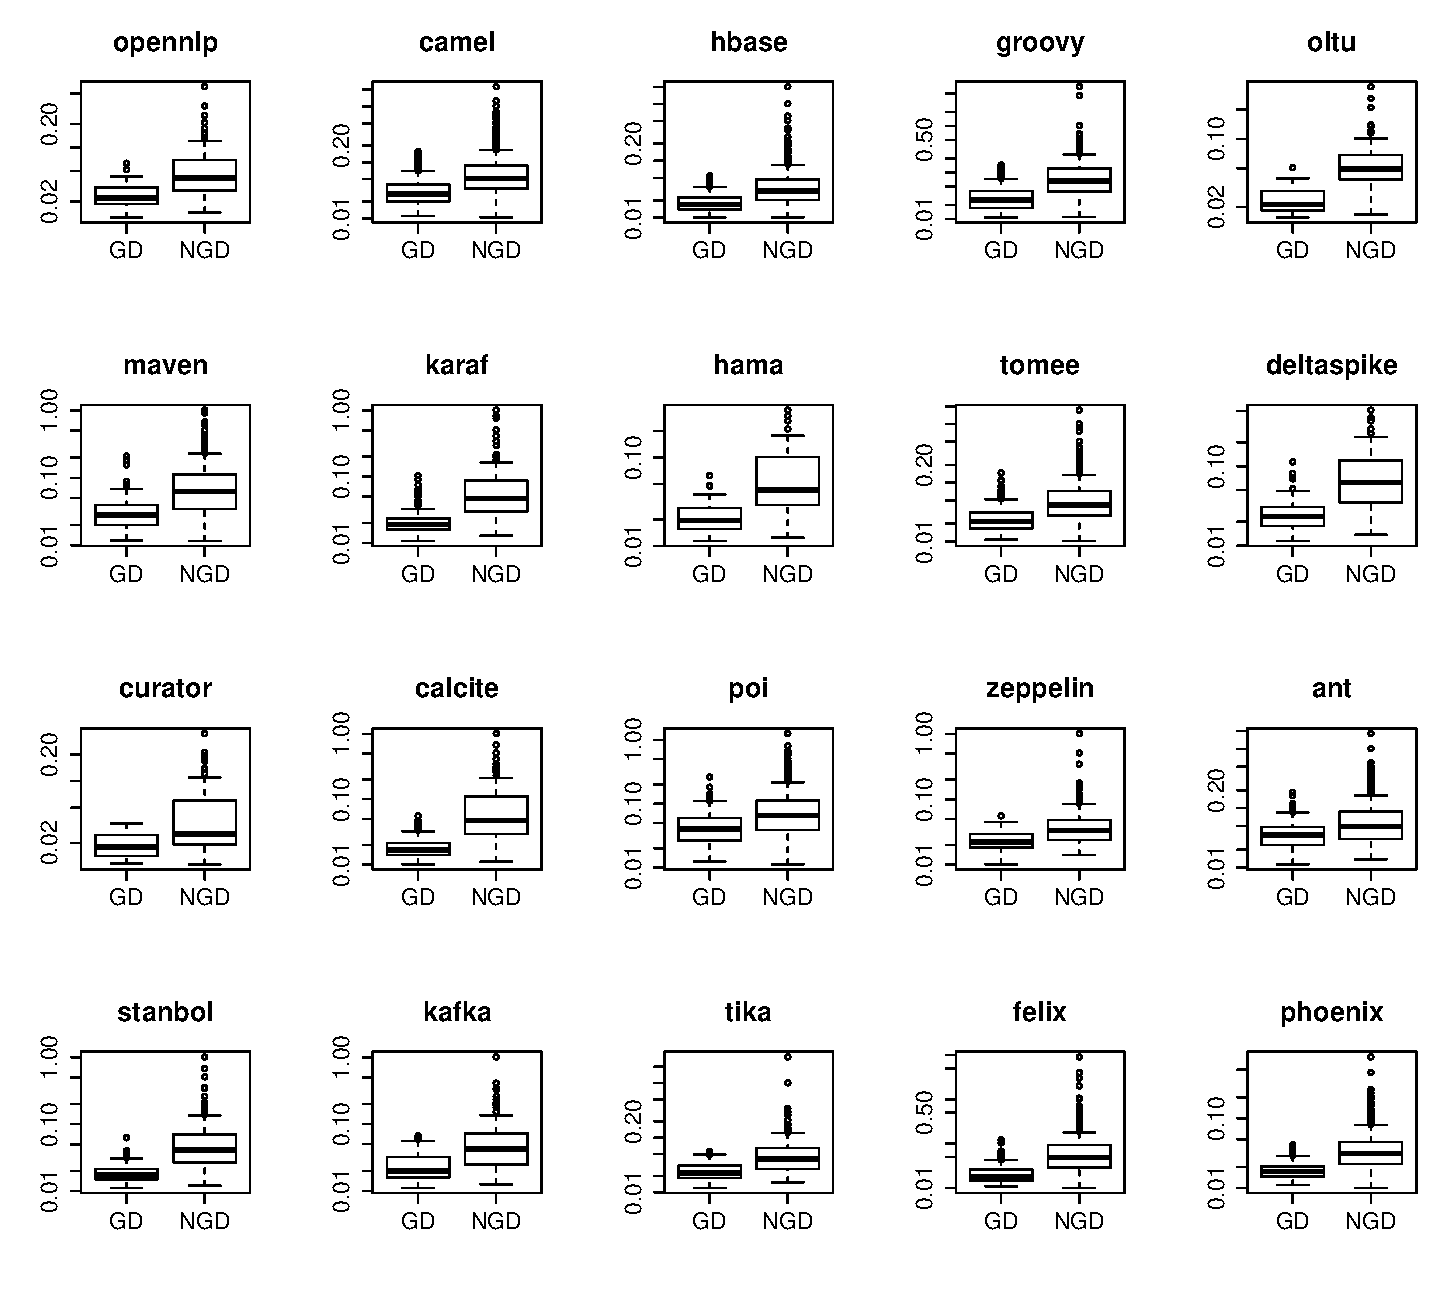
\includegraphics[width=100mm]{figures/chapter4/RQ1_boxplots_god_1}
	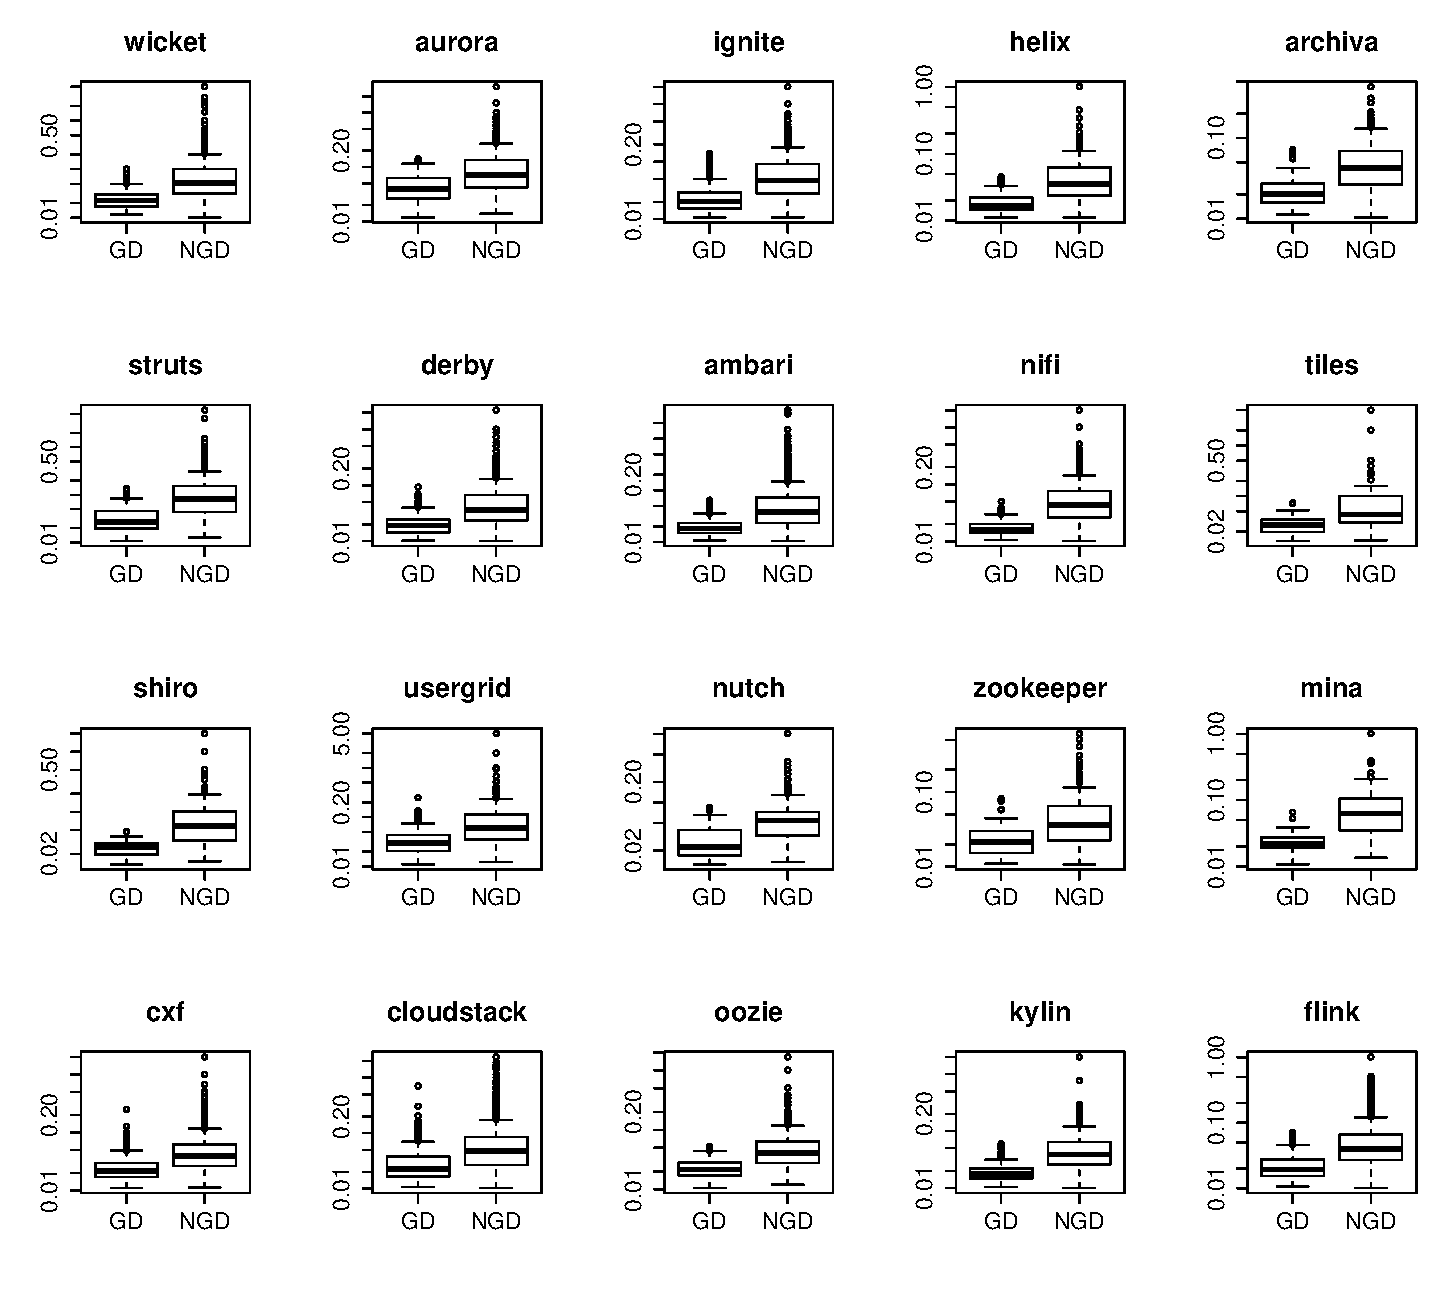
\includegraphics[width=100mm]{figures/chapter4/RQ1_boxplots_god_2}
	\caption{Percentage of defect fixing changes for GOD and NGOD files.}
	\label{figure:percentage_of_defects_god_vs_ngod}
\end{figure}



\begin{figure}[tb]
	\centering
	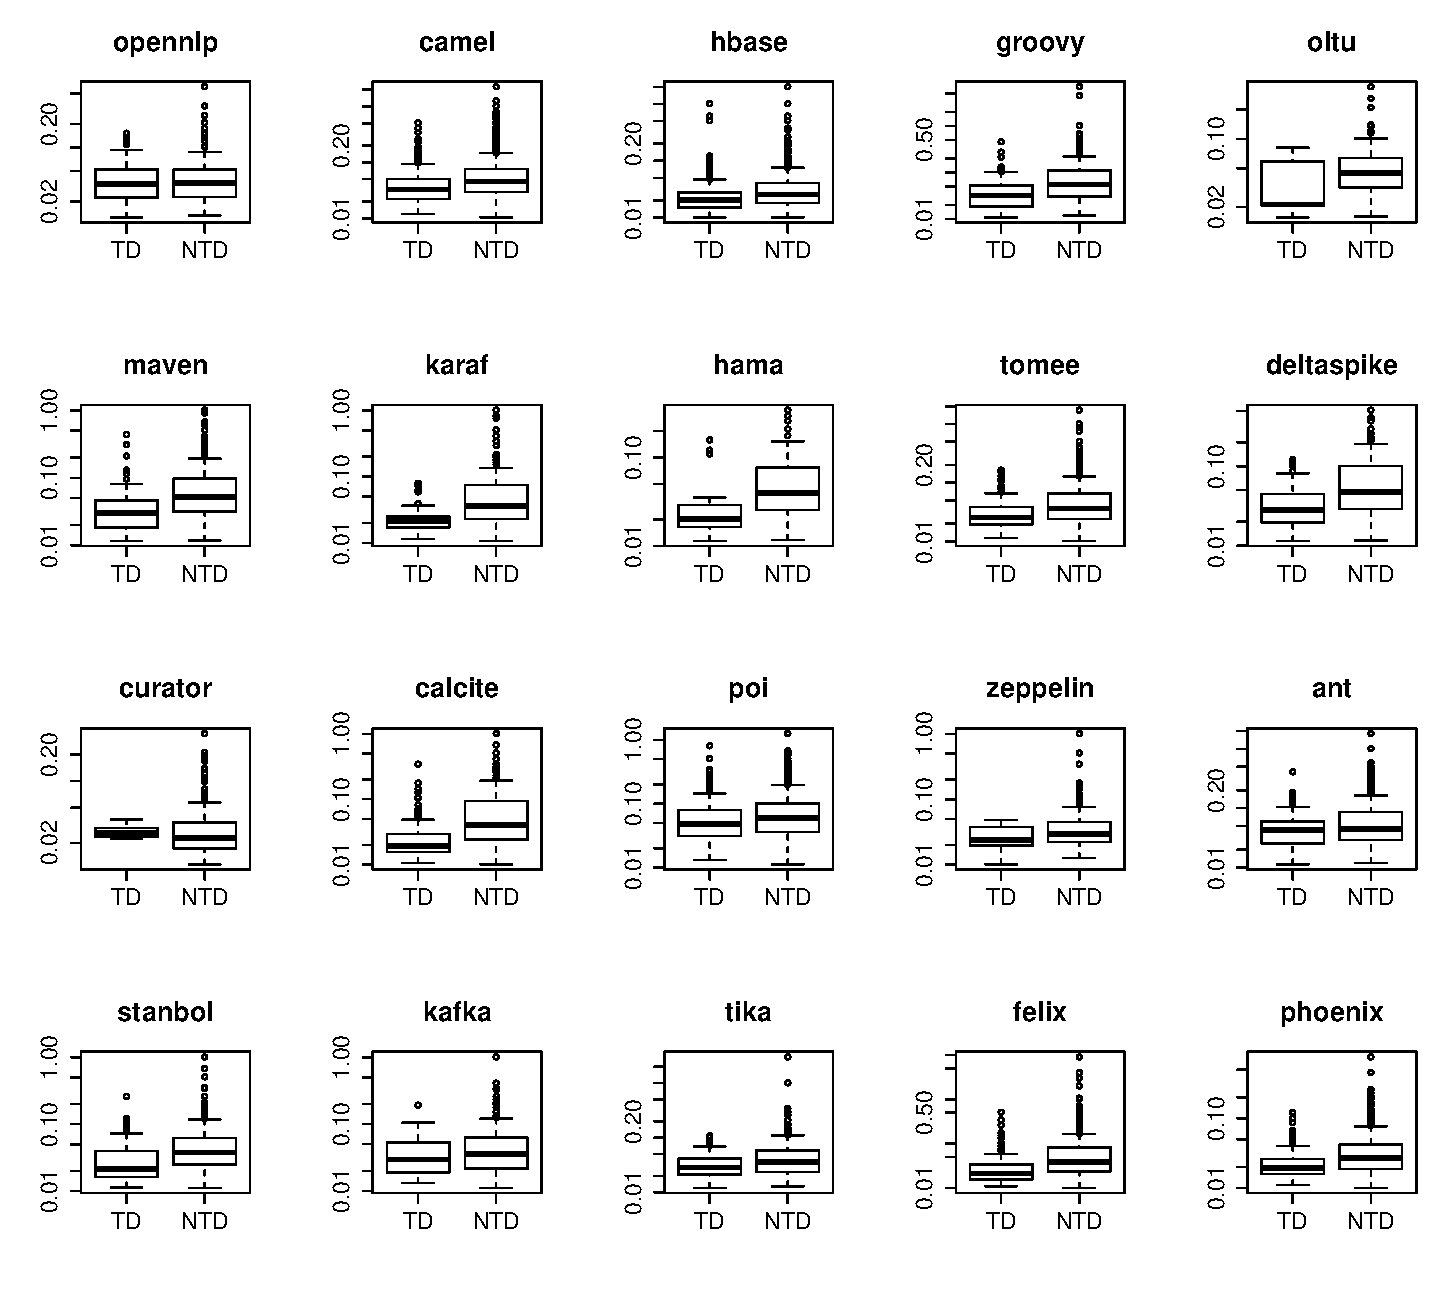
\includegraphics[width=100mm]{figures/chapter4/RQ1_boxplots_td_1}
	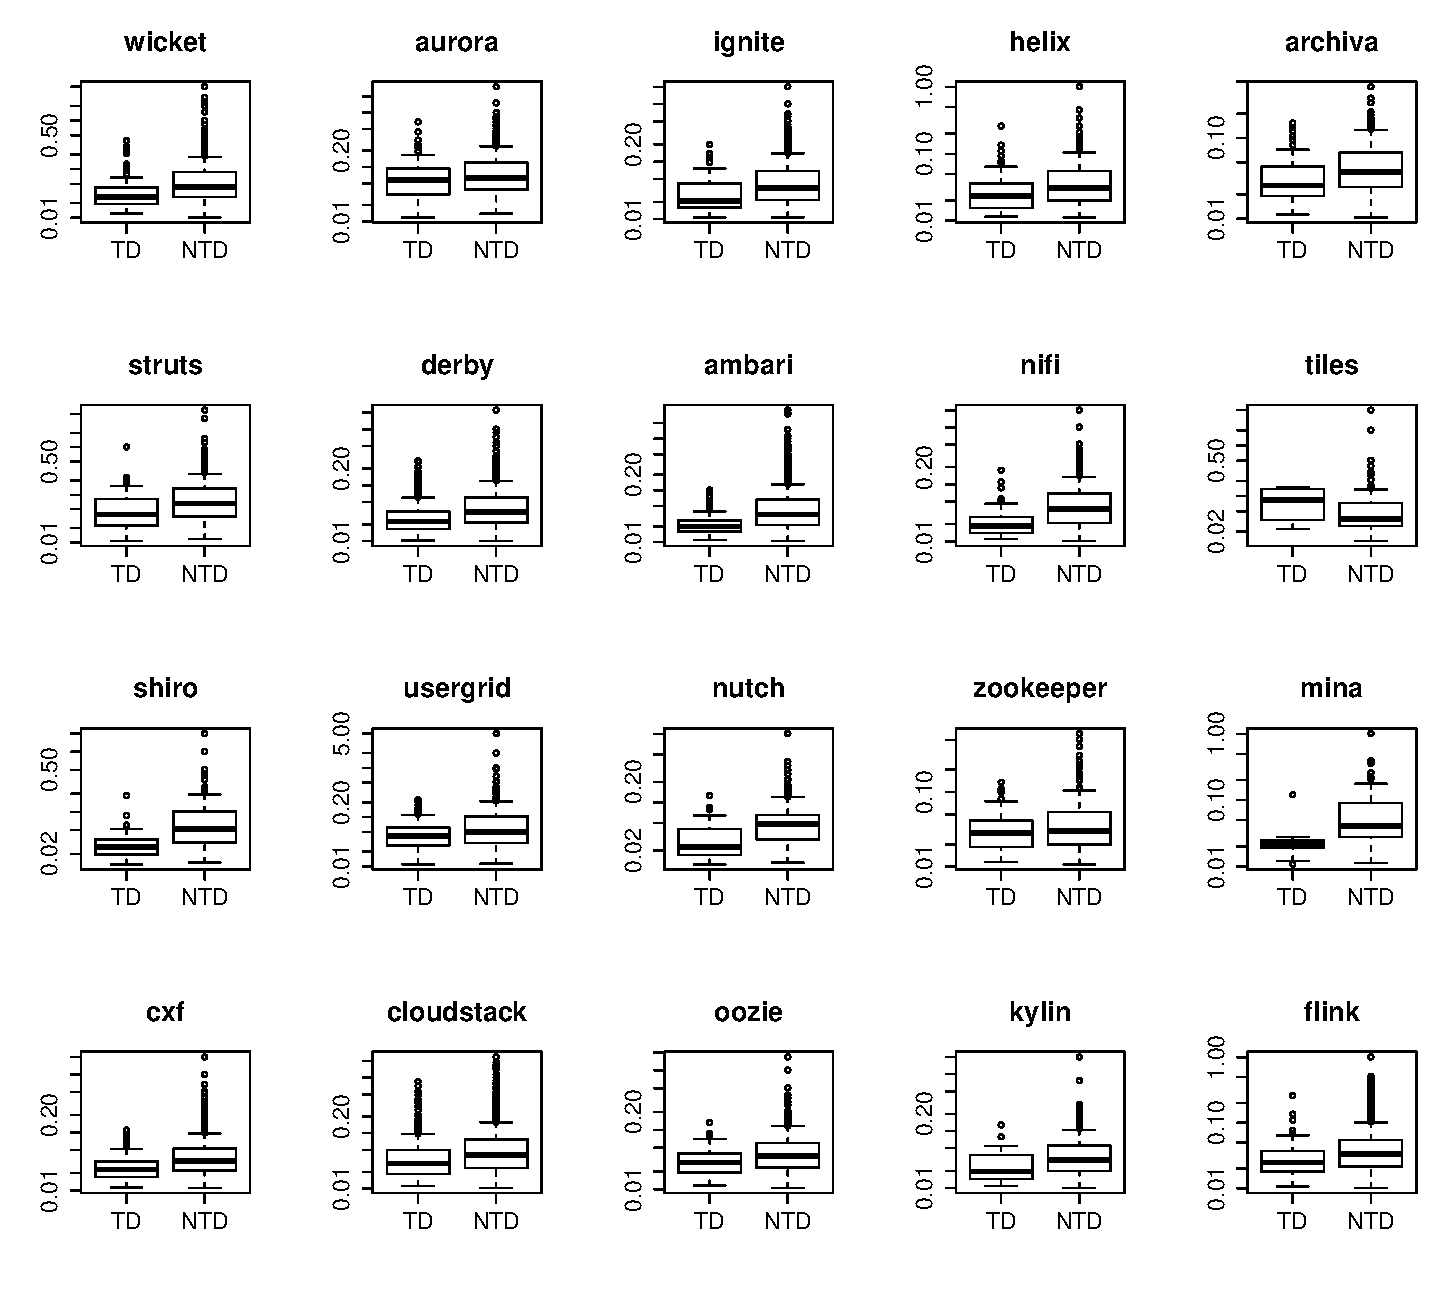
\includegraphics[width=100mm]{figures/chapter4/RQ1_boxplots_td_2}
	\caption{Percentage of defect fixing changes for TD and NTD files.}
	\label{figure:percentage_of_defects_td_vs_ntd}
\end{figure}




\begin{figure}[tb]
	\centering
	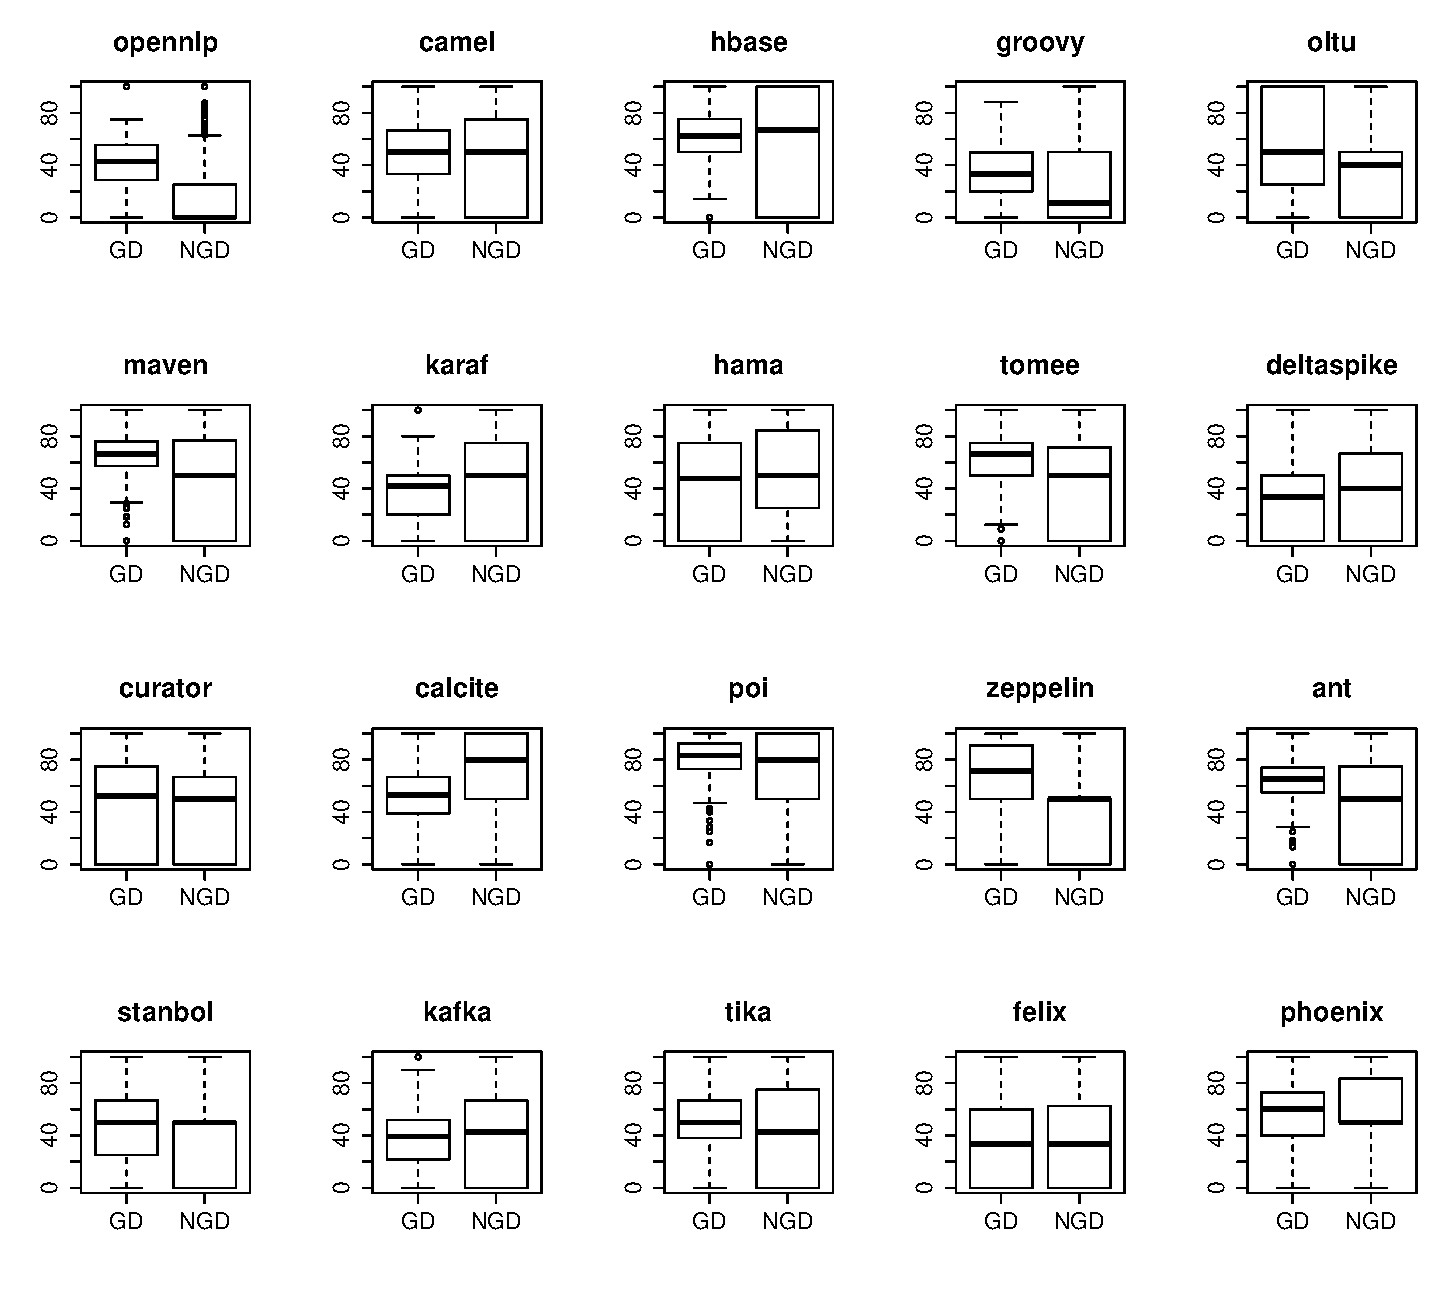
\includegraphics[width=100mm]{figures/chapter4/rq2_god_boxplots_1}
	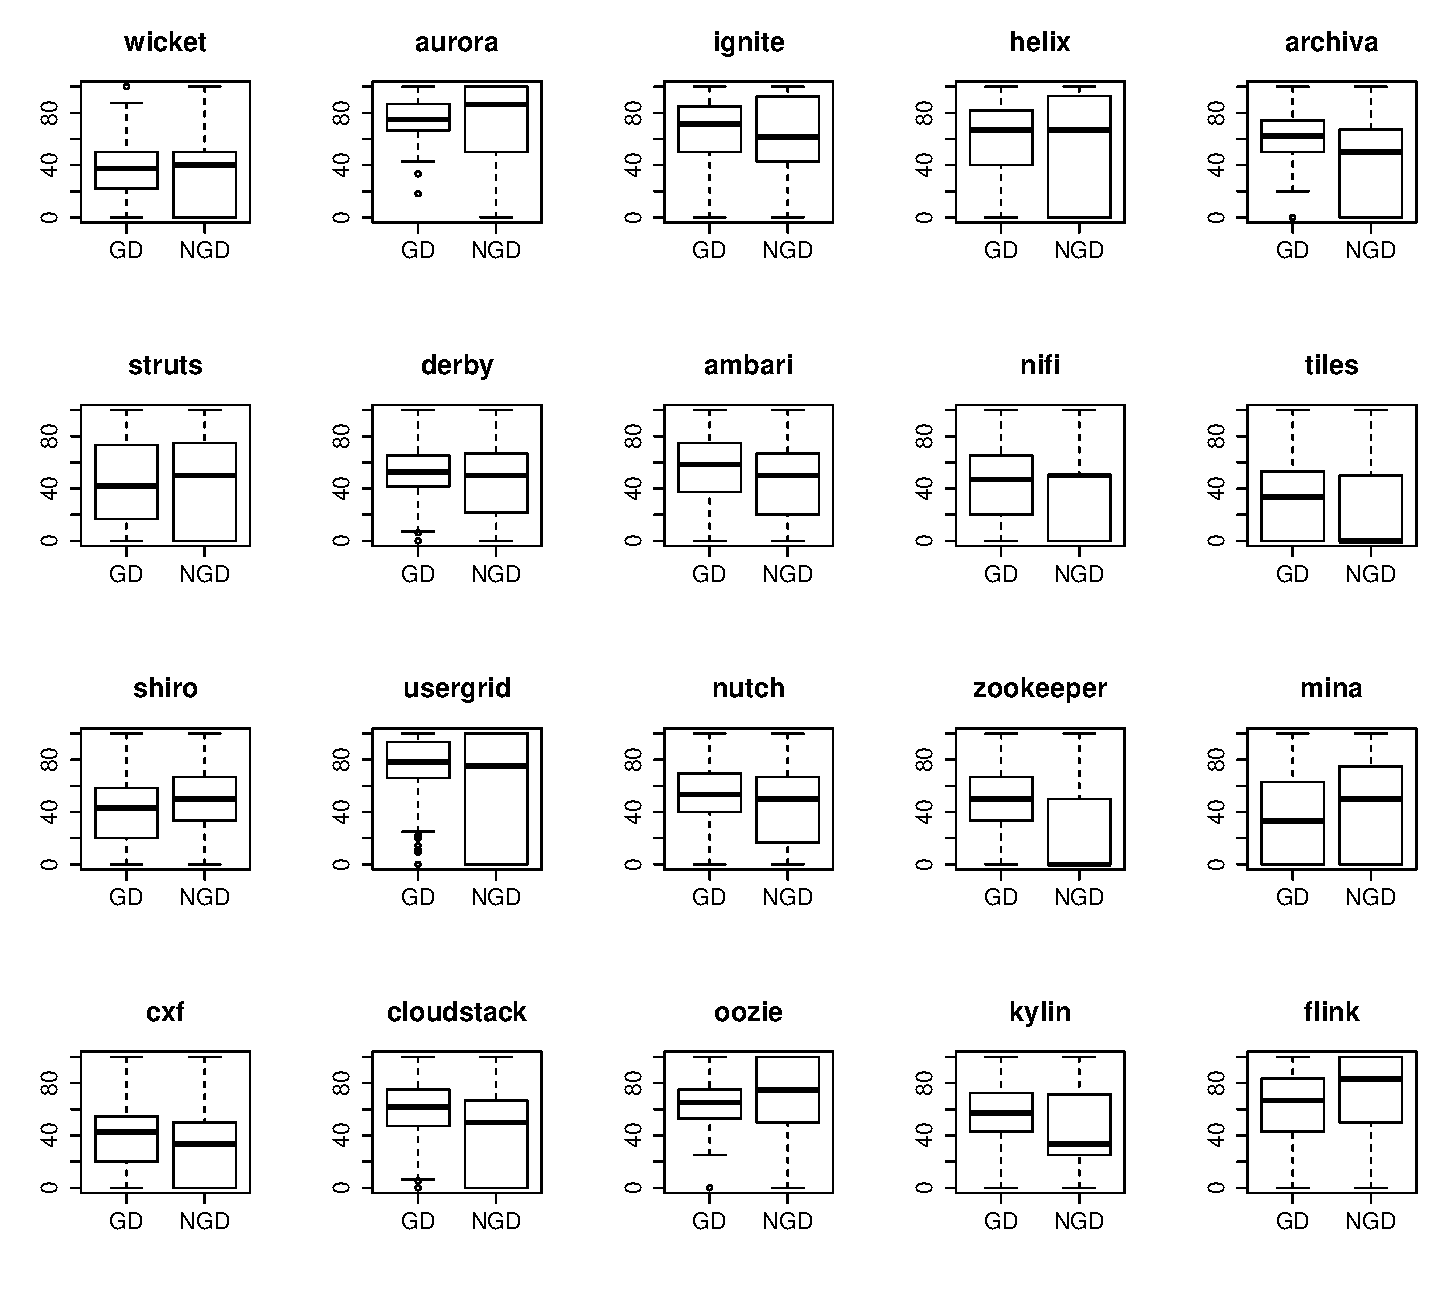
\includegraphics[width=100mm]{figures/chapter4/rq2_god_boxplots_2}
	\caption{Percentage of defect inducing changes for GOD and NGOD files.}
	\label{figure:percentage_of_bug_inducing_god_vs_ngod}
\end{figure}


\begin{figure}[tb]
	\centering
	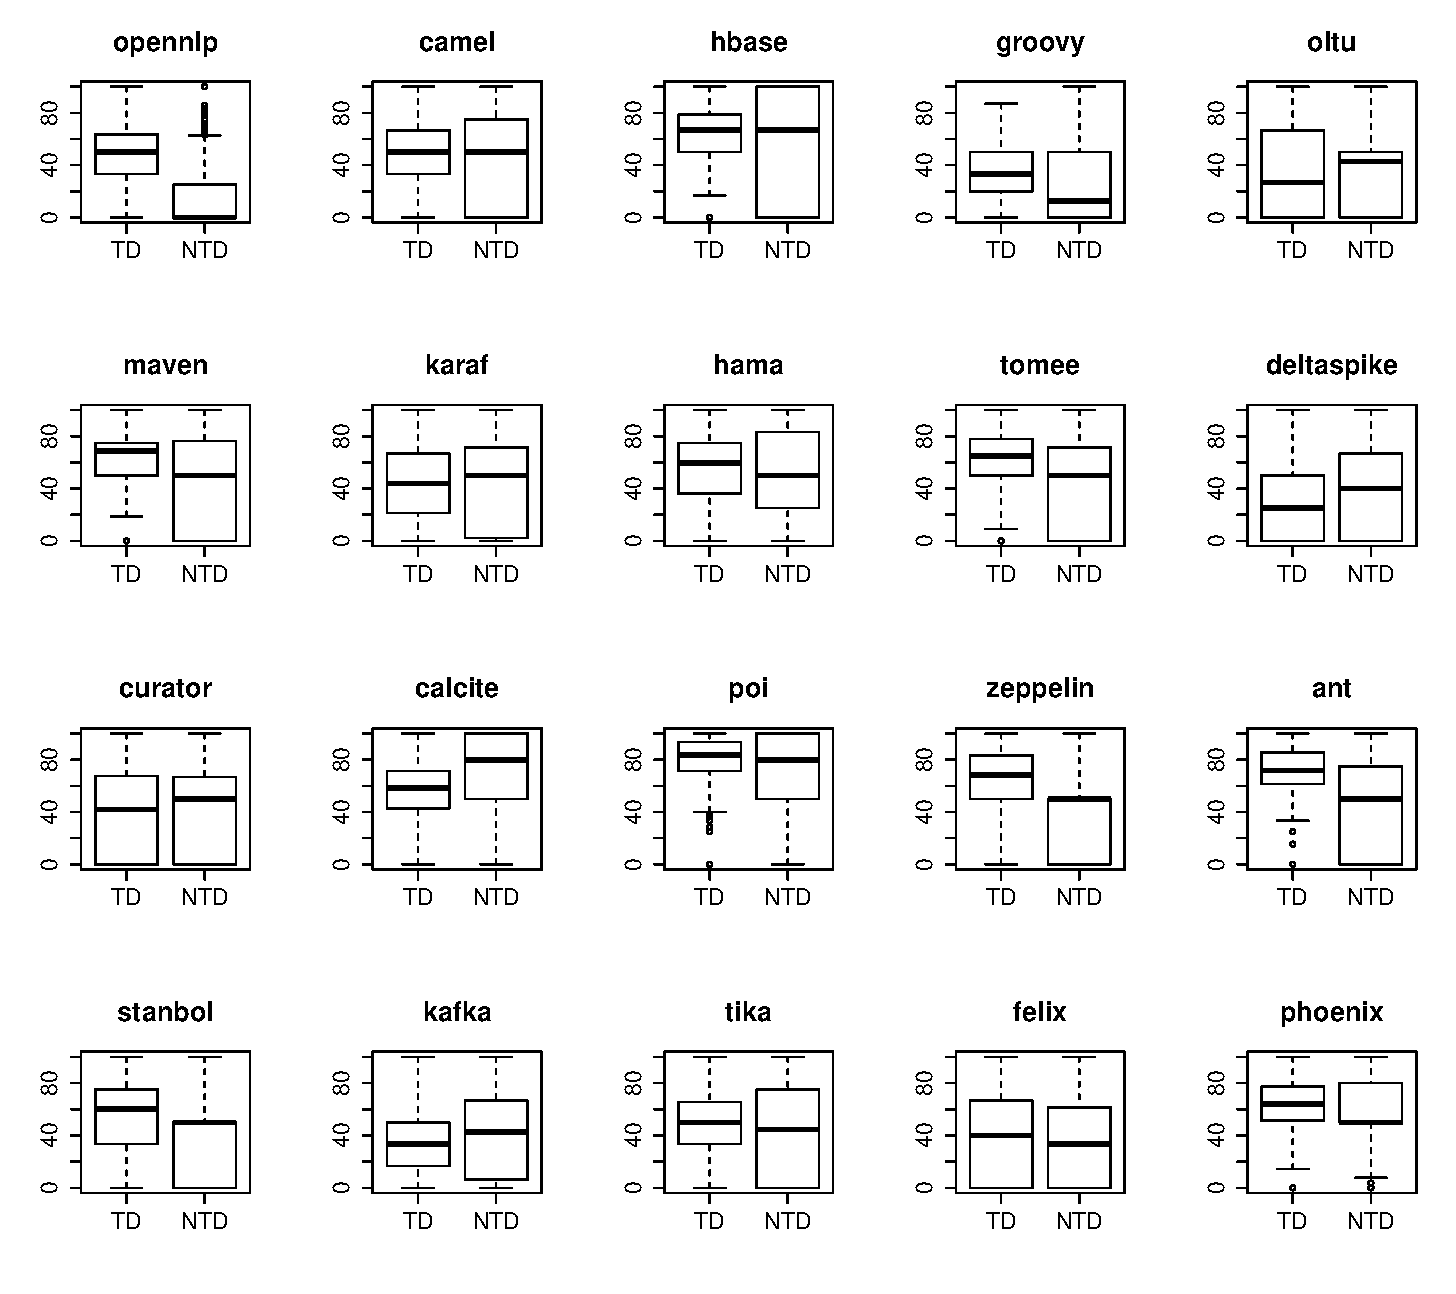
\includegraphics[width=100mm]{figures/chapter4/rq2_boxplots_1}
	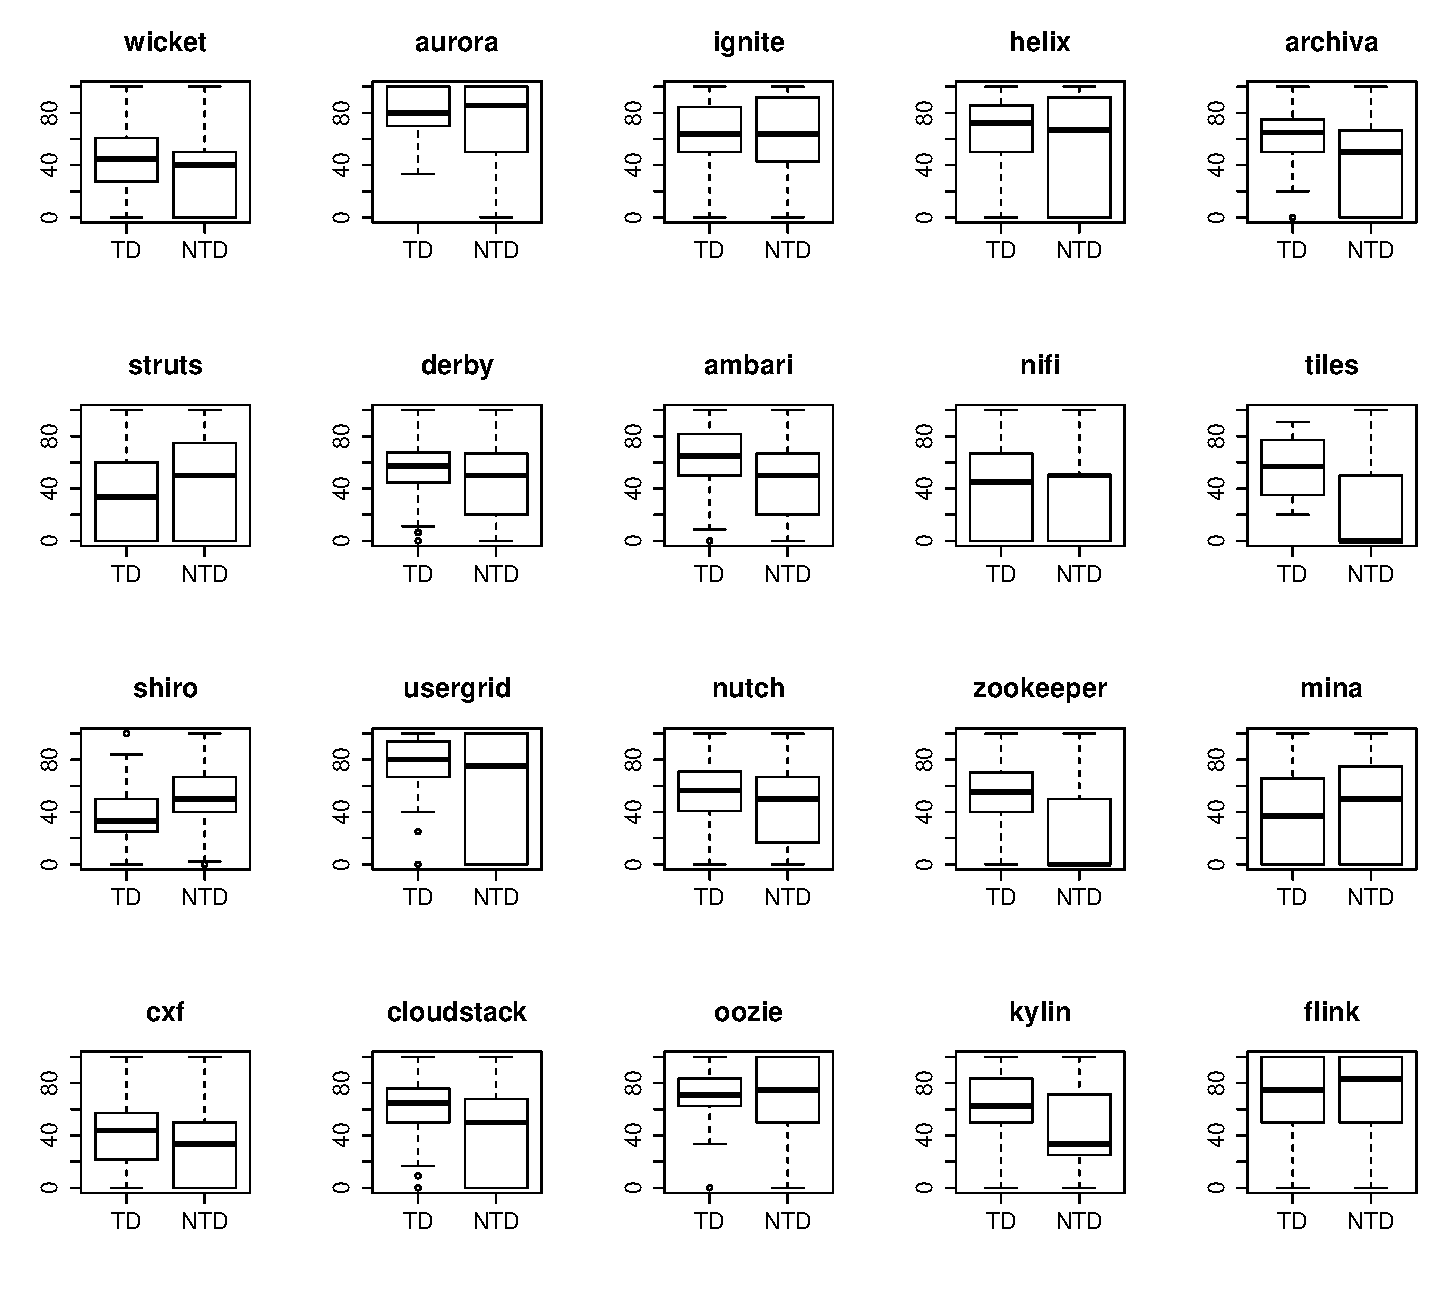
\includegraphics[width=100mm]{figures/chapter4/rq2_boxplots_2}
	\caption{Percentage of defect inducing changes for TD and NTD files.}
	\label{figure:percentage_of_bug_inducing_td_vs_ntd}
\end{figure}



\begin{figure}[tb]
	\centering
	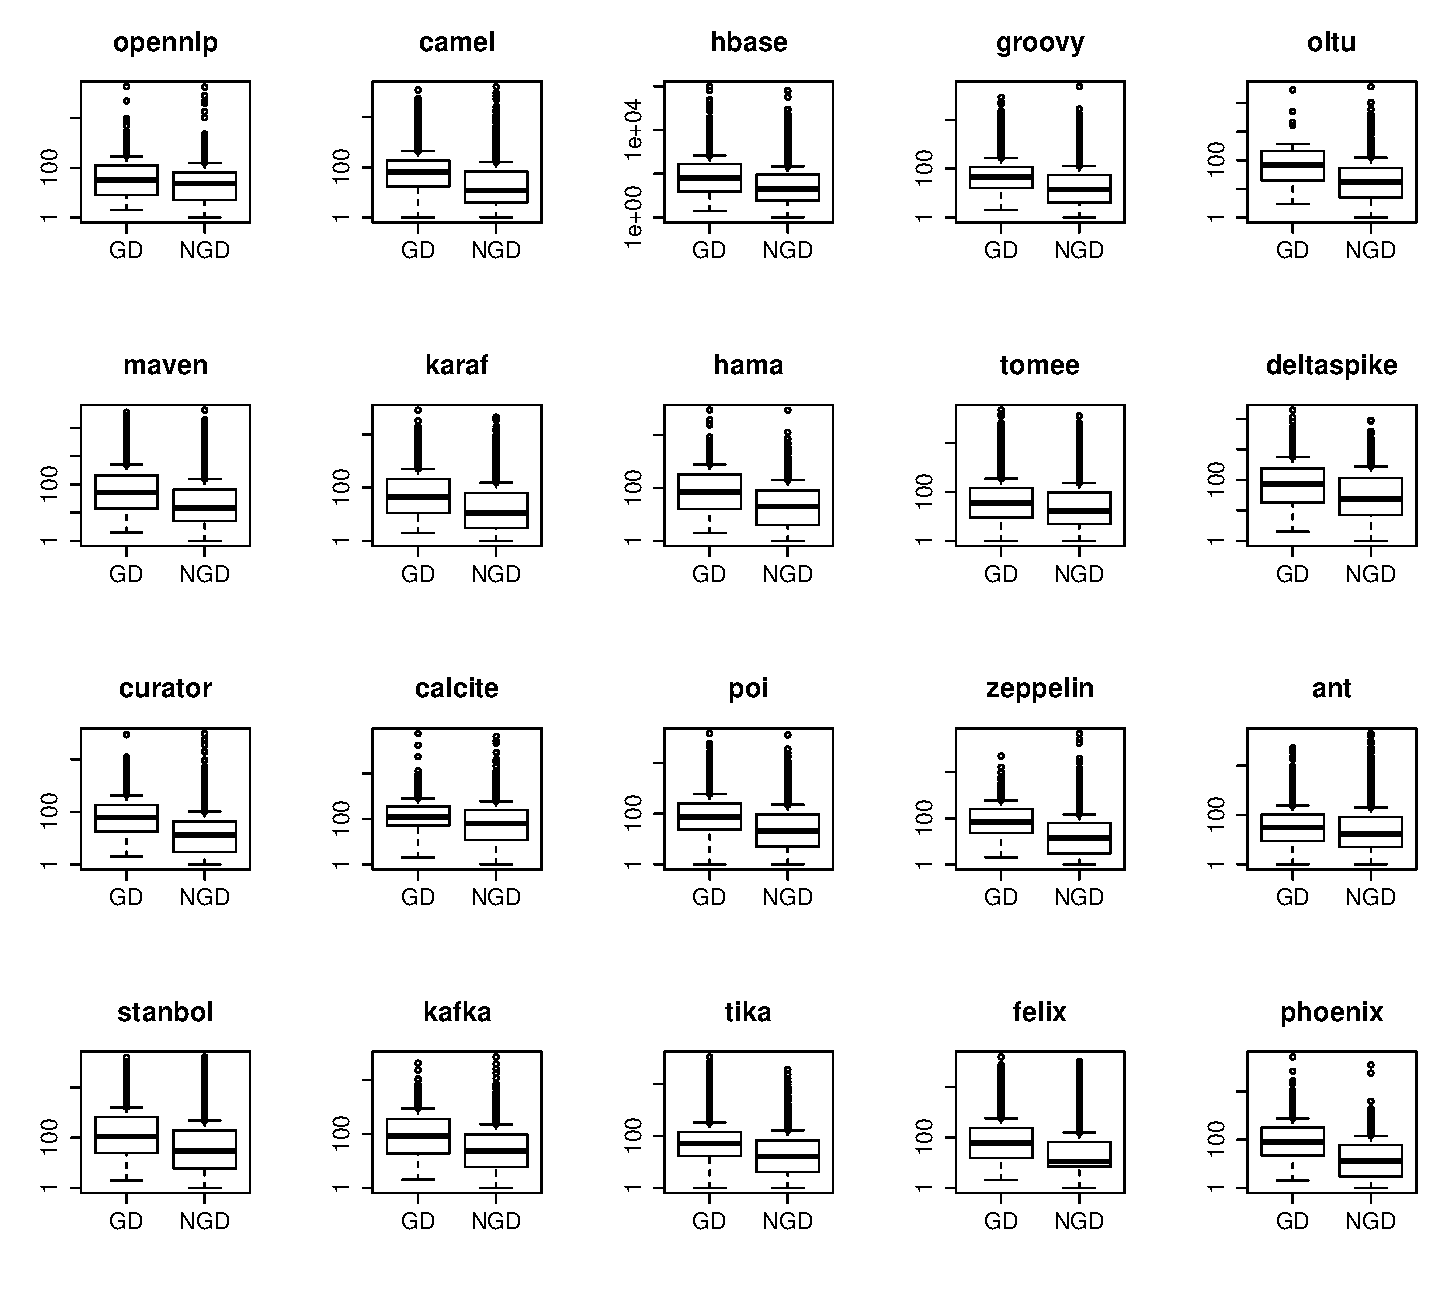
\includegraphics[width=100mm]{figures/chapter4/rq3_god_churn_logged_1}
	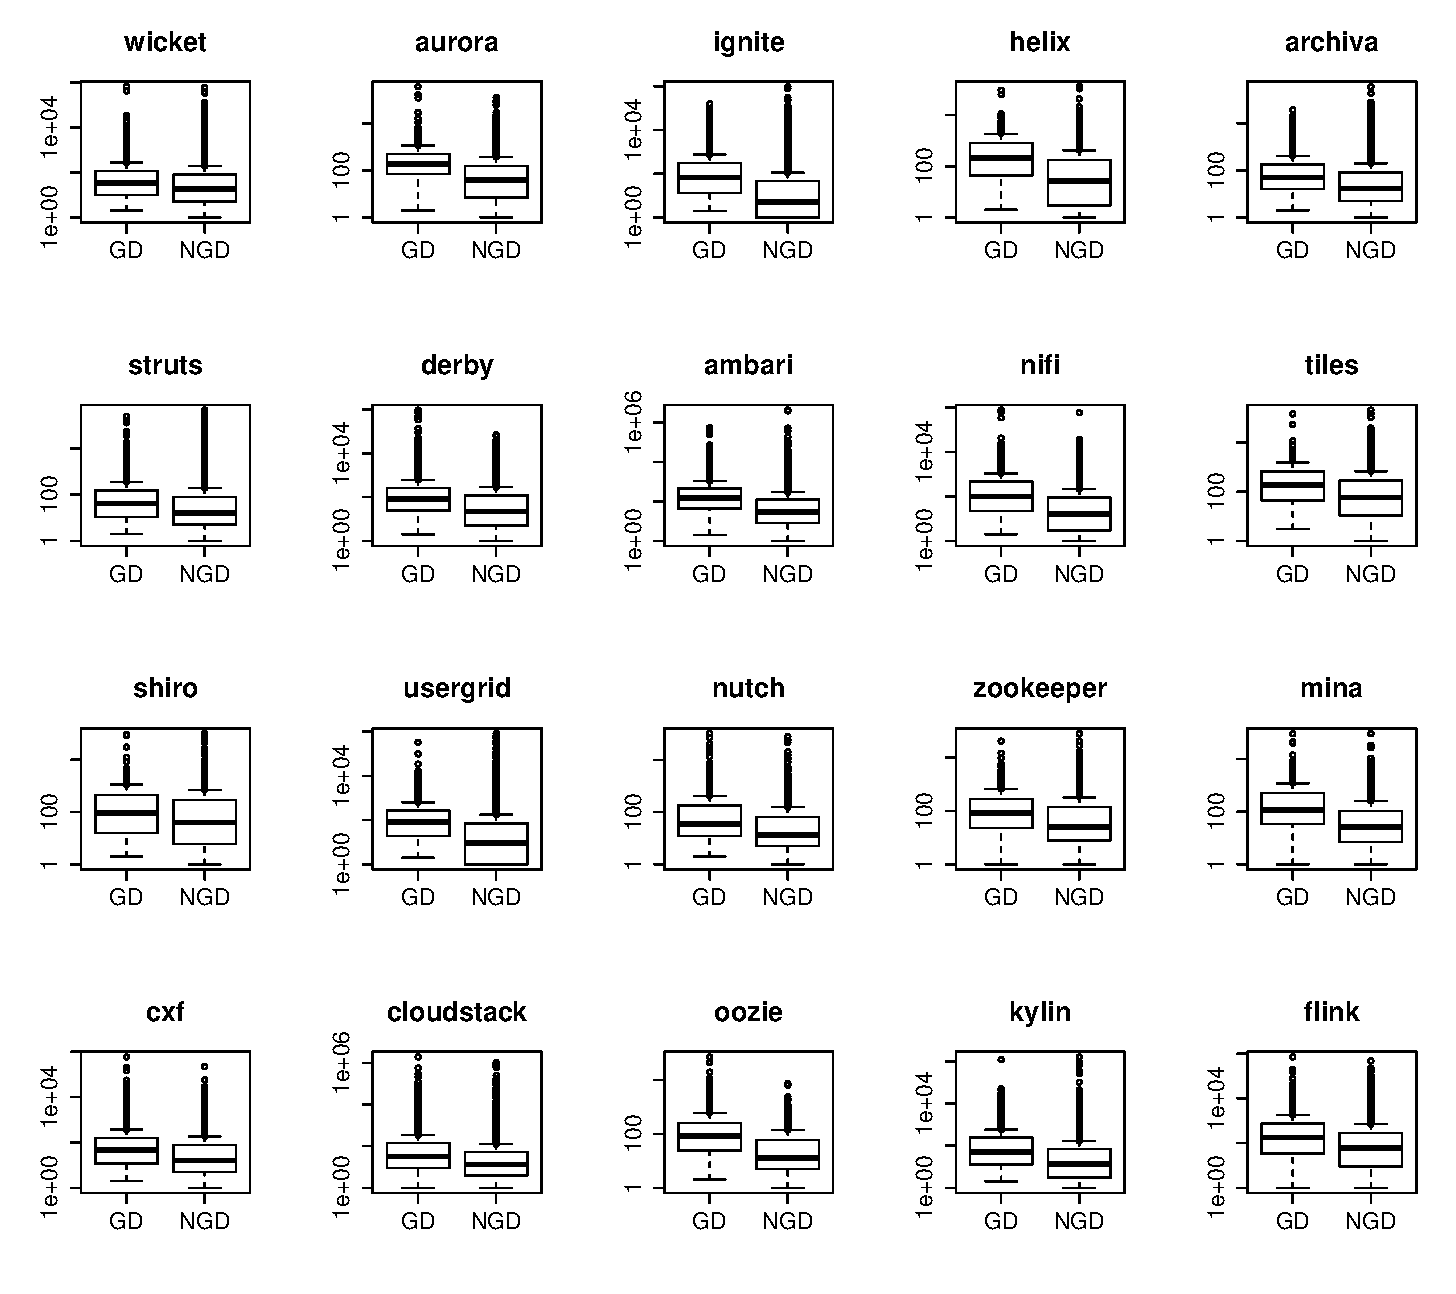
\includegraphics[width=100mm]{figures/chapter4/rq3_god_churn_logged_2}
	\caption{Total number of lines modified per change (GOD vs. NGOD).}
	\label{figure:total_number_of_lines_changed_god_vs_ngod}
\end{figure}


\begin{figure}[tb]
	\centering
	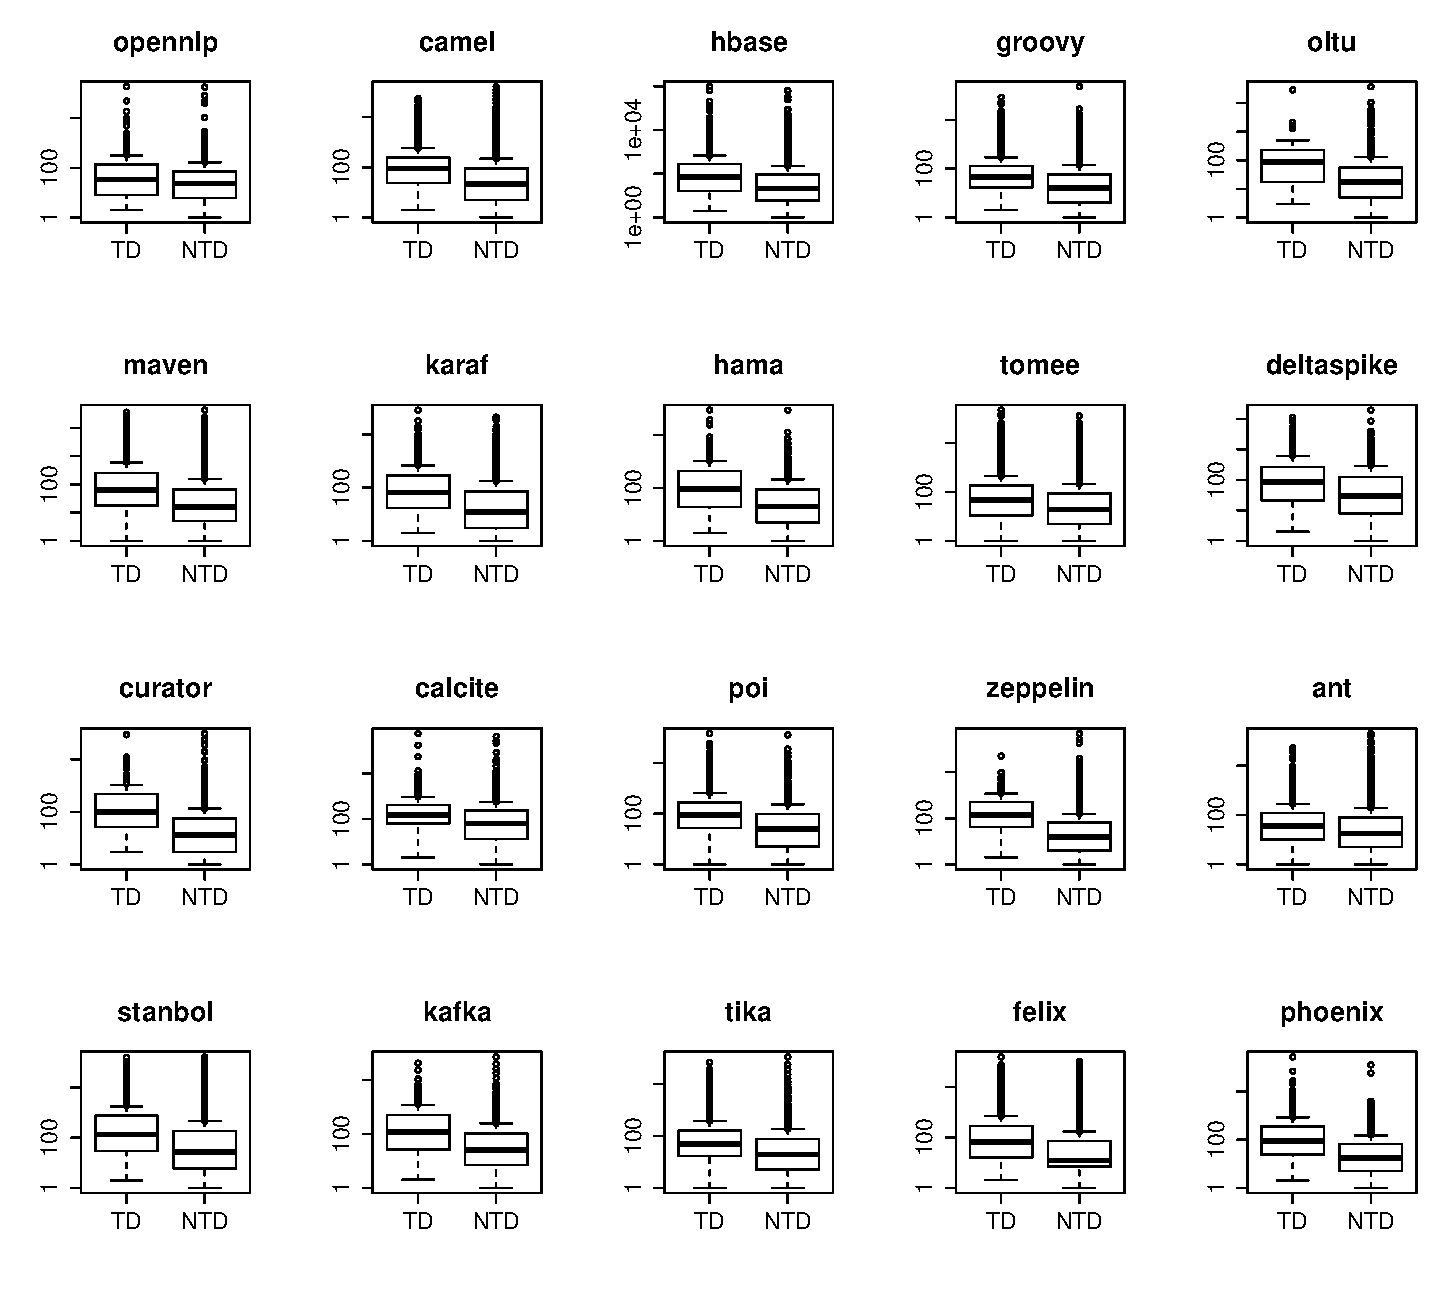
\includegraphics[width=100mm]{figures/chapter4/rq3_td_churn_logged_1}
	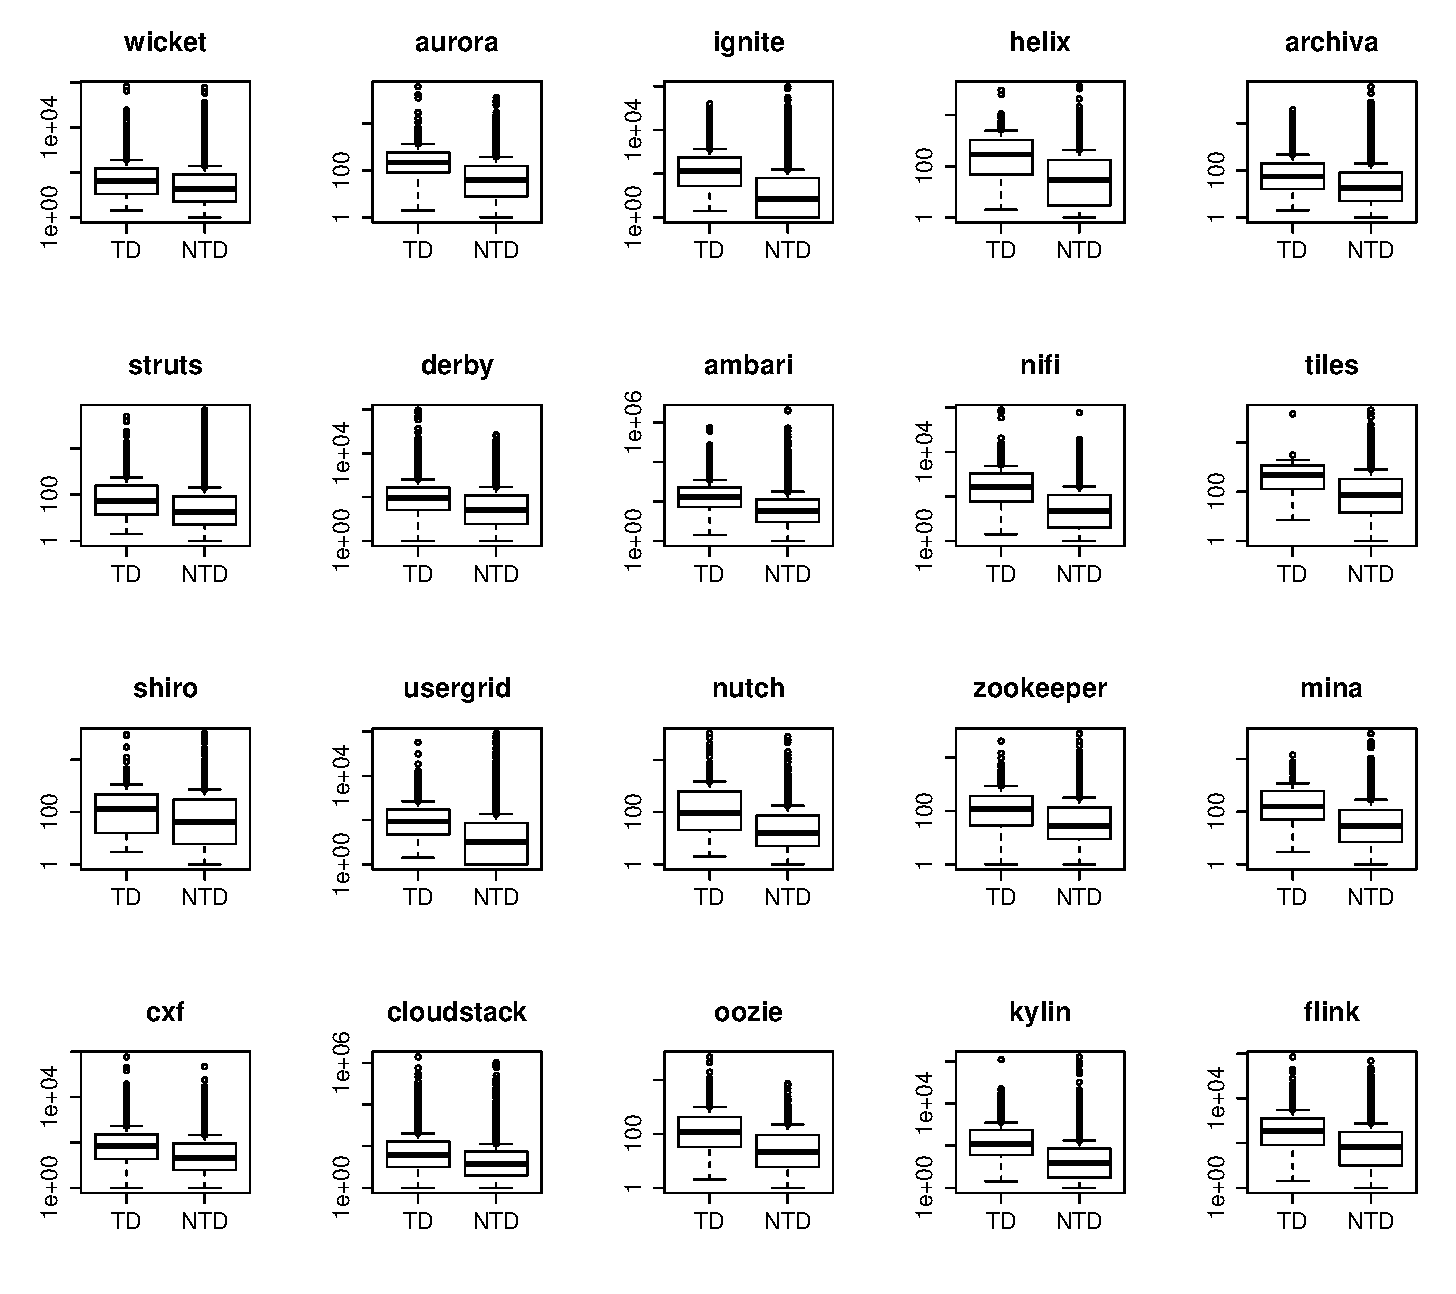
\includegraphics[width=100mm]{figures/chapter4/rq3_td_churn_logged_2}
	\caption{Total number of lines modified per change (TD vs. NTD).}
	\label{figure:total_number_of_lines_changed_td_vs_ntd}
\end{figure}


\begin{figure}[tb]
	\centering
	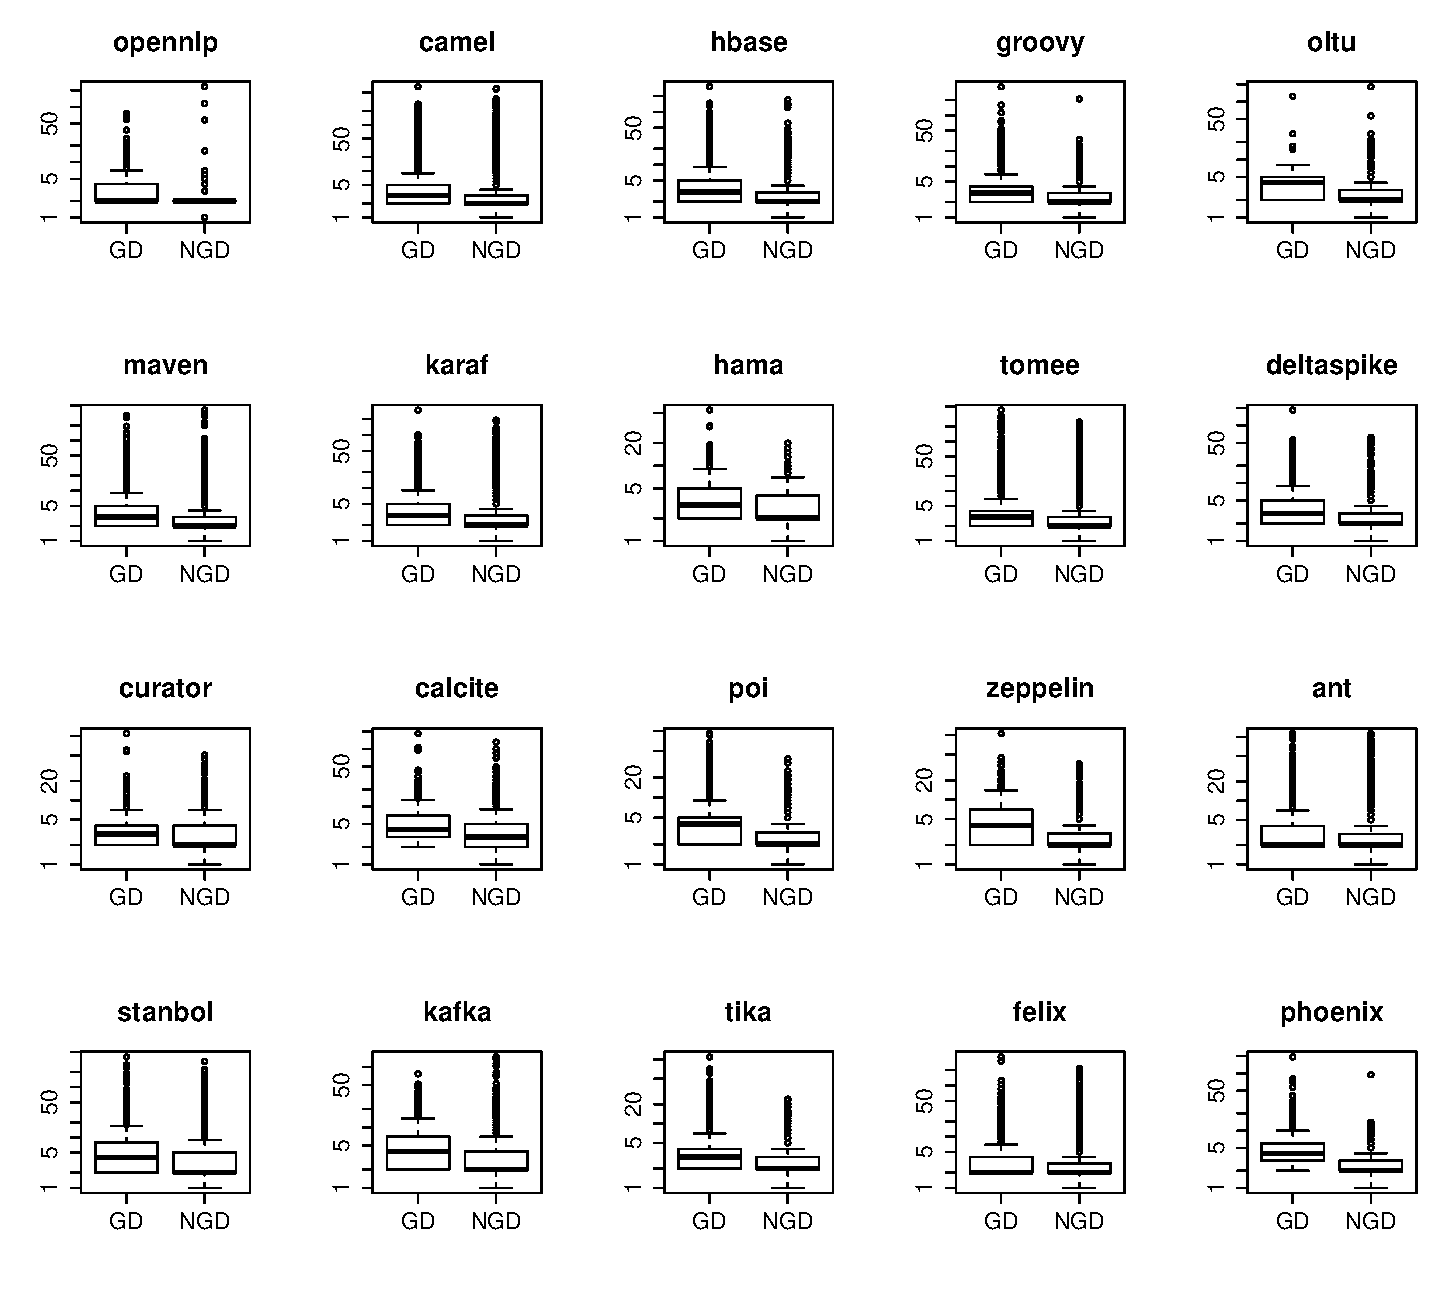
\includegraphics[width=100mm]{figures/chapter4/rq3_god_nd_logged_1}
	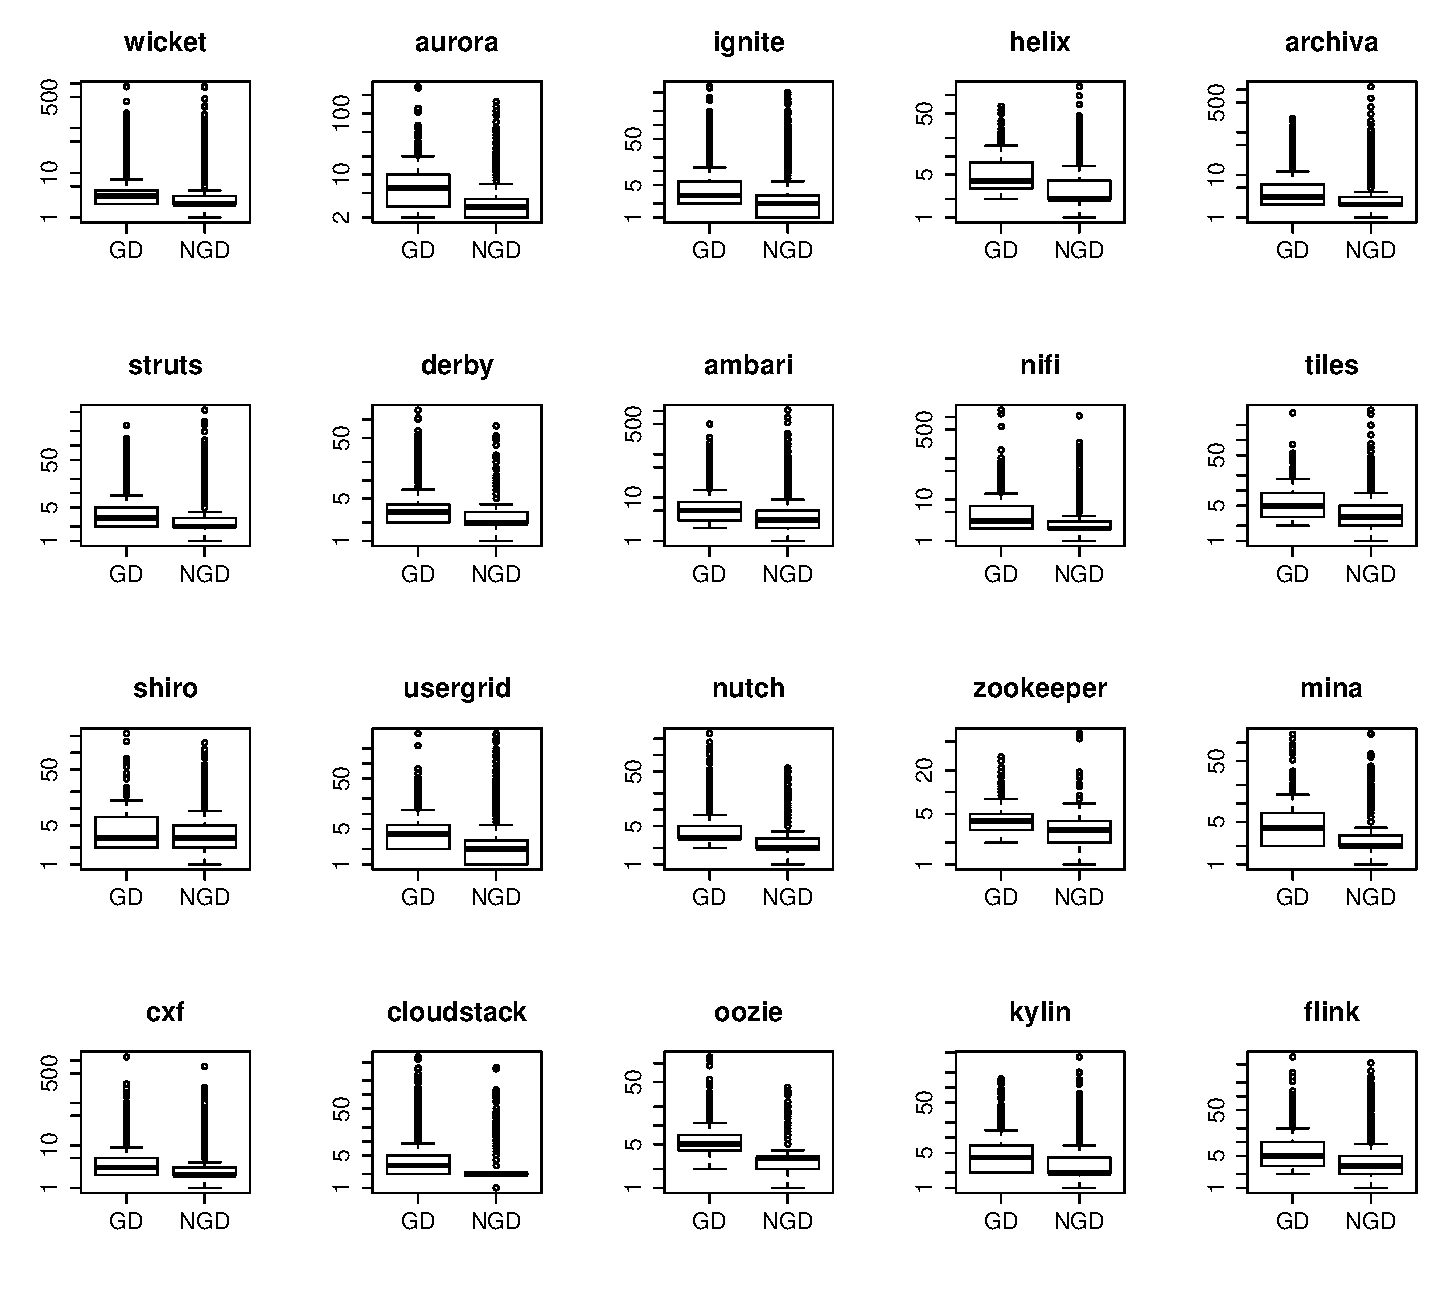
\includegraphics[width=100mm]{figures/chapter4/rq3_god_nd_logged_2}
	\caption{Total number of modified directories per GOD and NGOD change}
	\label{figure:total_nd_changed_god_vs_ngod}
\end{figure}


\begin{figure}[tb]
	\centering
	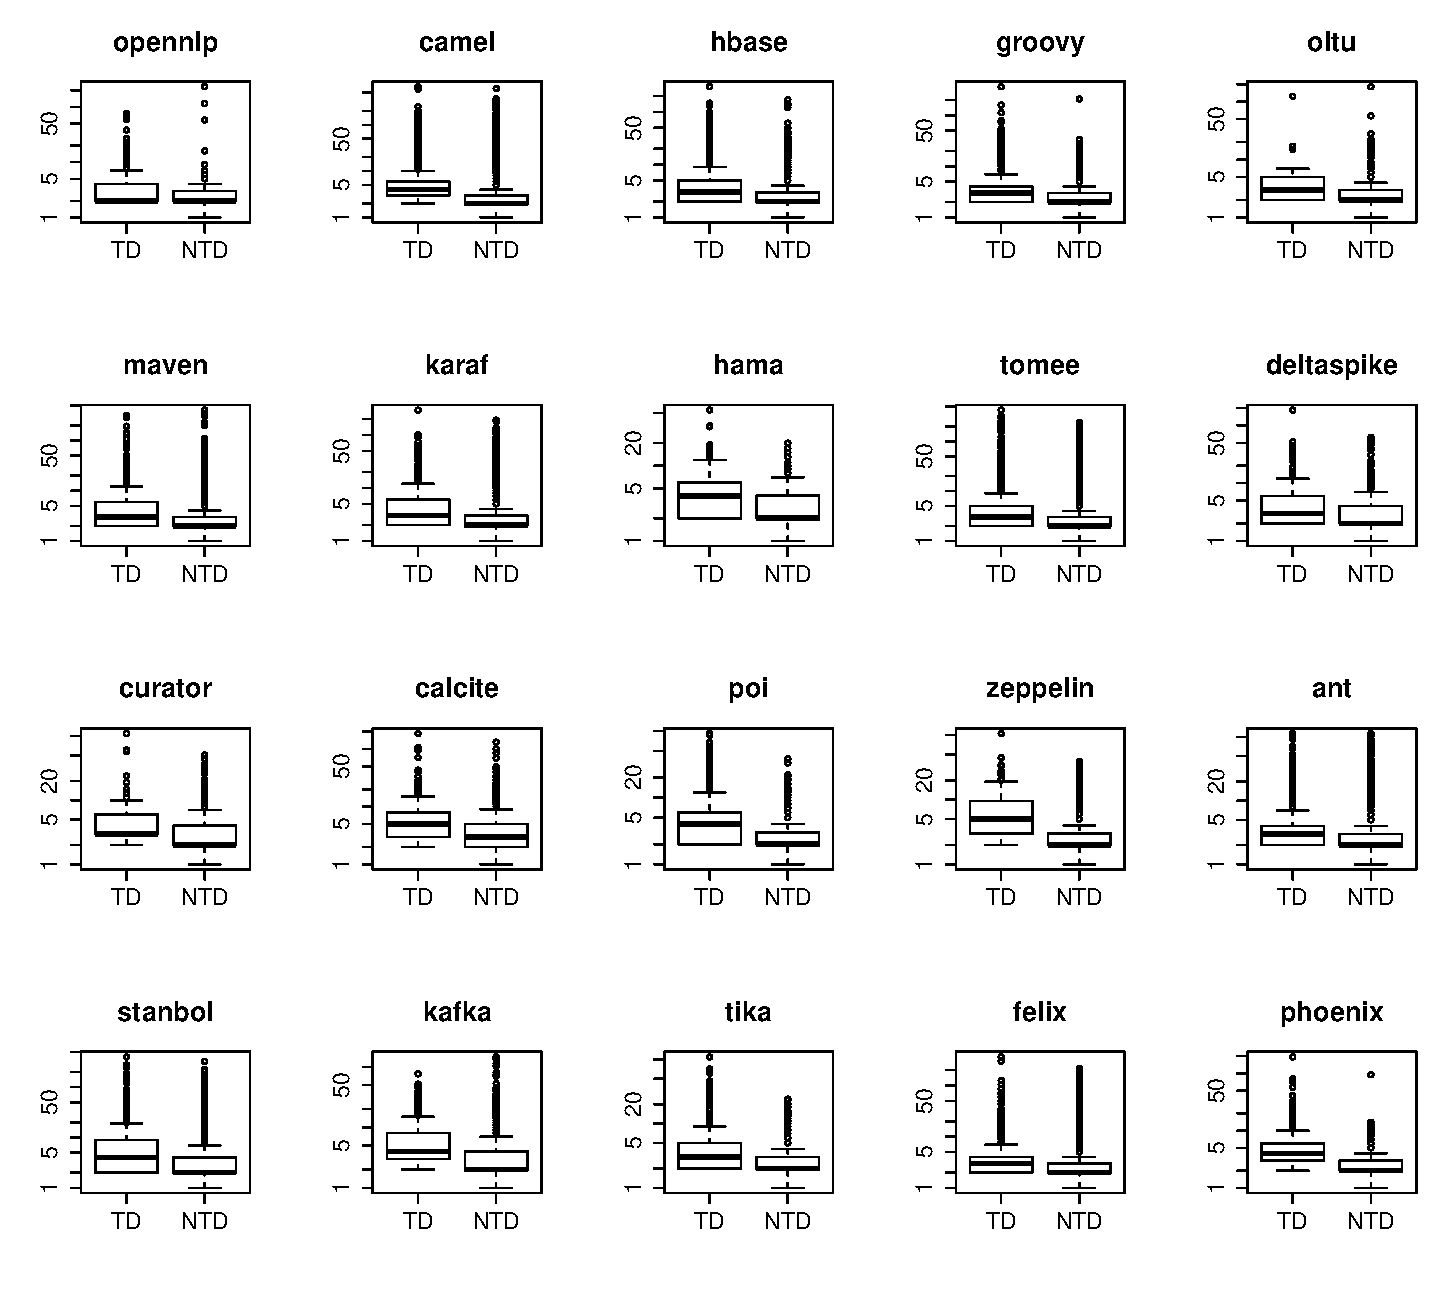
\includegraphics[width=100mm]{figures/chapter4/rq3_td_nd_logged_1}
	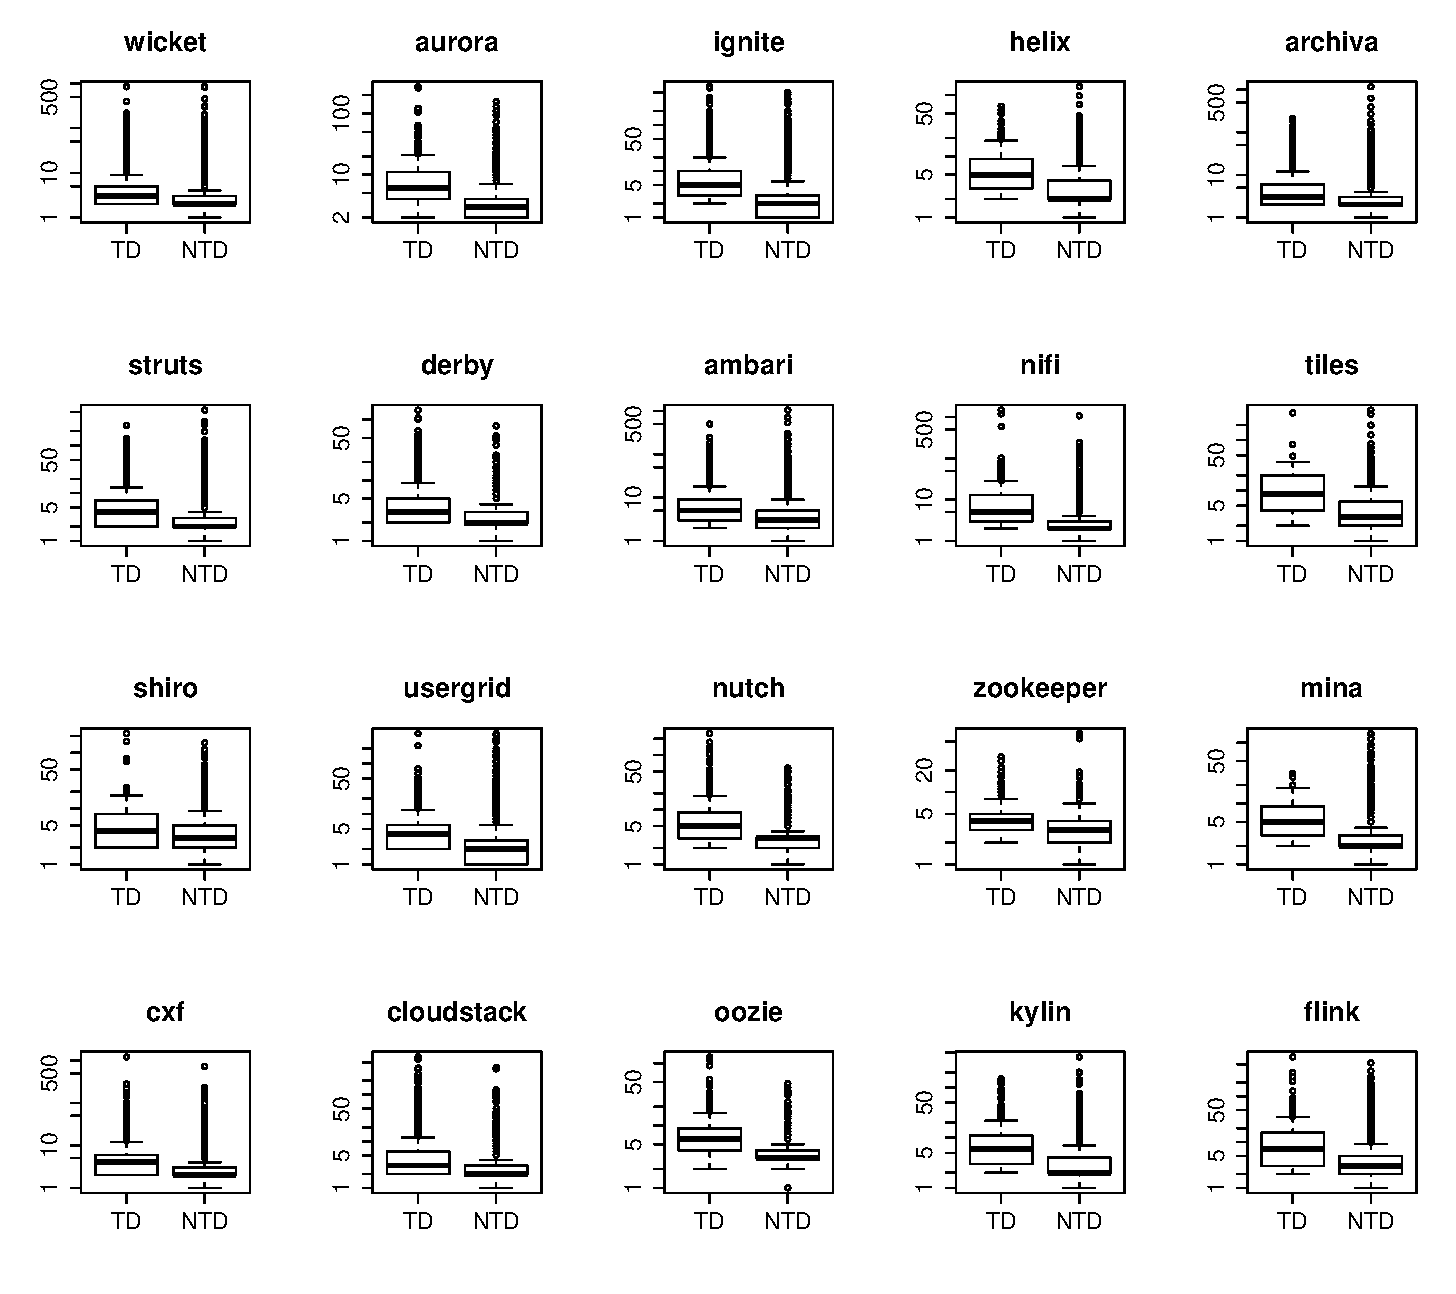
\includegraphics[width=100mm]{figures/chapter4/rq3_td_nd_logged_2}
	\caption{Total number of modified directories per SATD and NSATD change.}
	\label{figure:total_nd_changed_td_vs_ntd}
\end{figure}



\begin{figure}[tb]
	\centering
	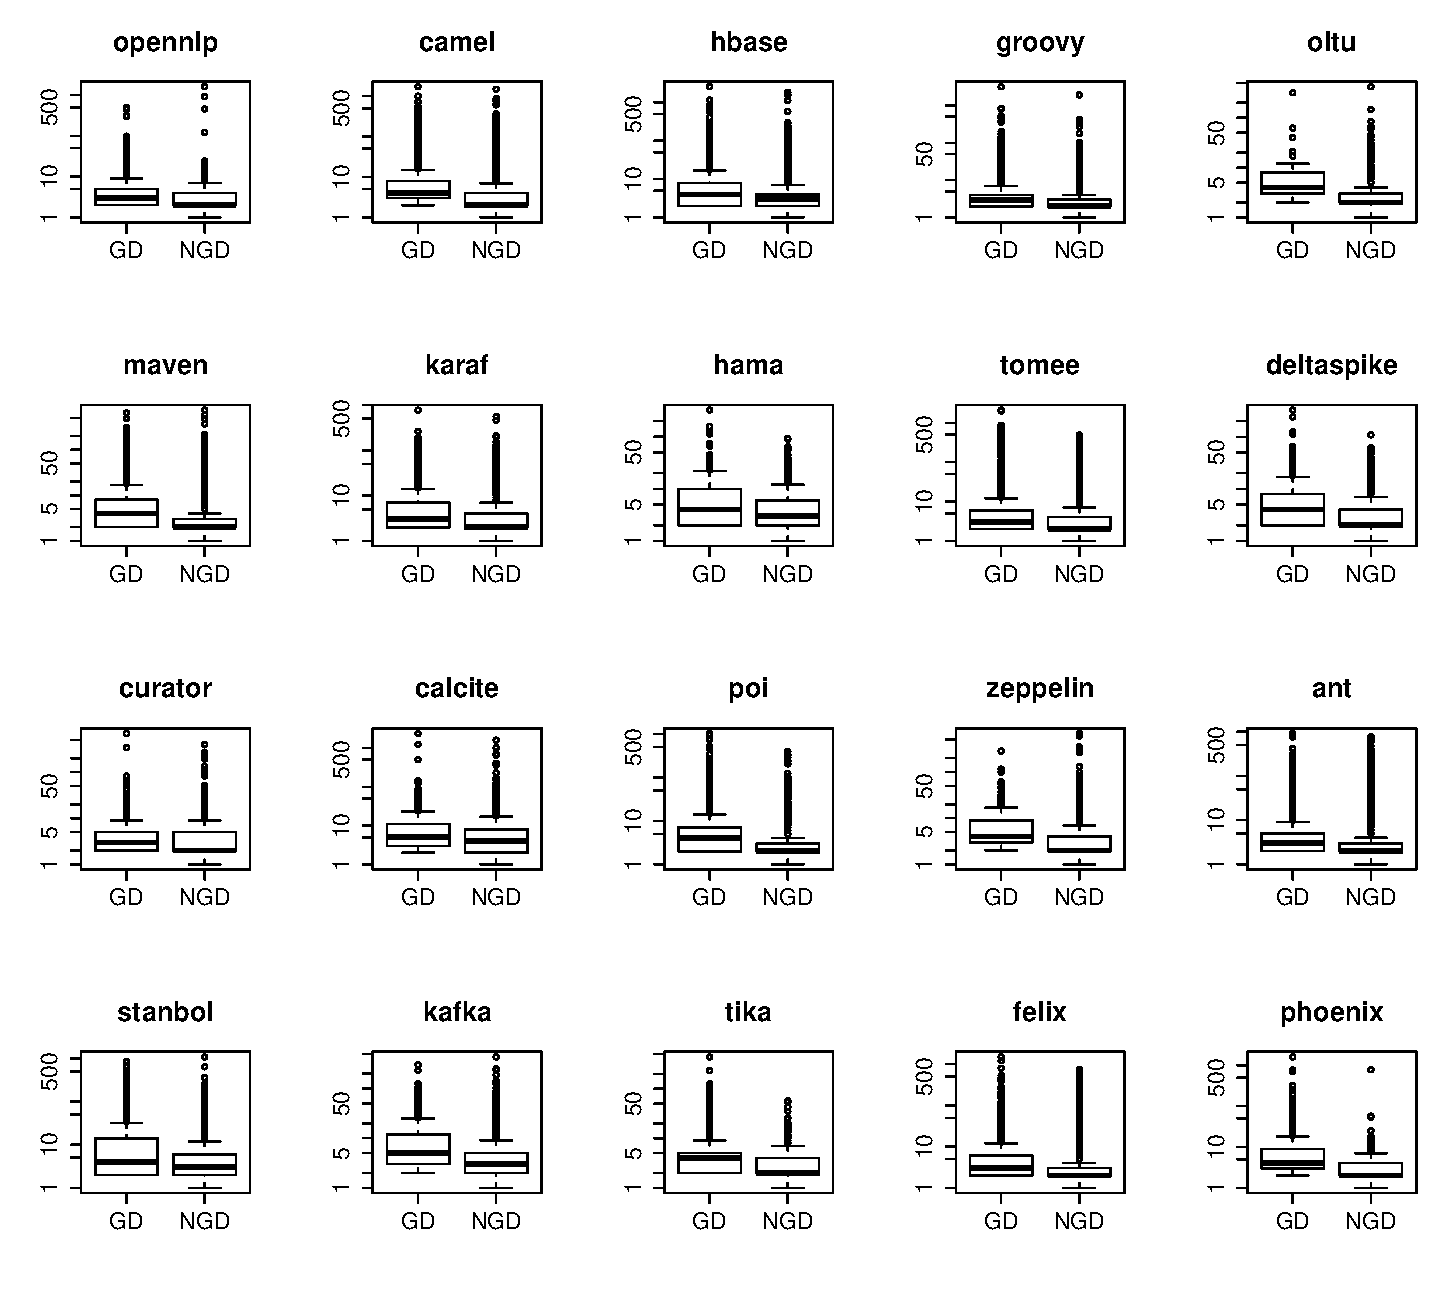
\includegraphics[width=100mm]{figures/chapter4/rq3_god_nf_logged_1}
	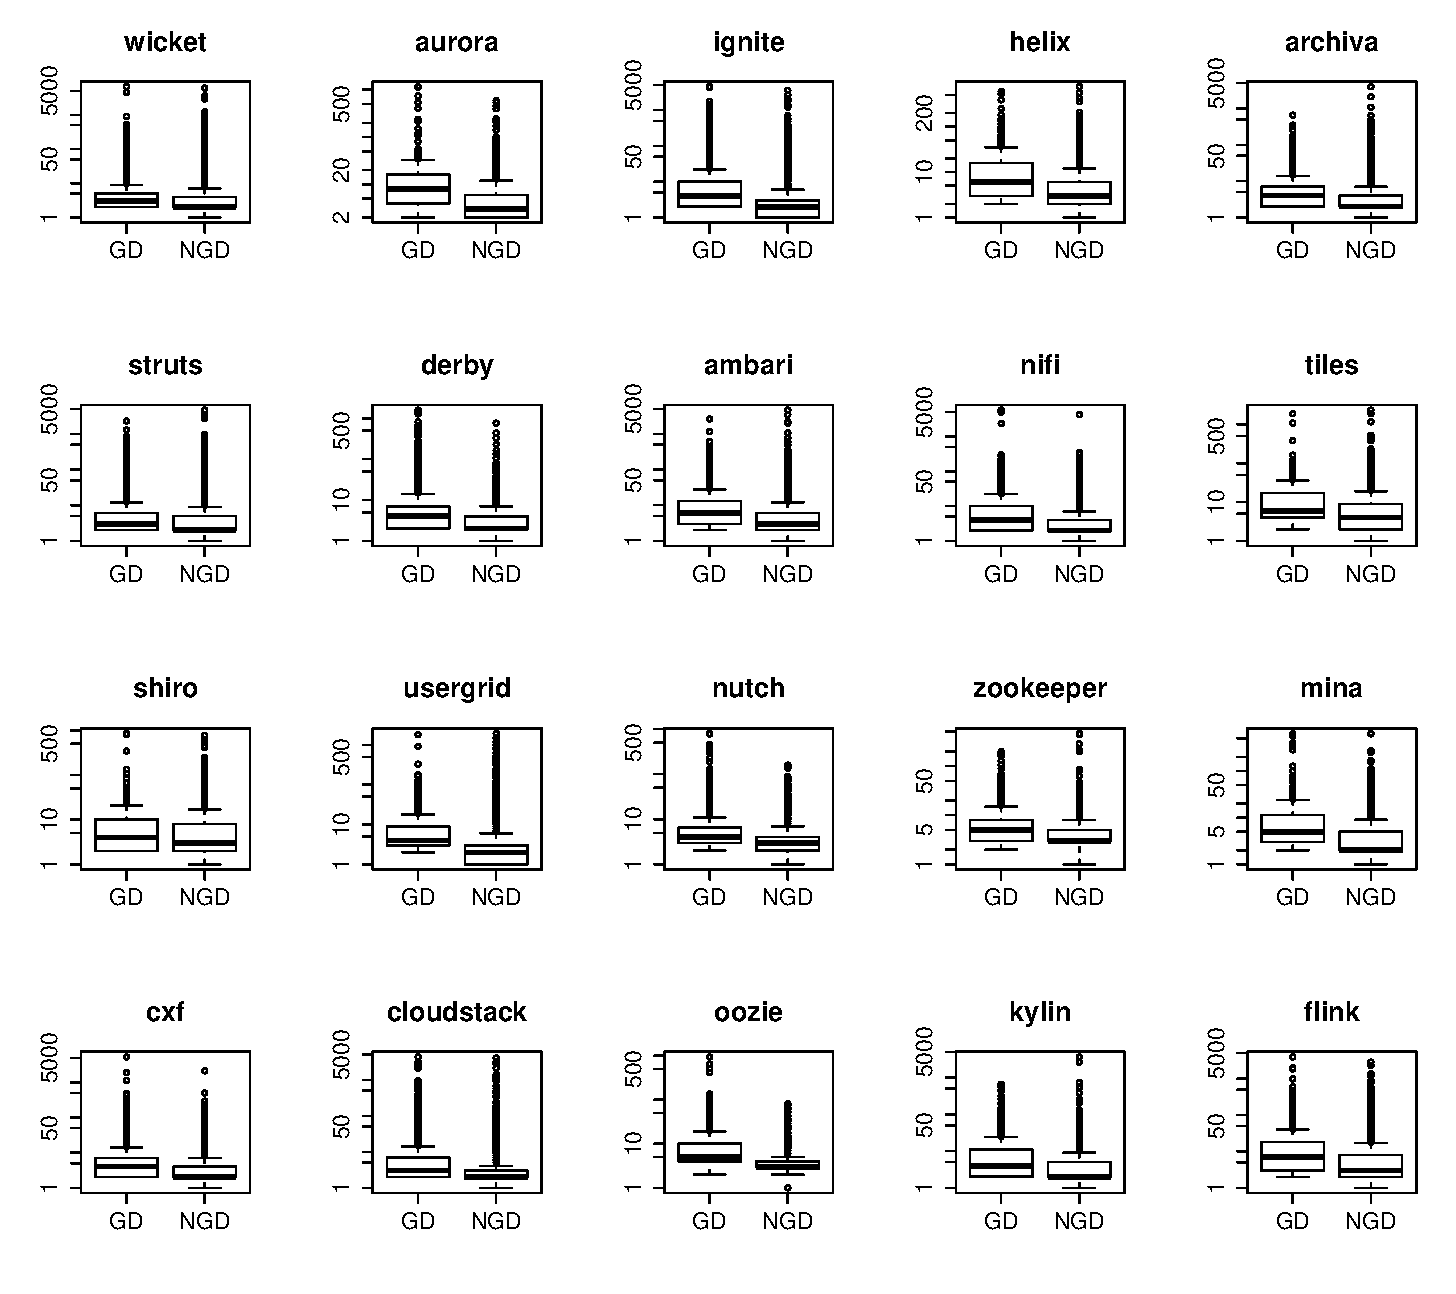
\includegraphics[width=100mm]{figures/chapter4/rq3_god_nf_logged_2}
	\caption{Total number of files modified per change (GOD vs. NGOD).}
	\label{figure:total_files_god_vs_ngod}
\end{figure}


\begin{figure}[tb]
	\centering
	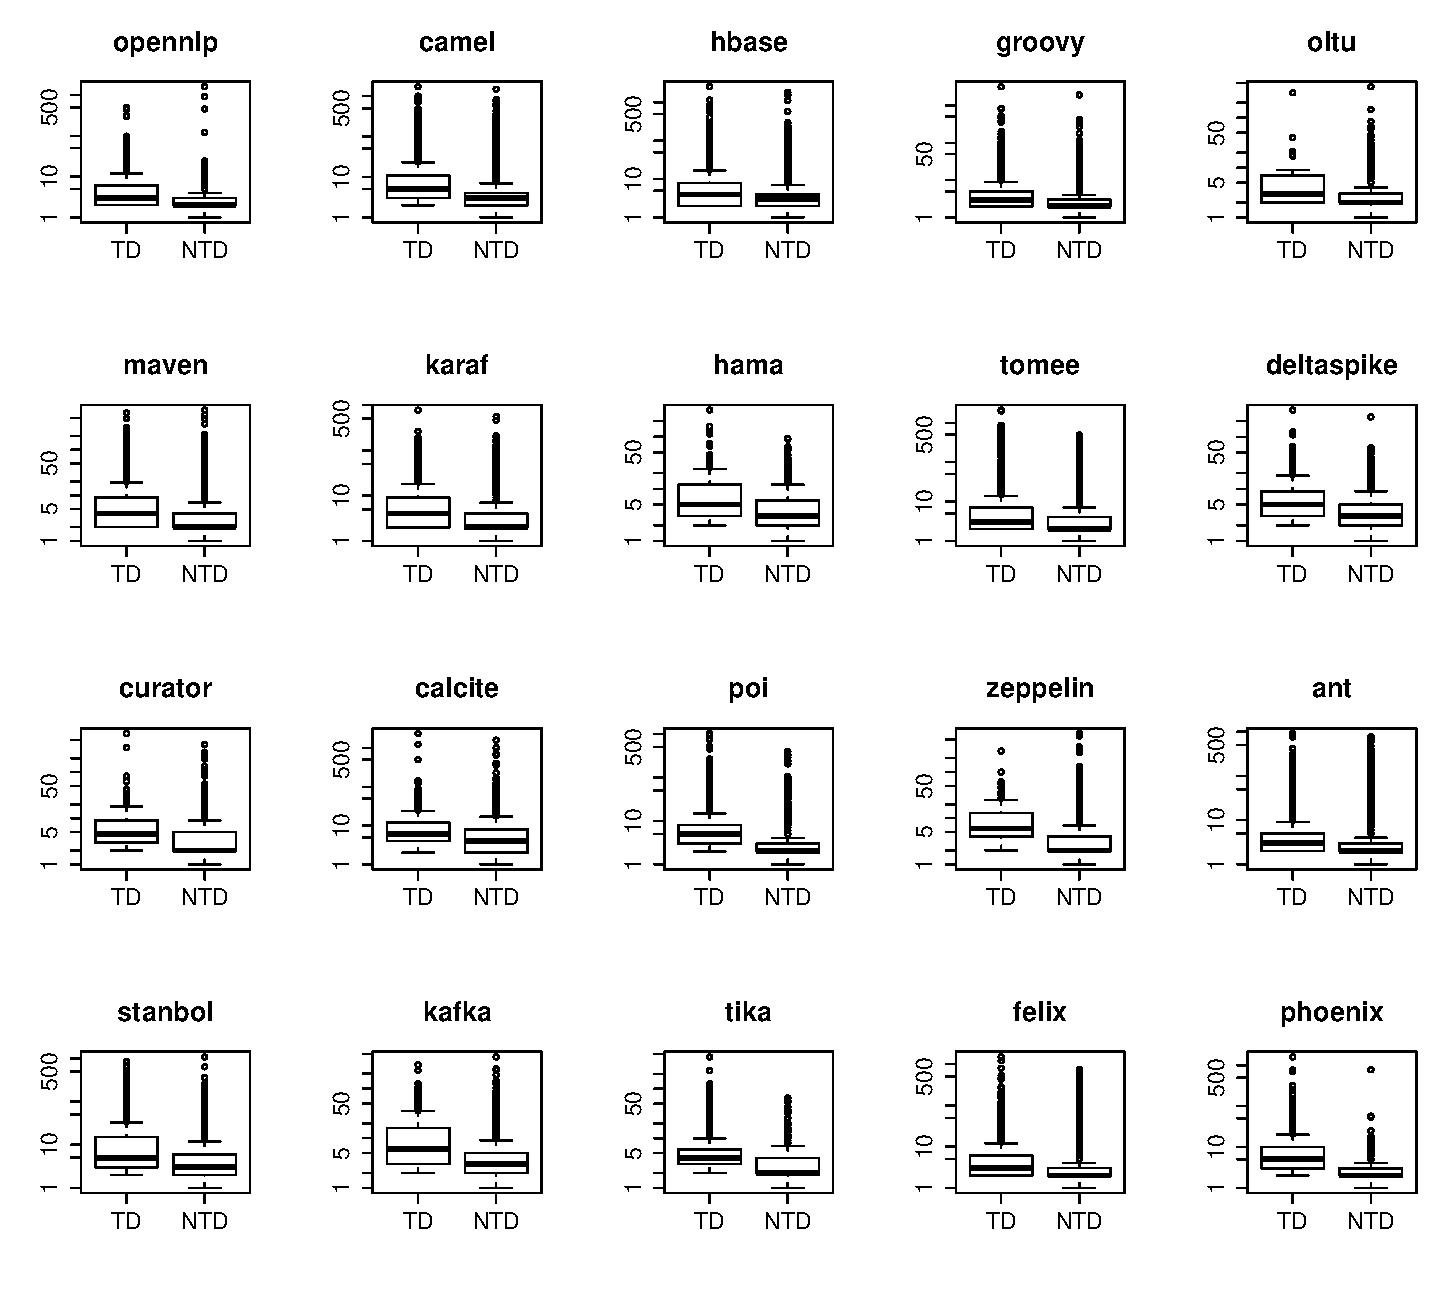
\includegraphics[width=100mm]{figures/chapter4/rq3_td_nf_logged_1}
	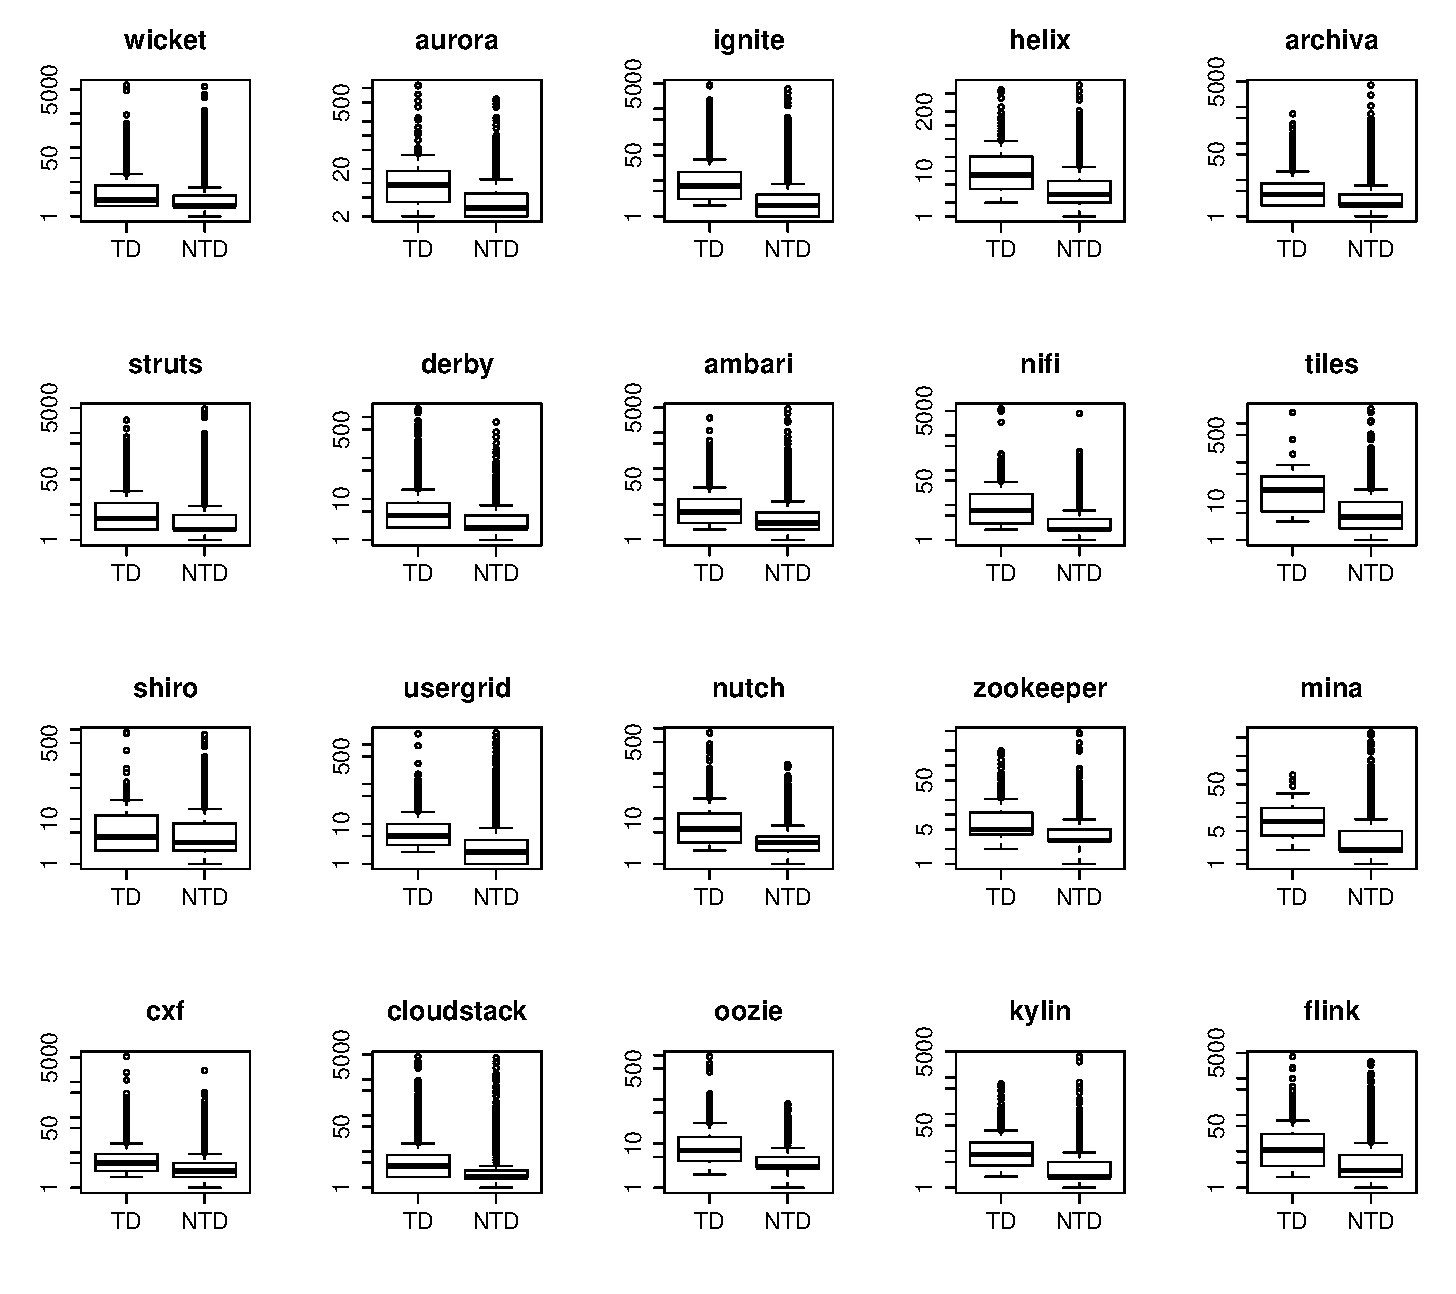
\includegraphics[width=100mm]{figures/chapter4/rq3_td_nf_logged_2}
	\caption{Total number of files modified per change (SATD vs. NSATD).}
	\label{figure:total_files_td_vs_ntd}
\end{figure}


\begin{figure}[tb]
	\centering
	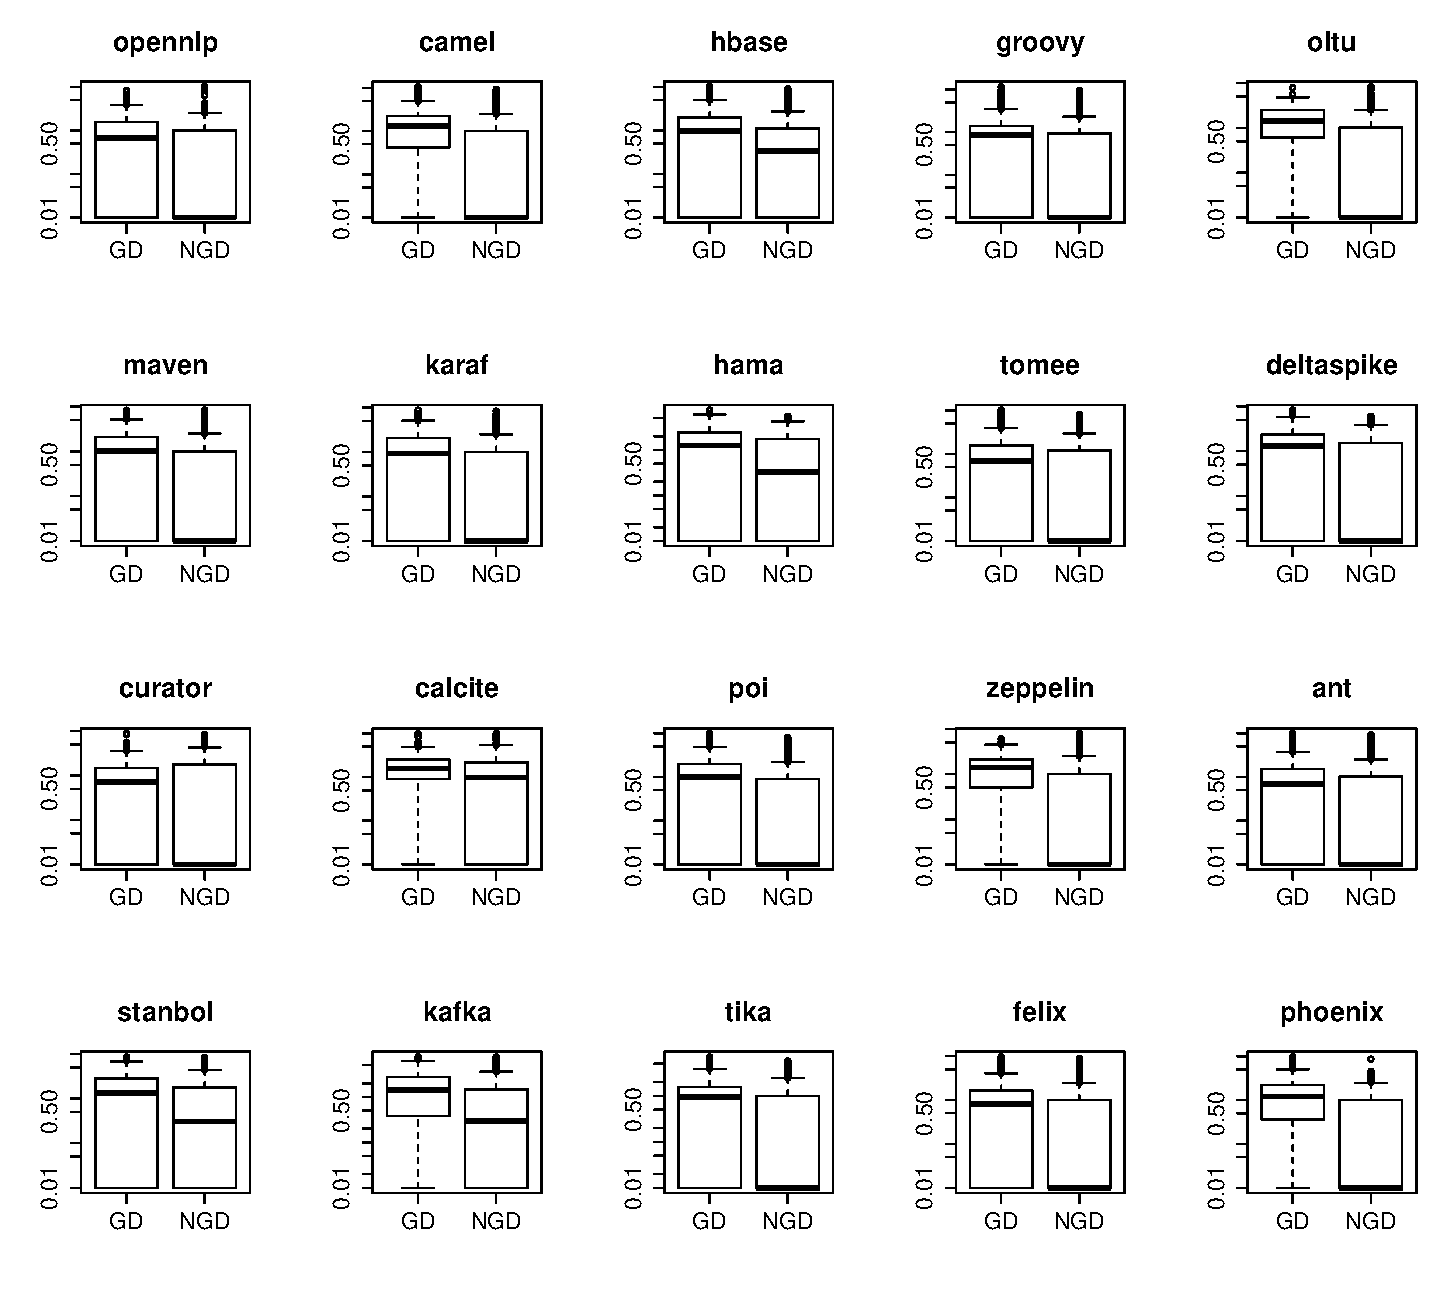
\includegraphics[width=100mm]{figures/chapter4/rq3_god_entropy_logged_1}
	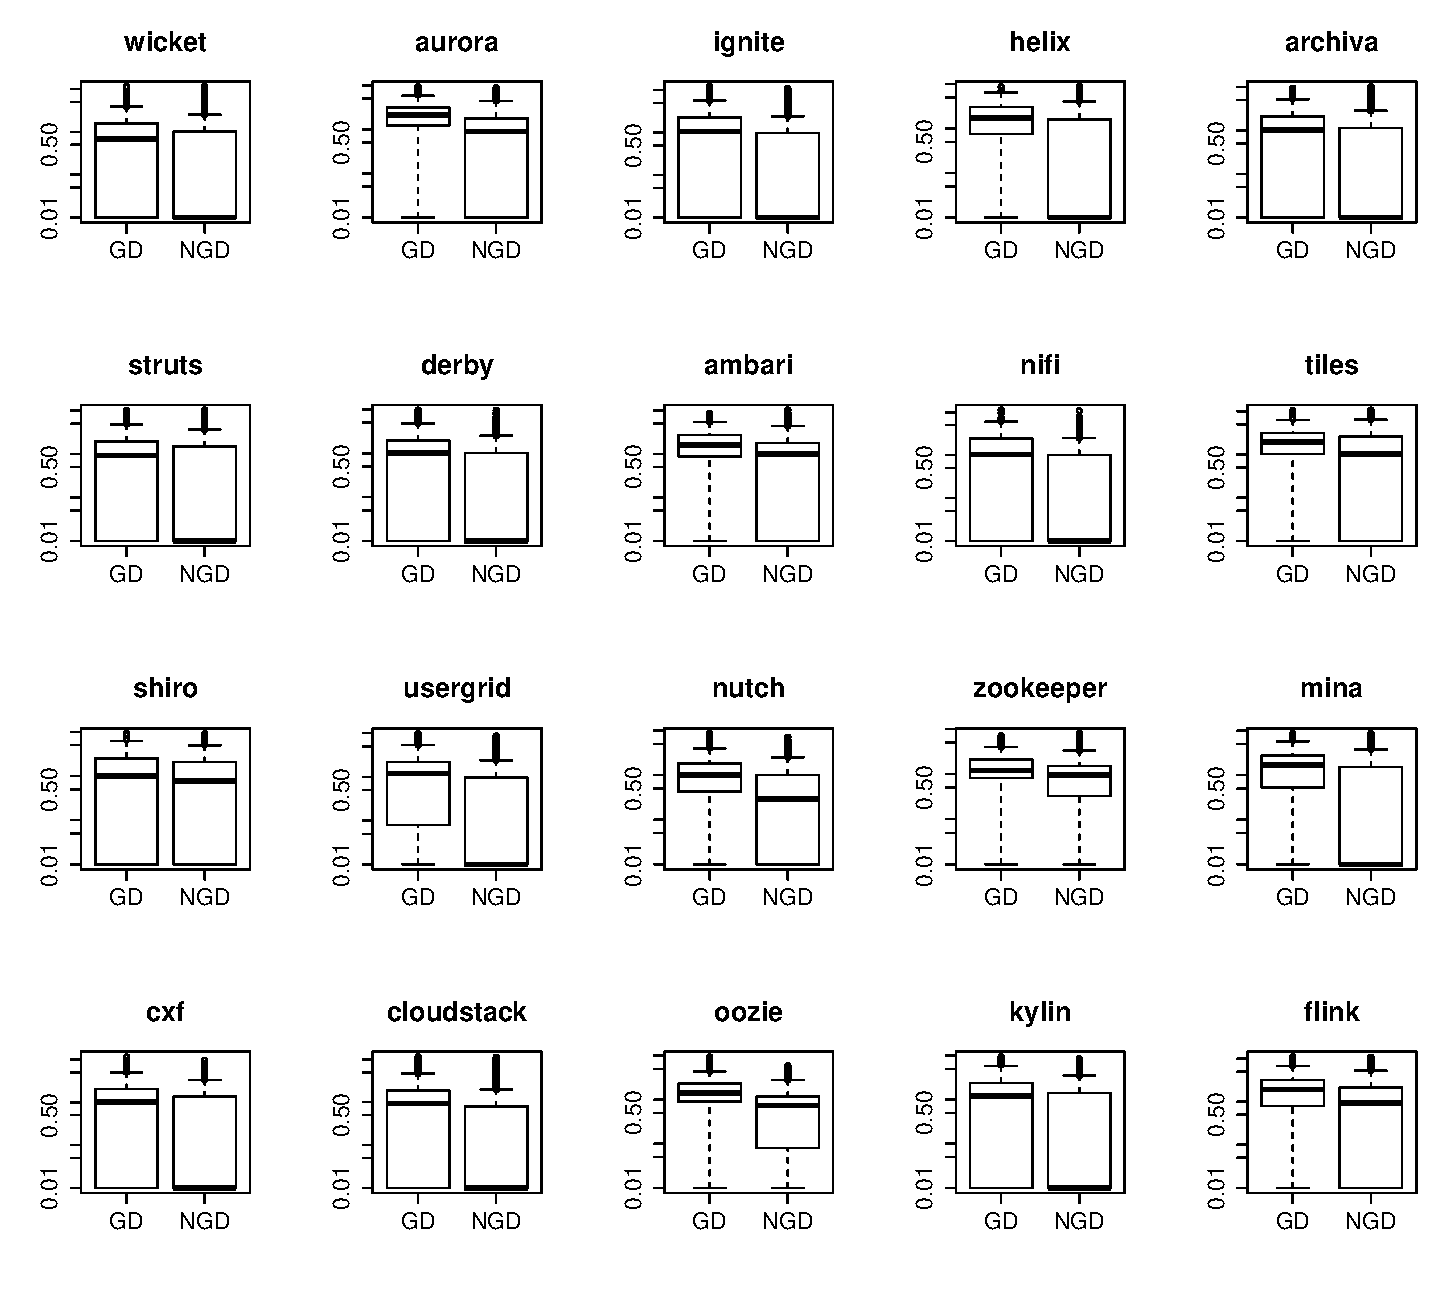
\includegraphics[width=100mm]{figures/chapter4/rq3_god_entropy_logged_2}
	\caption{Total number of entropy modified per change (GOD vs. NGOD).}
	\label{figure:total_entropy_god_vs_ngod}
\end{figure}


\begin{figure}[tb]
	\centering
	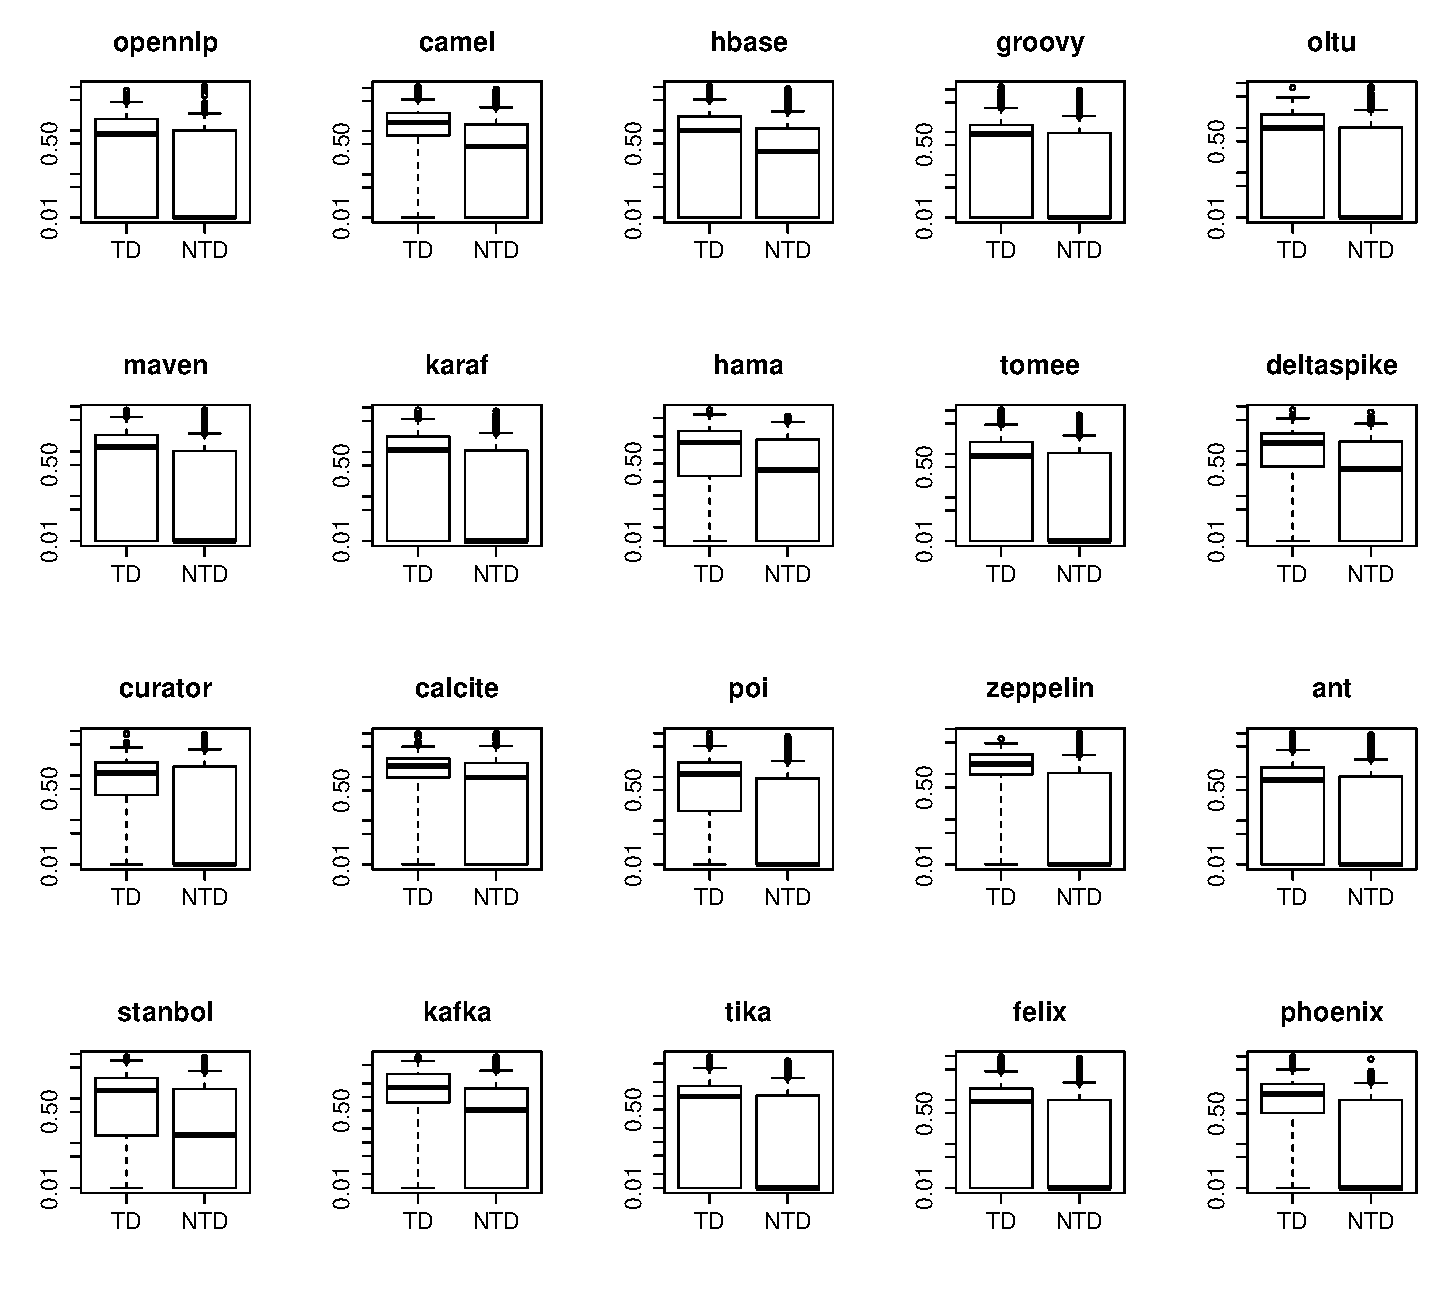
\includegraphics[width=100mm]{figures/chapter4/rq3_td_entropy_logged_1}
	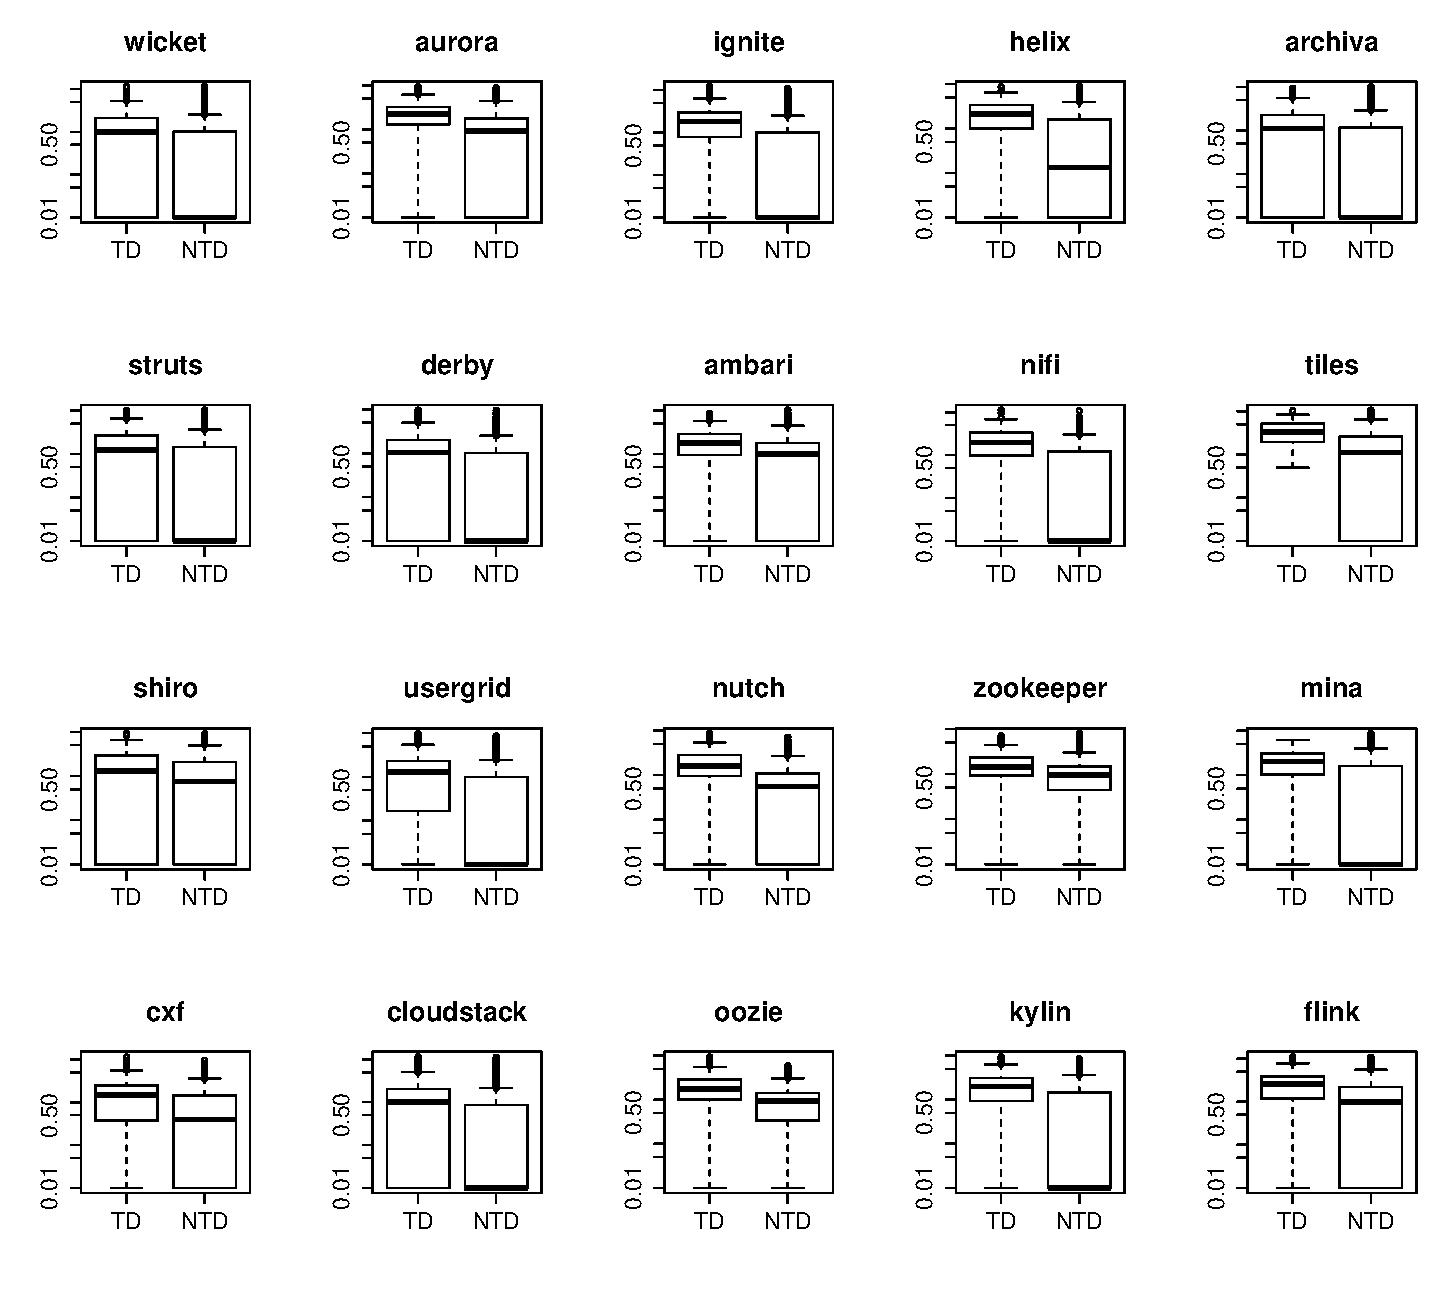
\includegraphics[width=100mm]{figures/chapter4/rq3_td_entropy_logged_2}
	\caption{Total number of entropy modified per change (SATD vs. NSATD).}
	\label{figure:total_entropy_td_vs_ntd}
\end{figure}



\end{appendices}

\addcontentsline{toc}{chapter}{Bibliography}
\bibliography{bibliography.bib}  
\bibliographystyle{abbrv}
\end{document}